No capítulo anterior, exploramos a análise de sentimento das postagens de eventos de zeladoria pública e a metodologia dos modelos de classificação baseado em aprendizagem de máquina; categorizamos os usuários em duas personas: \textit{helper} e \textit{complainers}. Personas com postagens predominantemente \textit{helper} são proativos, transmitindo mensagens construtivas e buscando colaborar para o bem-estar da comunidade incentivando uma coletividade. Em contraste, os \textit{complainers} são mais críticos, frequentemente apontando falhas e expressando insatisfações, muitas vezes motivados por questões individualistas. Além disso, capturamos o score de sentimento expresso nas postagens dos usuários em um modelo regressivo que varia de -1 para postagens com sentimento negativo e 1 para postagens com sentimento positivo. Neste capítulo, exploraremos como essas informações podem ser utilizadas para calcular a pressão social hiperlocal, com a intenção entender como as preocupações dos cidadãos se disseminam na rede e permitindo uma análise contextualizada dos discursos.

Cada postagem no Colab é mais do que uma simples expressão de sentimentos; ela está diretamente vinculada a eventos específicos de zeladoria pública, com tipos de eventos pré-definidos, que dão contexto ao conteúdo compartilhado. Estes tipos de evento de zeladoria podem variar desde preocupações com segurança, como 'Ponto de tráfico de drogas', até perturbações como 'Ponto recorrente de Poluição Sonora' ou questões ambientais como 'Poda de Árvore'. A combinação desses tipos de eventos, o score de sentimento das postagens e as personas classificadas e a localização do evento, oferece uma visão holística das interações dos cidadãos na plataforma, permitindo uma compreensão mais aprofundada das preocupações e necessidades da comunidade. Nesse sentido, podemos considerar o Colab como uma ferramenta inovadora para monitoramento e análise de sentimentos em tempo real, capturando a essência das preocupações e sentimentos dos cidadãos em reação a mudanças que ocorrem no ambiente urbano. Ao categorizar postagens por eventos específicos, a plataforma fornece insights valiosos para tomadores de decisão, pesquisadores e outros stakeholders.

Portanto, consideramos que o Colab além de ser um aplicativo móvel, uma rede social de cidadania e uma empresa de GovTech, pode ser entendido também como o que viemos a chamar de 'Barômetro Social Hiperlocal'. Este conceito sugere que a plataforma não apenas capta as opiniões e sentimentos dos cidadãos, mas o faz levando em consideração as particularidades de diferentes localidades e temáticas. Assim, cada feedback fornecido pelos usuários pode ser interpretado como uma medida da 'pressão' social de uma área ou tema específico. O termo 'barômetro social' geralmente se refere à capacidade de medir a opinião pública. No entanto, ao adicionar 'hiperlocal', estamos destacando a especificidade geográfica e temática das opiniões. O Colab exemplifica esse conceito, permitindo uma análise contextualizada dos discursos tanto em diferentes localidades quanto em variados assuntos. Autoridades, organizações e cidadãos podem se beneficiar dessa ferramenta, obtendo uma compreensão mais profunda das preocupações locais e adaptando suas ações e políticas de acordo. Aplicativos como o Colab não apenas fornecem uma plataforma para participação cidadã, mas também se estabelecem como um instrumento vital para a tomada de decisões informadas em uma sociedade cada vez mais conectada e dinâmica. Os usuários do Colab não apenas expressam seus sentimentos e opiniões sobre eventos de zeladoria pública, mas também o fazem de forma geolocalizada e categorizada por tipo de evento. Esta característica única da plataforma a diferencia de outras redes sociais, como o Twitter, onde a opinião média sobre um tópico específico pode ser mais difícil de discernir devido à falta de categorização e geolocalização.

Durante a classificação manual das postagens para análise de sentimento e personas conduzida no capítulo anterior, identificamos padrões relacionados a tipos de eventos e sentimentos dos usuários. Por exemplo, postagens relacionadas à gentrificação mostram preocupações com a valorização imobiliária. Alguns usuários tendem a criar eventos de zeladoria no Colab destacando uma preocupação com a valorização ou desvalorização dos seus imóveis. Outras postagens refletem tensões sobre a presença de pessoas em situação de rua, enquanto algumas destacam preocupações com poluição sonora ou gestão da vegetação urbana. Além disso, postagens sobre gestão de resíduos e qualidade do ar indicam uma crescente conscientização ambiental. Alguns usuários também tendem a incorporar discursos políticos ou fiscais reverberando debates sobre governança e prestação de contas que acontecem fora das redes. Essa diversidade de tópicos revela a riqueza de insights que o Colab oferece sobre a dinâmica social e as prioridades locais. Nossa análise revelou que as preocupações dos cidadãos são variadas e contextualmente dependentes. O Colab reflete e amplifica as vozes dos cidadãos em questões locais. A geolocalização das postagens é fundamental para entender as preocupações específicas de cada comunidade, reforçando o caráter único do Colab como um barômetro social hiperlocal.

A singularidade do Colab está concentrada, principalmente, na produção e consumo de conteúdo em eventos de zeladoria pública. Estas postagens, categorizadas por tipos específicos de eventos e enriquecidas com informações geolocalizadas, fotos, comentários e \textit{likes} já fornecem aos stakeholders, especialmente às agências governamentais, uma perspectiva clara das necessidades e preocupações das comunidades. No entanto, ao adicionar uma camada de análise de sentimento, essa perspectiva pode se tornar ainda mais valiosa. Por exemplo, em um cenário em que uma mudança significativa é implementada, como a troca de empresas de coleta de lixo em uma cidade. A partir da análise dos dados produzido pelas interações do Colab, os tomadores de decisão podem monitorar em tempo real se a polaridade das postagens relacionadas a coleta de lixo piorou ou melhorou após essa mudança, servindo como um indicador da eficácia da decisão, ou, pelo menos, um indicador reação dos munícipes após essa mudança.

Assim, nossa hipotese é que aplicativos como o Colab não são apenas plataformas de interação, mas também podem ser entendidos como 'Barômetros Sociais Hiperlocais'. Esta perspectiva pode refinar os dados brutos da rede em um instrumento de \textit{feedback-loop}, não apenas para a expressão cidadã, eficácia de determinadas políticas públicas de acordo com o sentimento dos usuários. Ao compreender e responder às demandas expressas no Colab, as agências governamentais têm a oportunidade de aprimorar suas ações e políticas, garantindo uma gestão mais alinhada às necessidades e sentimentos das comunidades urbanas.

Entender o Colab como um 'Barômetro Social Hiperlocal' é informada e inspirada pelo conceito de Homogeneidade de Opiniões, conforme descrito por \citeonline{2023_Atiqi_BOOK}. A ideia de medir a pressão social de determinados assuntos ou temas nas comunidades da rede surgiu a partir da busca pela quantificação da homogeneidade de opiniões dos usuários.

\begin{citacao}
	'A more general concept defines echo chamber as the lack of information diversity a person is exposed with. The opinion does not necessarily have to be agreed by the person, but the type of opinions surrounding them should be homogeneous. A non-political example as suggested by Pentland is in the case of online trading (...) The lack of opinion diversity in this case is also considered as an echo chamber'. \cite[p. 17]{2023_Atiqi_BOOK}.
\end{citacao}

A homogeneidade de opiniões, conforme definido pelo autor, é um indicador-chave de câmaras de eco. Ao analisar padrões nas postagens e nos sentimentos expressos pelos usuários, é possível discernir se uma opinião ou perspectiva está sendo predominantemente reforçada. Também é possível entender a distribuição de opiniões entre os relacionamentos dos usuários na rede, verificando se a opinião é compartilhada por um grupo de amigos ou se é amplamente aceita por toda a rede. Essas heurísticas são cruciais para identificar câmaras de eco e podem ser aplicadas para detectar e mitigar a polarização de opiniões.

Câmaras de eco têm o potencial de distorcer a percepção da realidade e intensificar a polarização de opiniões, o que pode influenciar decisões políticas e a percepção das necessidades da comunidade. O Colab, ao ser interpretado como um 'Barômetro Social Hiperlocal', oferece uma fonte de dados para uma análise profunda das opiniões dos usuários, levando em conta sentimentos e personas. Esta análise pode revelar a homogeneidade de opiniões na rede, indicando se determinadas comunidades estão operando como câmaras de eco. A partir dessa perspectiva, os stakeholders têm a oportunidade de promover diálogos mais diversificados e formular políticas públicas mais alinhadas com as demandas da população.

A perspectiva do barômetro social no Colab não apenas destaca a polaridade e o sentimento das postagens, mas também revela padrões nas interações dos usuários. Por exemplo, ao avaliar postagens sobre 'poda de árvores' em uma comunidade, é possível discernir se a maioria dos usuários são \textit{helper} ou \textit{complainers} e qual é o sentimento predominante. Além disso, ao entender como as opiniões se agrupam e se propagam, podemos identificar pontos de influência na rede, locais onde intervenções podem ser mais impactantes para dissipar câmaras de eco e promover uma diversidade de opiniões.

Baseado nesse paradigma do Colab como um barômetro social, emergem heurísticas específicas que podem ser utilizadas tanto para quantificar a pressão social em comunidades hiperlocais quanto para detectar câmaras de eco. A pressão social, por sua vez, pode oferecer insights sobre a homogeneidade de opiniões na rede. Estas heurísticas, que serão detalhadas na próxima seção, fornecem uma estrutura robusta para entender a dinâmica das opiniões e sentimentos dos usuários, oferecendo insights valiosos para a análise e intervenção em contextos urbanos.

\section{Polarização e Participação Cidadã no Ciberespaço}

A polarização, um fenômeno profundamente enraizado na psicologia social e política, encontrou um terreno fértil e amplificado na era digital. Estudos em análise de redes sociais têm destacado essa tendência. \citeonline{2020_Cossard}, por exemplo, delineia os grupos 'pro-vacina' e 'anti-vacina', enquanto \citeonline{2014_Colleoni} evidencia a divisão entre 'Democratas' e 'Republicanos' nas redes sociais. De forma intrigante, \citeonline{2018_Jasny} explora a polarização em contextos off-line, examinando o discurso de políticos sobre mudanças climáticas. Embora a pesquisa de \citeonline{2018_Jasny} não se concentre diretamente em ambientes online, suas observações sobre a polarização entre as abordagens 'Binding Commitment', que propõem medidas mais conservadoras, e o 'Clean Power Plan', que enfatiza a transição para energias limpas, ressoam com as dinâmicas observadas nas plataformas digitais.

\begin{figure}[htbp]
	\centering
	\begin{subfigure}{0.3\textwidth}
		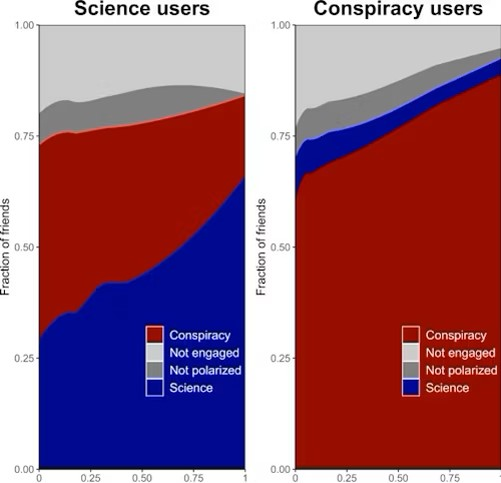
\includegraphics[width=\linewidth]{images/echo_chamber_graph_a.jpg}
		\caption{Gráfico demonstra câmara de eco entre usuários que seguem páginas de Ciência vs. Conspiraçao no Facebook e como nichos se afunilam promovendo isolamento entre usuários.}
		\fdireta{2019_Brugnoli}
		\label{fig:echo_chamber_graph_a}
	\end{subfigure}
	\hfill
	\begin{subfigure}{0.3\textwidth}
		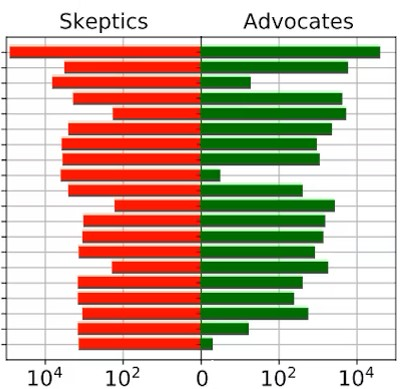
\includegraphics[width=\linewidth]{images/echo_chamber_graph_b.jpg}
		\caption{Gráfico demonstra a câmara de eco entre Céticos vs. Defensores da vacinação na Itália e como a polarização pode contribuir para a desinformação.}
		\fdireta{2020_Cossard}
		\label{fig:echo_chamber_graph_b}
	\end{subfigure}
	\hfill
	\begin{subfigure}{0.3\textwidth}
		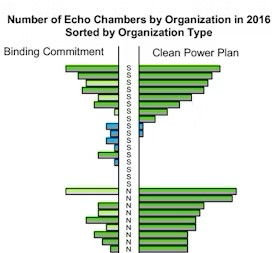
\includegraphics[width=\linewidth]{images/echo_chamber_graph_c.jpg}
		\caption{Grafico demonstra câmara de eco entre organicações no debate de políticas públicas de meio ambiente e mudanças climáticas dos EUA em 2016, especificamente sobre investir ou não em um plano de energia limpa.}
		\fdireta{2018_Jasny}
		\label{fig:echo_chamber_graph_c}
	\end{subfigure}
	\caption{Gráficos de polarização em estudos de análise de câmaras de eco.}
	\label{fig:echo_chamber_graph}
\end{figure}

Essa formação de grupos ideológicos não é meramente um reflexo da natureza humana, mas é intensificada pela arquitetura e algoritmos das plataformas digitais. Na busca por otimizar a experiência do usuário, essas plataformas frequentemente reforçam crenças preexistentes, gerando 'bolhas de filtro', conforme observado por \citeonline{2016_Flaxman}. Essas bolhas, embora possam servir como escudos contra informações perturbadoras, também restringem a exposição a uma gama diversificada de perspectivas. No entanto, a era digital não se resume apenas a câmaras de eco. \citeonline{2019_Brugnoli} destaca que em ambientes online, mecanismos cognitivos, como a evitação de desafio, viés de confirmação, dissonância cognitiva e a busca por validação, são intensificados, com a validação frequentemente a um clique de distância. Essa noção, reforça papel das mídias sociais na formação e reforço dessas fenômenos no ciberespaço.

\begin{citacao}
	'Eu defino o ciberespaço como o espaço de comunicação aberto pela interconexão mundial dos computadores e das memórias dos computadores. Essa definição inclui o conjunto dos sistemas de comunicação eletrônicos (aí incluídos os conjuntos de redes hertzianas e telefônicas clássicas), na medida em que transmitem informações provenientes de fontes digitais ou destinadas à digitalização. Insisto na codificação digital, pois ela condiciona o caráter plástico, fluido, calculável com precisão e tratável em tempo real, hipertextual, interativo e, resumindo, virtual da informação que é, parece-me, a marca distintiva do ciberespaço' \cite[p. 102]{2010_Levy_BOOK}.
\end{citacao}

\citeonline{{2010_Levy_BOOK}}, por sua vez, argumenta que as dinâmicas 'entrelaçadas' do ciberespaço refletem uma confluência de atores, projetos e interpretações, muitas vezes em oposição. O autor salienta que, apesar das tendências dominantes da era digital, a manifestação dessas tendências na vida cotidiana é multifacetada. A diversidade de interesses e perspectivas é emblemática da natureza fluida do ciberespaço. Enquanto alguns enxergam o ciberespaço como um domínio de comunicação livre e comunitária, outros o veem como um mercado global expansivo. Essas visões frequentemente colidem, ilustrando a complexidade e diversidade de vozes no ciberespaço. O autor também enfatiza que a representatividade cultural no ciberespaço é proporcional ao engajamento ativo e à qualidade das contribuições de seus participantes. Embora existam obstáculos à expressão da diversidade cultural, eles são menos proeminentes no ciberespaço do que em outros meios. Isso sugere que o ciberespaço, ao conectar indivíduos de diferentes origens, amplifica a diversidade de perspectivas. Em resumo, \citeonline{{2010_Levy_BOOK}} oferece uma perspectiva equilibrada e otimista sobre polarização e diversidade no ciberespaço. Ele reconhece os desafios da coexistência de múltiplas perspectivas, mas também vê o ciberespaço como um meio de expressão da diversidade cultural e colaboração. Isso sugere que, embora a polarização seja uma realidade, o ciberespaço também oferece oportunidades para diálogo e colaboração.

No contexto das plataformas digitais, a perspectiva de Lévy sobre a cibercultura é essencial para entender a dinâmica da polarização. Enquanto plataformas como o Colab podem enfrentar desafios de 'bolhas de filtro' que limitam a diversidade de perspectivas, a natureza interconectada da cibercultura, conforme descrito por Lévy, também apresenta oportunidades. Essa interconexão pode facilitar diálogos construtivos e a negociação de diferentes pontos de vista. Portanto, ao reconhecer e valorizar essa diversidade, o Colab tem o potencial de se tornar um espaço inclusivo para o diálogo cidadão.A abordagem de Lévy sobre a cibercultura ressalta a natureza interconectada e a valorização da diversidade de perspectivas em discursos online evocam a utilização de heurísticas analíticas inovadoras que possam extrair informações estratégicas a partir dos dados de redes sociais. O Colab, além de ser um aplicativo e uma rede social de cidadania, pode ser classificado como um 'barômetro social hiperlocal'. Isso significa que, ao analisar postagens do ponto de vista de sentimentos e personas, é possível inferir a pressão social sobre determinados assuntos, relacionados a tipos específicos de eventos, de comunidades específicas em locais específicos. Assim, o 'barômetro social hiperlocal' não é uma ferramenta separada, mas sim uma caracterização do próprio Colab e de sua capacidade de mediar e refletir as nuances das opiniões e sentimentos da comunidade.

Na análise sentimento e personas das postagens do usuários do Colab, uma tendência interessante se destaca: a maioria dos usuários foi classificado como \textit{helper}, com apenas alguns nichos dominados por \textit{complainers}. Esta classificação de personas proporciona entender de forma mais matizada da comunidade, destacando áreas de colaboração positiva e pontos de tensão. O conceito de 'barômetro social hiperlocal', aliado à análise de sentimentos das postagens, adiciona uma dimensão adicional ao nosso entendimento. Ao incorporar o tipo de evento como uma variável, podemos discernir nuances na pressão social manifestada pelos usuários. Enquanto, em média, as postagens tendem a adotar um tom mais neutro, a análise focada em eventos específicos revela áreas de intensa polarização, permitindo-nos identificar e abordar tópicos de particular tensão dentro da comunidade. Com as abordagens e ferramentas certas, como aquelas inspiradas por Lévy e implementadas no Colab, há um potencial significativo para promover a participação cidadã, o engajamento e a construção de comunidades mais informadas e coesas.

\section{Dinâmicas de Pressão Social}

A análise das interações no Colab revela uma rica dinâmica de participação cidadã em eventos de zeladoria pública. Com um total de 132.858 eventos registrados, observa-se uma participação ativa de 4.569 usuários únicos, indicando uma média de aproximadamente 29 eventos por usuário. Esta média sugere um engajamento considerável dos cidadãos na plataforma, refletindo sua preocupação e envolvimento ativo em questões de zeladoria em suas comunidades.

Ao explorar a estrutura de relacionamentos entre os usuários, identificamos 25.785 conexões, ou arestas, que delineiam a rede de interações no Colab. Estas arestas representam as conexões estabelecidas entre os 6.904 nós, ou entidades, que compõem a rede. Estes nós, em sua maioria, representam os usuários e suas características demográficas e geográficas.

Em relação à distribuição geográfica, Niterói emerge como a cidade com a maior representação, contabilizando 4.246 usuários. Em seguida, temos Santo André com 1.942 usuários e Mesquita com 716. No entanto, ao analisar a distribuição de eventos por cidade, observamos uma dinâmica interessante. Mesquita, apesar de ter o menor número de usuários, lidera em termos de eventos registrados, com um total de 63.927. Niterói, com o maior número de usuários, registra 42.191 eventos, enquanto Santo André contabiliza 26.740 eventos. Esta discrepância entre o número de usuários e o número de eventos sugere variações no nível de atividade e engajamento dos usuários em diferentes cidades.

A análise dos tipos de eventos reportados nas três cidades - Mesquita, Niterói e Santo André - revela padrões distintos de preocupações e demandas dos cidadãos em cada localidade, refletindo as particularidades e desafios urbanos enfrentados por cada comunidade.

\begin{figure}[htb]
	\centering
	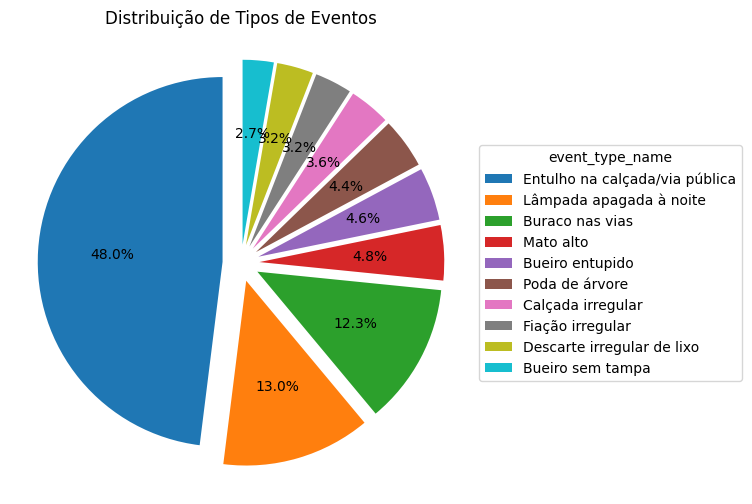
\includegraphics[width=0.7\textwidth]{images/pie_event_distribution.png}
	\caption{Distribuição dos tipos de evento mais comuns em Mesquita, Niterói e Santo André.}
	\label{fig:pie_event_distribution}
\end{figure}

Em Mesquita, o evento mais reportado, com uma expressiva quantidade de 45.235 registros, é 'Entulho na calçada/via pública'. Este número elevado sugere que a gestão de resíduos e a limpeza urbana são desafios significativos para a cidade. A presença massiva de entulho nas vias pode indicar problemas na coleta regular de lixo ou na conscientização da população sobre o descarte adequado. Além disso, eventos como 'Bueiro entupido' e 'Esgoto a céu aberto' também figuram no top 10. reforçando a ideia de que a infraestrutura urbana e os serviços de saneamento são áreas de preocupação para os cidadãos de Mesquita.

Por outro lado, em Niterói, a principal preocupação está relacionada à iluminação pública, com 'Lâmpada apagada à noite' liderando a lista. Este tipo de evento, além de estar relacionado à segurança pública, também pode afetar a qualidade de vida dos cidadãos, uma vez que áreas mal iluminadas podem desencorajar atividades noturnas e a circulação de pessoas. Adicionalmente, 'Buraco nas vias' e 'Fiação irregular' também são frequentemente reportados, indicando possíveis desafios na manutenção das vias públicas e na infraestrutura elétrica da cidade.

Em Santo André, 'Buraco nas vias' lidera as preocupações, seguido por eventos relacionados à gestão de resíduos e manutenção de áreas verdes, como 'Entulho na calçada/via pública' e 'Poda de árvore'. Estes dados sugerem que, embora haja preocupações com a infraestrutura viária, também existe uma demanda significativa por espaços urbanos mais verdes e bem cuidados.

\begin{figure}[htb]
	\centering
	\caption{10 Principais Tipos de Eventos mais criados por Cidade}\label{fig:city-events}
	\begin{subfigure}[b]{0.317\textwidth}
		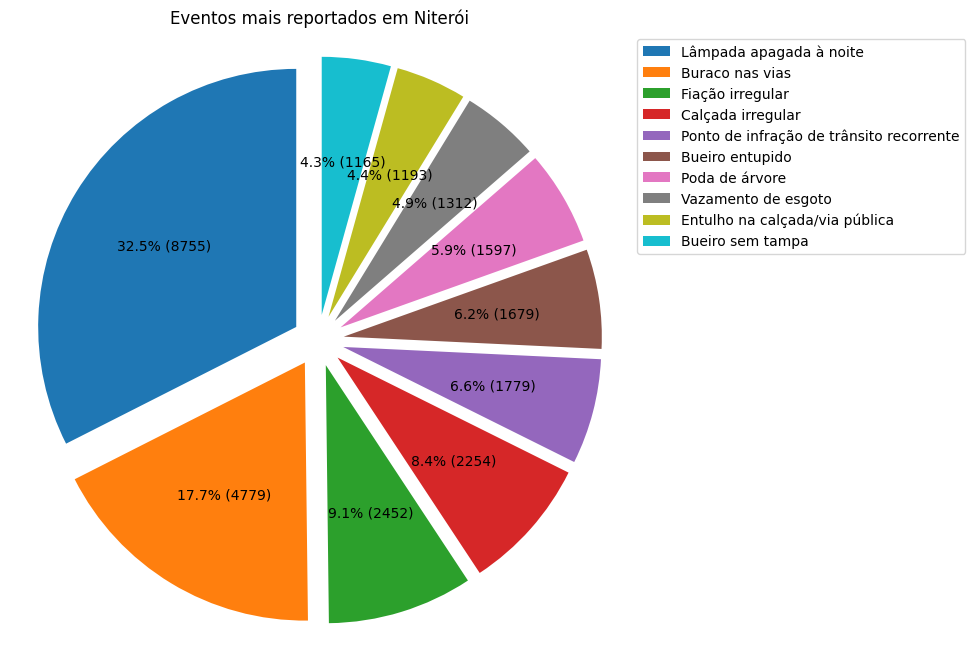
\includegraphics[width=\textwidth]{images/pie_event_distribution_niteroi.png}
		\caption{Niterói}
		\label{fig:niteroi-pie}
		\subcaption*{Em Niterói, o alto número de relatos sobre problemas como \textit{Lâmpada apagada à noite} e \textit{Buraco nas vias} pode indicar uma preocupação com a segurança noturna e a qualidade das estradas. A alta frequência desses eventos sugere a necessidade de intervenções específicas.}
	\end{subfigure} ~
	\begin{subfigure}[b]{0.317\textwidth}
		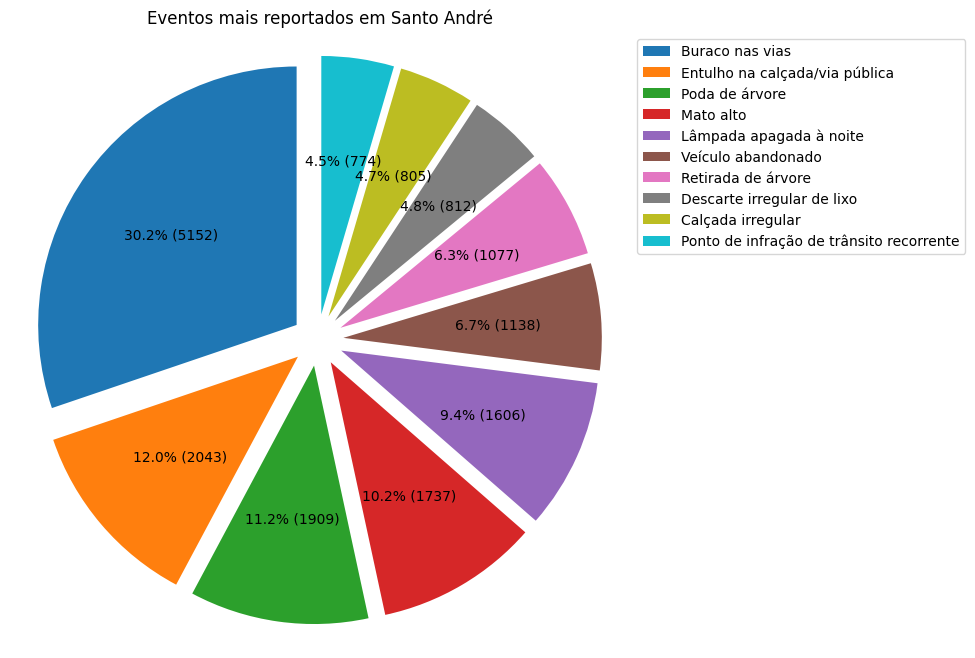
\includegraphics[width=\textwidth]{images/pie_event_distribution_sa.png}
		\caption{Santo André}
		\label{fig:santo-andre-pie}
		\subcaption*{Santo André destaca-se pela quantidade significativa de relatos sobre \textit{Buraco nas vias} e \textit{Entulho na calçada/via pública}. Esses problemas podem impactar a mobilidade urbana e a limpeza das áreas públicas. Talvez medidas de manutenção e limpeza sejam necessárias.}
	\end{subfigure} ~
	\begin{subfigure}[b]{0.317\textwidth}
		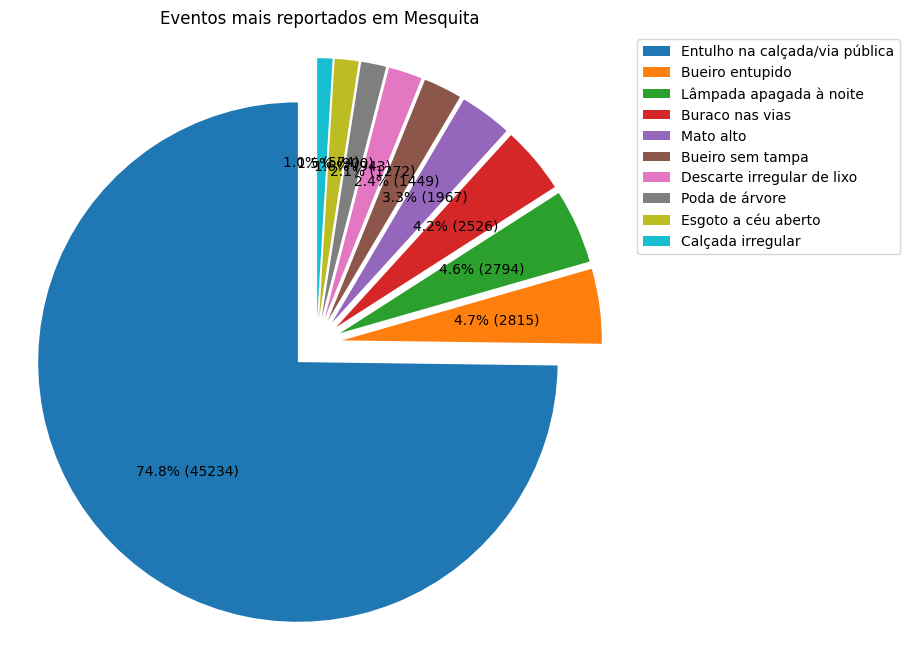
\includegraphics[width=\textwidth]{images/pie_event_distribution_mesquita.png}
		\caption{Mesquita}
		\label{fig:mesquita-pie}
		\subcaption*{Mesquita é caracterizada por um grande número de relatos sobre \textit{Entulho na calçada/via pública}, sugerindo uma preocupação com a limpeza em espaços públicos. A alta incidência desse problema pode indicar a necessidade de iniciativas de limpeza e conscientização.}
	\end{subfigure}
\end{figure}


Estas variações nas principais preocupações reportadas em cada cidade refletem a diversidade de desafios urbanos enfrentados por diferentes comunidades. A pressão social, como medida pela frequência e tipo de eventos reportados, serve como um indicativo das áreas que requerem atenção prioritária das autoridades locais. Ao mesmo tempo, a capacidade dos cidadãos de reportar e categorizar eventos em plataformas como o Colab permite uma compreensão mais aprofundada das dinâmicas locais, oferecendo uma ferramenta valiosa para a tomada de decisões informadas.

Além disso, a análise desses eventos também pode fornecer insights sobre a eficácia das políticas públicas em vigor. Por exemplo, um aumento súbito no número de eventos relacionados a 'Buraco nas vias' após uma temporada de chuvas pode indicar a necessidade de melhorias na infraestrutura viária. Da mesma forma, um número elevado de reportagens sobre 'Entulho na calçada/via pública' pode sinalizar a necessidade de campanhas de conscientização sobre descarte adequado ou de melhorias nos serviços de coleta de resíduos.

\section{Heurísticas para cálculo da Pressão Social Hiperlocal}

Nesta seção, abordaremos as heurísticas desenvolvidas para quantificar a pressão ou polaridade dos discursos nas postagens de eventos de zeladoria pública no Colab. Estas heurísticas, originadas de uma combinação de literatura existente e insights práticos, se tornaram cruciais para entender a opinião média de um grupo de usuários sobre eventos específicos de zeladoria pública. Elas são essenciais para medir a pressão social em comunidades hiperlocais, fornecendo insights valiosos para tomadores de decisão, pesquisadores e outros stakeholders interessados em compreender as complexas dinâmicas urbanas.

A relevância dessas heurísticas reside na sua capacidade de capturar a essência das opiniões dos cidadãos em contextos urbanos específicos. Ao analisar os tipos de eventos e as dinâmicas de participação cidadã na plataforma, podemos identificar tendências, preocupações e áreas de interesse, auxiliando na tomada de decisões informadas.

O conjunto de dados utilizado para esta análise foi meticulosamente compilado. Identificamos todos os usuários que fazem parte das comunidades da rede, conforme detalhado no \autoref{chapter:06_exploratory}, das cidades de Niterói, Santo André e Mesquita na rede Colab. Posteriormente, todas as postagens disponíveis desses usuários em eventos de zeladoria pública foram analisadas. Utilizamos o modelo de classificação descrito no \autoref{chapter:07_sentiment} para prever a persona do usuário e atribuir um score de sentimento a cada postagem. Esta metodologia nos permitiu obter insights sobre o comportamento dos usuários, como a expressão de suas opiniões e sentimentos. Adicionalmente, categorizamos os tipos de eventos associados a cada postagem.

\begin{table}[htbp]
	\centering
	\caption{Modelo de Dados para Análise de Pressão Social Hiperlocal}
	\begin{tabular}{ll}
		\toprule
		\textbf{Campo}    & \textbf{Descrição}                                  \\
		\midrule
		event\_id         & Identificador único do evento                       \\
		colab\_user\_id   & Identificador único do usuário do Colab             \\
		score             & Score de sentimento atribuído à postagem do usuário \\
		persona\_value    & Persona prevista para o usuário que fez a postagem  \\
		event\_type\_id   & Identificador único do tipo de evento               \\
		event\_type\_name & Nome descritivo do tipo de evento                   \\
		\bottomrule
	\end{tabular}
	\label{tab:modelo-dados-barometro}
\end{table}

Na \autoref{tab:modelo-dados-barometro}, cada linha representa uma postagem no Colab e inclui informações como o ID do evento, o ID do usuário do Colab, a pontuação de sentimento associada à postagem, a persona atribuída ao usuário que a fez, o ID do tipo de evento e o nome do tipo de evento relacionado. Esses dados formam a base essencial para nossas análises, permitindo-nos calcular a pressão social hiperlocal e compreender as dinâmicas das preocupações urbanas nessas comunidades específicas.

Com base neste modelo de dados, iniciamos o processo de filtragem e agregação. Primeiro, focamos nos membros ativos das comunidades identificadas na análise exploratória conduzida no \autoref{chapter:06_exploratory}. Em seguida, selecionamos tipos de eventos específicos, agrupados por tema, para nossa análise. Esta seleção foi guiada pela intenção de avaliar a pressão social hiperlocal em relação a preocupações específicas de zeladoria pública. Após a filtragem, calculamos duas métricas-chave para cada tipo de evento: a pontuação média de sentimento e a persona média. A primeira reflete o sentimento médio das postagens, enquanto a segunda representa a distribuição média das personas dos usuários. Essas métricas são calculadas para cada tipo de evento, permitindo-nos comparar e analisar as diferenças entre eles.

A visualização da pressão social hiperlocal é apresentada através de um gráfico de radar, uma representação gráfica que permite analisar e comparar diversas variáveis em relação a um ponto central. O gráfico possui dois planos distintos: o plano de score e o plano de persona.

\begin{figure}[htb]
	\centering
	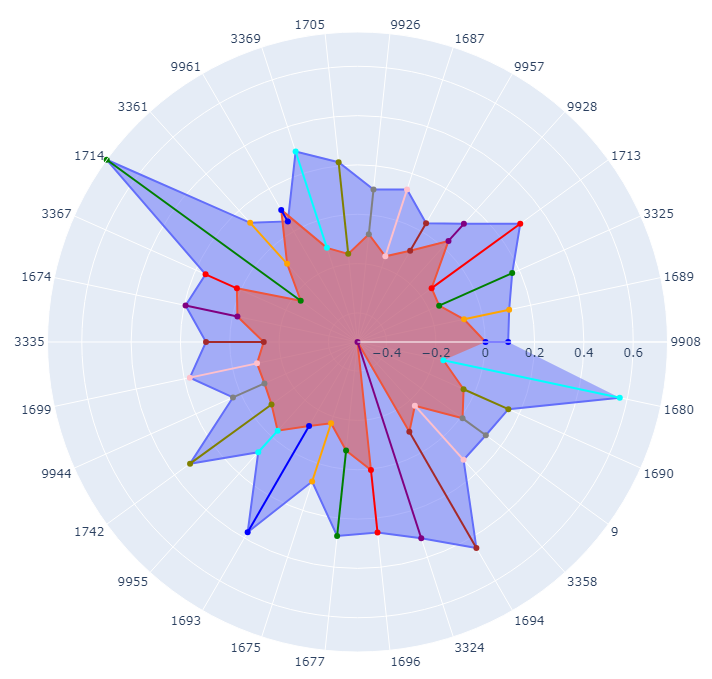
\includegraphics[width=0.7\textwidth]{images/social_barometer_plot.png}
	\caption{Gráfico de Radar para Análise de Pressão Social Hiperlocal. Os segmentos representam tipos de eventos, enquanto o eixo radial exibe valores médios de scores de sentimentos (plano vermelho) e personas (plano azul) atribuídos às postagens dos usuários relacionadas a cada tipo de evento.}
	\label{fig:social_barometer_plot}
\end{figure}

No plano de score, cada segmento do gráfico de radar representa um tipo específico de evento do Colab, onde cada evento é associado a um ângulo theta. O eixo radial, representado pelo parâmetro 'R', indica o valor médio dos scores de sentimentos atribuídos às postagens dos usuários em relação a um determinado tipo de evento. Quanto mais distante do centro estiver um segmento, maior será o valor médio do score e, consequentemente, mais positivo será o sentimento expresso pelos usuários em relação a esse evento. Por outro lado, segmentos mais próximos do centro indicam scores médios mais baixos, refletindo sentimentos mais negativos.

No plano de persona, novamente, cada segmento do gráfico representa um tipo de evento, O eixo radial 'R' neste caso indica o valor médio das personas previstas dos usuários em relação ao tipo de evento. Quanto mais próximo de 0 estiver um segmento, mais os usuários tendem a assumir uma persona de \textit{helper}, caracterizada por atitudes positivas e colaborativas em relação ao evento. À medida que o valor de 'R' se aproxima de 1, os usuários tendem a adotar uma persona de \textit{complainer}, indicando uma postura mais crítica e insatisfeita. Essa representação gráfica única proporciona uma visão abrangente e comparativa das opiniões e personas dos usuários do Colab em relação a diferentes tipos de eventos, permitindo uma análise mais profunda das dinâmicas das comunidades hiperlocais.

Após a definição do modelo de dados e a coleta das postagens no Colab, começamos a formulação das heurísticas que conduziriam à análise da pressão social hiperlocal. Esta etapa foi crucial, pois a vastidão e variedade dos dados requeriam um direcionamento para captar efetivamente as nuances das dinâmicas urbanas. O primeiro passo foi a identificação dos tópicos de interesse. Escolhemos tópicos que são comumente discutidos em comunidades urbanas e têm um impacto direto na qualidade de vida dos cidadãos. Um exemplo elucidativo dessa seleção é o tópico 'Tarifa de Transporte Público'. A escolha desse tema não se deu apenas pela sua manifesta relevância em discussões urbanas e pelo impacto direto que exerce no cotidiano financeiro e rotineiro dos cidadãos, mas também por sua ressonância histórica. Na história recente do Brasil, podemos remeter a um período de turbulência política, cujo estopim foi justamente o descontentamento popular em relação ao aumento das tarifas de transporte. Em junho de 2013, uma série de protestos, inicialmente convocados contra o aumento das passagens, ganhou magnitude e se espalhou por diversas cidades do país. Rapidamente, as manifestações incorporaram uma variedade de pautas e descontentamentos, culminando em uma das maiores mobilizações populares das últimas décadas no Brasil. Esse evento histórico ilustra a capacidade do tema 'Tarifa de Transporte Público' de catalisar discussões mais amplas e mobilizar grandes contingentes da população em torno de demandas comuns.

Para cada tópico escolhido, definimos um conjunto de palavras-chave. Estas palavras-chave são termos ou expressões frequentemente associados ao tópico em questão. No caso do tópico 'Tarifa de Transporte Público', palavras como 'lotado', 'ônibus', 'metrô', 'tarifa' e 'aumento da tarifa' foram consideradas. Essas palavras-chave funcionam como um filtro inicial, permitindo-nos identificar postagens no Colab que possam estar relacionadas ao tópico em análise. Com as palavras-chave definidas, realizamos uma busca nas postagens para identificar os tipos de eventos associados a elas. Esta busca retorna uma variedade de eventos, que podem ou não estar diretamente relacionados ao tópico de interesse.

Por exemplo, uma postagem que menciona 'passagem está cara' em um contexto de 'ônibus danificado' sugere uma intersecção do tópico de 'Tarifa de Transporte Público' com um evento relacionado. Isso indica que o usuário está manifestando sua insatisfação com o serviço, relacionando o valor pago à qualidade recebida. Para refinar ainda mais nossa análise, criamos uma lista de eventos não relevantes, que são excluídos da análise final. Esta lista foi elaborada com base em nossa compreensão do tópico e na intuição de quais eventos poderiam desviar o foco da pressão social que queríamos captar. No exemplo anterior, os eventos como 'Ponto de infração de trânsito recorrente' e 'Rampa de acessibilidade irregular ou inexistente' foram considerados na análise, pois, mesmo não sendo diretamente sobre tarifas, são eventos que afetam a experiência do usuário no transporte público.

Após a filtragem e seleção, calculamos métricas para os eventos restantes, como pontuação média de sentimento e persona média. A combinação dessas métricas, associadas aos eventos filtrados, nos fornece um panorama da pressão social em relação ao tópico analisado. Essa abordagem, que combina a seleção de tópicos, identificação por palavras-chave e filtragem de eventos, permite-nos isolar e analisar os sentimentos e opiniões dos usuários em relação a questões urbanas específicas, proporcionando insights valiosos sobre as dinâmicas das comunidades urbanas.

\section{Tópicos de Pressão Social}

O Colab é uma plataforma de participação cidadã que proporciona um espaço virtual para os cidadãos expressarem suas preocupações, compartilharem experiências e debaterem questões urbanas relevantes. Neste ambiente, emergem tópicos de pressão social que refletem as preocupações específicas dos cidadãos. A escolha desses tópicos foi baseada não apenas na sua frequência de aparição na plataforma, mas também na sua relevância para as políticas públicas urbanas e na amplitude de impacto que podem ter nas comunidades. Ao escolher esses tópicos, procuramos abordar tanto questões mais generalizadas, como saúde e segurança, quanto questões emergentes e altamente debatidas, como gentrificação e higienismo social. Esses tópicos desempenham um papel fundamental na compreensão dos desafios enfrentados nas cidades. Em uma plataforma como o Colab, as preocupações dos cidadãos podem ser expressas de maneira apaixonada e, por vezes, polarizada. Através de uma busca por palavras-chave específicas, identificamos e categorizamos diversos desses tópicos de pressão social que surgem nas discussões e associamos eventos de zeladoria pública a esses tópicos. Agora, nosso objetivo é analisar esses tópicos sob a perspectiva do Colab como um 'Barômetro Social Hiperlocal', investigando como eles impactam a dinâmica da plataforma e fornecem informações valiosas para decisores, pesquisadores e comunidades e munícipes.

\subsection{Mobilidade Urbana}

A mobilidade urbana é um tema de crescente importância no contexto das cidades modernas, à medida que as populações urbanas continuam a crescer e as infraestruturas de transporte enfrentam desafios cada vez maiores. No ambiente colaborativo do Colab, onde cidadãos compartilham suas experiências e preocupações sobre a vida urbana, a mobilidade é um tópico central de discussão. A era das 'smart cities' e dos 'connected citizens' trouxe consigo uma série de inovações e tecnologias que prometem melhorar a mobilidade nas cidades, mas também desencadeou debates apaixonados sobre o futuro da mobilidade urbana.

\begin{figure}[htb]
	\centering
	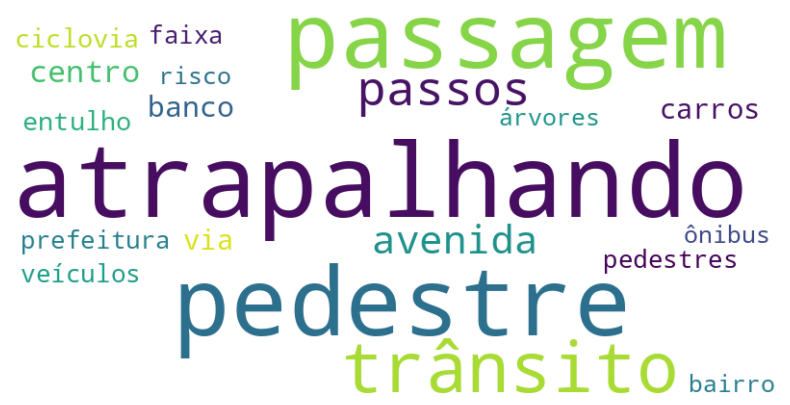
\includegraphics[width=0.7\textwidth]{images/wordcloud_mobility.png}
	\caption{Wordcloud com palavras mais frequentes em postagens sobre mobilidade urbana}
	\label{fig:wordcloud_mobility}
\end{figure}

A polarização em torno da mobilidade urbana pode ser observada em várias frentes. Uma das fontes mais comuns de polarização é a preferência por diferentes modos de transporte. Alguns cidadãos podem advogar veementemente pelo uso de veículos particulares e pela expansão das vias expressas, enquanto outros defendem o transporte público, ciclovias e pedestrianismo como soluções mais sustentáveis. Essa divergência de opiniões pode levar a debates acalorados sobre como os recursos da cidade devem ser alocados.

Além disso, questões ambientais desempenham um papel fundamental na polarização da mobilidade urbana. Aqueles que valorizam a redução das emissões de carbono e a promoção de meios de transporte ecológicos, como veículos elétricos e bicicletas, frequentemente entram em conflito com aqueles que resistem a medidas que limitam o uso de veículos particulares em nome do meio ambiente. Os debates relacionados a trânsito automobilistico são tão frequentes quanto os debates que advogam por mais ciclovias e meios alternativos de transporte. A acessibilidade e a equidade também são fontes de divisão. Garantir que todos os cidadãos tenham acesso aos sistemas de transporte público é uma preocupação importante, mas as decisões sobre como alcançar essa equidade podem ser polarizantes. Outro ponto de discórdia é o planejamento urbano. Decisões sobre a criação de ciclovias, expansão do transporte público e medidas para lidar com o congestionamento de tráfego frequentemente dividem as opiniões dos cidadãos. Alguns veem essas mudanças como melhorias na qualidade de vida, enquanto outros as percebem como inconvenientes ou dispendiosas.

\begin{figure}[htb]
	\centering
	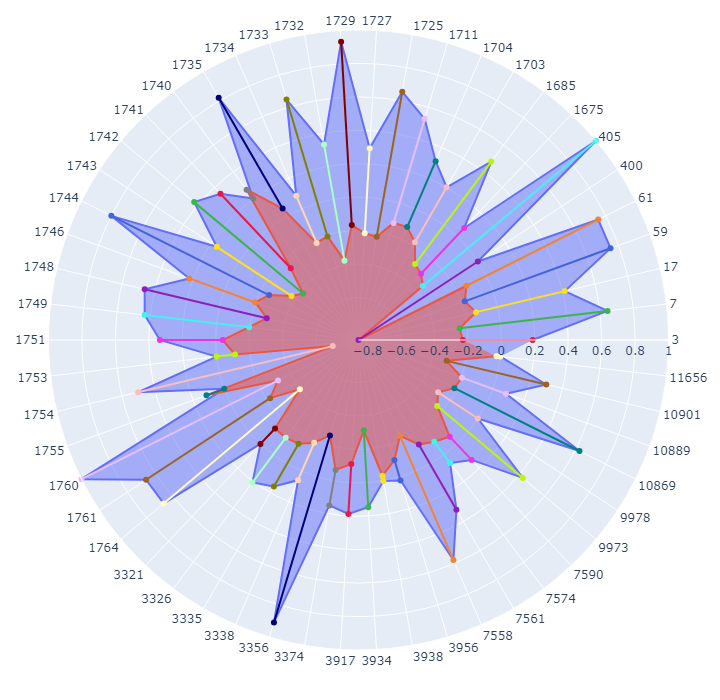
\includegraphics[width=0.7\textwidth]{images/social_barometer_mobility.png}
	\caption{Gráfico de Radar ilustrando a pressão social em relação à mobilidade urbana. O eixo radial mostra os scores de sentimentos (plano vermelho) e personas (plano azul), enquanto os segmentos descrevem diversos eventos urbanos.}
	\label{fig:social_barometer_mobility}
\end{figure}

\begin{table}[htbp]
	\centering
	\caption{Métricas de pressão social do tópico de Mobilidade Urbana}
	\label{tab:eventos_populares_mobility}
	\begin{tabular}{|l|c|c|c|c|}
		\hline
		\textbf{Tipo de Evento}                         & \textbf{Eventos} & \textbf{Score} & \textbf{Persona} \\
		\hline
		1725:Bloqueio na via                            & 16               & -0.2272        & 0.6535           \\
		\hline
		7:Ponto de infração de trânsito recorrente      & 16               & -0.2458        & 0.6454           \\
		\hline
		3:Buraco nas vias                               & 15               & -0.2305        & 0.1872           \\
		\hline
		3938:Entulho na calçada/via pública             & 13               & -0.0303        & 0.0022           \\
		\hline
		7561:Ponto de alagamento                        & 11               & -0.1329        & 0.3171           \\
		\hline
		7558:Ocupação irregular de área pública         & 11               & -0.2296        & 0.5789           \\
		\hline
		1727:Equipamento público danificado             & 11               & -0.2151        & 0.2941           \\
		\hline
		3917:Calçada irregular                          & 10               & -0.1119        & 0.1880           \\
		\hline
		1749:Manutenção de semáforo                     & 10               & -0.1963        & 0.4333           \\
		\hline
		3335:Lâmpada apagada à noite                    & 10               & -0.1377        & 0.1576           \\
		\hline
		1675:Bueiro sem tampa                           & 9                & -0.3101        & 0.0667           \\
		\hline
		1703:Ponto de travessia irregular               & 9                & -0.1792        & 0.2000           \\
		\hline
		1704:Calçada inexistente                        & 9                & -0.1193        & 0.3103           \\
		\hline
		1741:Manutenção de ciclovia/ciclofaixa          & 9                & -0.2643        & 0.3487           \\
		\hline
		1729:Ponto de transporte clandestino            & 8                & -0.1662        & 0.9333           \\
		\hline
		1711:Ponto de ônibus danificado                 & 8                & -0.1235        & 0.5263           \\
		\hline
		1734:Retirada de árvore                         & 8                & -0.2225        & 0.0847           \\
		\hline
		7574:Poda de árvore                             & 7                & -0.0959        & 0.0632           \\
		\hline
		10889:Placa de sinalização quebrada/inexistente & 7                & -0.1963        & 0.0843           \\
		\hline
		1733:Publicidade irregular em via pública       & 7                & -0.2081        & 0.6471           \\
		\hline
	\end{tabular}
\end{table}

Compreender as nuances da pressão social em comunidades hiperlocais é fundamental para visualizar e analisar as preocupações dos cidadãos em contextos urbanos específicos. Na plataforma Colab, os usuários têm a oportunidade de expressar seus sentimentos e opiniões sobre variados eventos de zeladoria pública. As heurísticas desenvolvidas, e o modelo de dados correspondente, oferecem uma estrutura valiosa para desvendar as complexidades desses discursos.

Ao observar os resultados de pressão social sobre mobilidade urbana, é possível identificar as áreas mais críticas e aquelas que possuem sentimentos mais positivos, bem como as que contam com um maior número de postagens. O 'Buraco nas vias', com 15 postagens, obteve um score de sentimento de -0.2308 e uma persona de 0.1889. Isto sugere um sentimento negativo, porém a persona indica uma tendência ligeiramente inclinada para o \textit{helper}, indicando que os usuários estão mais inclinados a ajudar ou colaborar para solucionar o problema, ao invés de apenas reclamar. Por outro lado, eventos como 'Ponto de infração de trânsito recorrente', com 16 postagens, demonstraram uma pontuação de sentimento de -0.2496 e uma persona de 0.6442. A pontuação de sentimento, sendo negativa, sugere insatisfação com o tópico. No entanto, a alta pontuação da persona revela que os usuários tendem a ser mais \textit{complainers} do que \textit{helper} nesse cenário.

Eventos como 'Rampa de acessibilidade irregular ou inexistente' e 'Estação de ônibus/trem/metrô danificada' tiveram menos postagens, mas ainda assim mostraram sentimentos negativos, ressaltando a necessidade de atenção a essas áreas. Por outro lado, temos tópicos como 'Via de terra com desnível' e 'Bicicletário/paraciclo danificado' que mostraram sentimentos ligeiramente positivos, com scores de 0.0533 e 0.2662 respectivamente. Isso poderia sugerir que, embora ainda haja problemas nestas áreas, houve algumas melhorias ou ações que foram bem recebidas pelos cidadãos. Os eventos mais populares, aqueles com o maior número de postagens, como 'Bloqueio na via' com 17 postagens, dão uma ideia clara sobre quais tópicos de mobilidade urbana são mais discutidos ou problemáticos nas comunidades abordadas.

A combinação de scores de sentimentos com valores de persona fornece uma visão holística. Por exemplo, um sentimento negativo associado a uma persona de \textit{helper} pode indicar um problema, mas também uma comunidade disposta a colaborar para soluções. Por outro lado, um sentimento negativo com uma persona de \textit{complainer} pode indicar insatisfação acentuada e uma percepção de que ações práticas não estão sendo tomadas para resolver problemas. Assim, ao analisar a pressão social em tópicos de mobilidade urbana, pode-se inferir quais áreas precisam de mais atenção e onde as administrações públicas podem focar seus esforços para melhorar a satisfação e o bem-estar dos cidadãos. Estes insights são valiosos para gestores urbanos, tomadores de decisão e pesquisadores, ajudando a moldar políticas públicas mais eficientes e a orientar futuras intervenções urbanas.

\subsection{Infrações de Trânsito}

No campo das infrações de trânsito, emerge um padrão intrigante na pressão social exercida pelos cidadãos urbanos. A análise dos dados oferece uma perspectiva única sobre a maneira como os usuários percebem e reagem às ações (ou inações) das autoridades de trânsito. De acordo com as informações disponíveis, há uma dicotomia clara em relação à maneira como as autoridades de trânsito são percebidas. Por um lado, percebe-se uma sensação predominante de que as autoridades poderiam estar fazendo mais para resolver as infrações, enquanto, por outro lado, alguns usuários percebem as autoridades como parte de uma 'indústria da multa', sugerindo um excesso de penalidades.

Um olhar atento às palavras-chave associadas ao tópico revela que 'multa' é a palavra mais mencionada, seguida por 'infração', indicando que a principal preocupação dos cidadãos gira em torno das penalidades e das regras de trânsito. Além disso, a menção de termos como 'detran' e 'IPVA' sugere questões burocráticas e fiscais que podem estar influenciando a forma como as infrações de trânsito são percebidas.

\begin{figure}[htb]
	\centering
	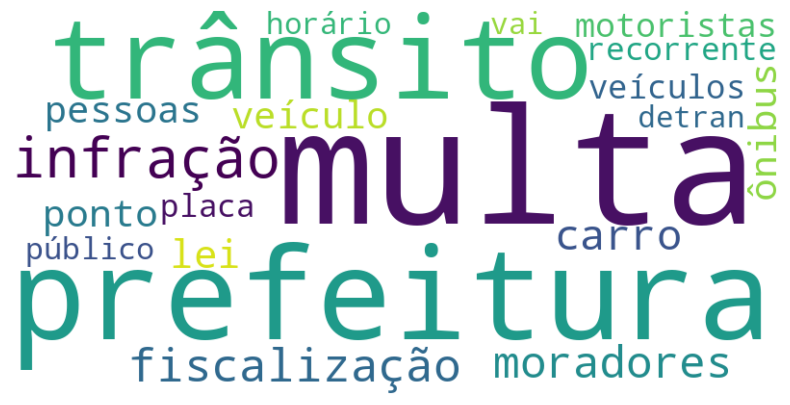
\includegraphics[width=0.7\textwidth]{images/wordcloud_traffic.png}
	\caption{Wordcloud com palavras mais frequentes em postagens sobre infrações de trânsito}
	\label{fig:wordcloud_traffic}
\end{figure}

Ao se aprofundar na análise da pressão social relacionada às infrações de trânsito, é evidente que as postagens dos cidadãos no Colab refletem uma diversidade de sentimentos e perspectivas. Observando inicialmente o score médio dos eventos, notamos que 'Via de terra com desnível' e 'Conservação (via pública)' são associados a sentimentos predominantemente positivos. Isso pode sugerir uma satisfação dos cidadãos com medidas tomadas em relação a essas questões específicas ou uma expressão de gratidão pelo reconhecimento de problemas solucionados. Em contrapartida, eventos como 'Manutenção de faixa de pedestre', 'Ônibus/trem/metrô danificado' e 'Manutenção de ciclovia/ciclofaixa' apresentam os scores mais negativos, indicando uma insatisfação ou preocupação dominante sobre esses tópicos.

Por outro lado, ao analisar a persona média atribuída aos usuários, percebemos que eventos como 'Rampa de acessibilidade irregular ou inexistente', 'Bueiro sem tampa', 'Calçada inexistente' e 'Publicidade irregular em via pública' têm uma persona média de 1.0. indicando uma predominância de \textit{complainers}. Isso sugere que os usuários, ao se depararem com esses problemas, mostram-se predominantemente críticos e insatisfeitos. Estas questões, aparentemente, tocam em aspectos sensíveis da comunidade, possivelmente relacionados à acessibilidade e segurança.

\begin{figure}[htb]
	\centering
	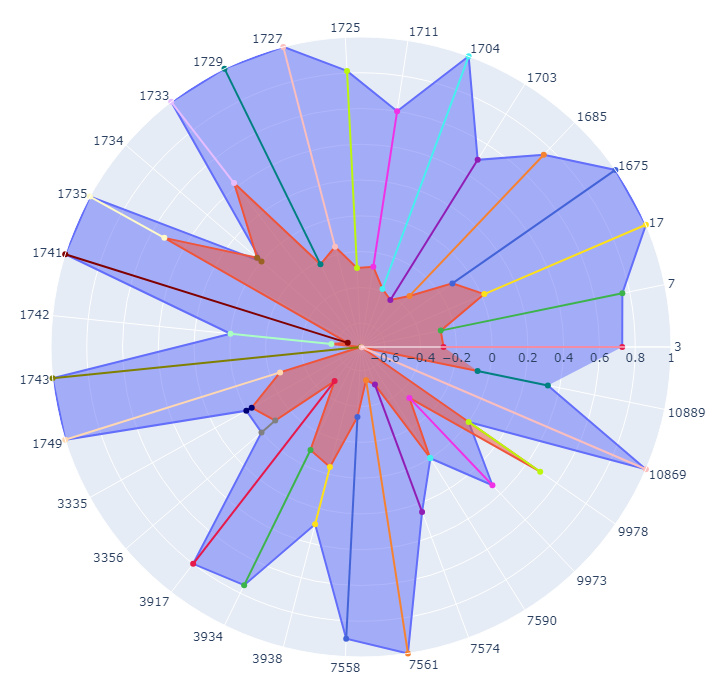
\includegraphics[width=0.7\textwidth]{images/social_barometer_traffic.png}
	\caption{Gráfico de Radar ilustrando a pressão social em relação ao tópico de Infrações de Trânsito.}
	\label{fig:social_barometer_traffic}
\end{figure}

\begin{table}[htbp]
	\centering
	\caption{Métricas de pressão social do tópico de Infrações de Trânsito}
	\label{tab:eventos_populares_traffic}
	\begin{tabular}{|l|c|c|c|c|}
		\hline
		\textbf{Tipo de Evento}                           & \textbf{Eventos} & \textbf{Score} & \textbf{Persona} \\
		\hline
		7:Ponto de infração de trânsito recorrente        & 4                & -0.2781        & 0.7586           \\
		\hline
		1685:Estabelecimento com acessibilidade irregular & 4                & -0.3392        & 0.7500           \\
		\hline
		3:Buraco nas vias                                 & 3                & -0.2719        & 0.7273           \\
		\hline
		3938:Entulho na calçada/via pública               & 3                & -0.0405        & 0.2903           \\
		\hline
		1725:Bloqueio na via                              & 3                & -0.2907        & 0.8125           \\
		\hline
		1727:Equipamento público danificado               & 3                & -0.1544        & 1.0000           \\
		\hline
		7590:Bueiro entupido                              & 2                & -0.0036        & 0.0000           \\
		\hline
		7574:Poda de árvore                               & 2                & -0.5093        & 0.2500           \\
		\hline
		7558:Ocupação irregular de área pública           & 2                & -0.3412        & 0.9000           \\
		\hline
		3917:Calçada irregular                            & 2                & -0.4922        & 0.8000           \\
		\hline
		3335:Lâmpada apagada à noite                      & 2                & -0.0344        & 0.0000           \\
		\hline
		1749:Manutenção de semáforo                       & 2                & -0.2593        & 1.0000           \\
		\hline
		10889:Placa de sinalização quebrada/inexistente   & 2                & -0.0677        & 0.3333           \\
		\hline
		1703:Ponto de travessia irregular                 & 2                & -0.4231        & 0.5000           \\
		\hline
		1675:Bueiro sem tampa                             & 2                & -0.1105        & 1.0000           \\
		\hline
		1711:Ponto de ônibus danificado                   & 2                & -0.2792        & 0.6000           \\
		\hline
		1735:Via de terra com desnível                    & 1                & 0.5242         & 1.0000           \\
		\hline
		10869:Ônibus/trem/metrô danificado                & 1                & -0.7298        & 1.0000           \\
		\hline
		9978:Conservação (via pública)                    & 1                & 0.4875         & 0.0000           \\
		\hline
		9973:Má conduta de motorista ou cobrador          & 1                & -0.3405        & 0.3333           \\
		\hline
	\end{tabular}
\end{table}

Em contraste, eventos como 'Retirada de árvore', 'Vazamento de esgoto', 'Poda de árvore', 'Bueiro entupido' e 'Conservação (via pública)' têm valores de persona tendendo a zero, o que implica uma predominância de usuários com a persona \textit{helper}. Esta constataçãos sugere que, para esses tópicos, os usuários tendem a adotar uma postura mais colaborativa, possivelmente oferecendo soluções, identificando problemas de maneira construtiva ou mesmo agradecendo por serviços realizados.

A presença significativa de palavras-chave como 'multa', 'infração', 'IPVA' e 'detran' nos resultados sugere que questões burocráticas e de regulamentação são temas recorrentes nas postagens. Este é um indicativo da preocupação dos cidadãos com o cumprimento das normas e com as consequências financeiras das infrações. Essas keywords podem ser um reflexo da percepção de que a gestão do trânsito e a aplicação das regras são cruciais para a qualidade de vida urbana.

Ao considerar a quantidade de postagens associadas a cada evento, nota-se que 'multa' e 'Ponto de infração de trânsito recorrente' são os mais citados, o que denota um alto nível de engajamento dos usuários com esses tópicos. Isso sugere que as multas e as zonas de infração recorrente são pontos de grande interesse e debate dentro da comunidade. A frequente menção a esses tópicos pode indicar tanto um reconhecimento dos problemas quanto uma busca por soluções e esclarecimentos.

As dinâmicas observadas na análise dos scores e das personas indicam que os cidadãos não apenas identificam problemas, mas também buscam engajamento ativo. Há uma interação contínua entre a crítica construtiva e a expressão de insatisfação. Esta interação reflete a natureza plural das preocupações urbanas e a complexidade das dinâmicas sociais em torno das infrações de trânsito.

O contraste entre os sentimentos positivos e negativos, assim como entre as personas \textit{helper} e \textit{complainer}, destaca a diversidade inerente na pressão social. Ela não se apresenta de forma uniforme, mas sim como um conjunto diversificado de vozes e perspectivas. Cada uma destas contribui para uma compreensão mais completa e detalhada dos desafios e necessidades das comunidades urbanas.

No discurso sobre infrações de trânsito, a pressão social revela complexidades nas percepções e sentimentos dos habitantes urbanos. A dissecção desses dados nos oferece uma lente pela qual podemos observar as nuances nas reações dos cidadãos às decisões das autoridades de trânsito. De acordo com os insights gerados, emerge uma dualidade perceptiva: muitos sentem que as autoridades poderiam ser mais proativas na solução de infrações, enquanto outros veem estas mesmas autoridades como propulsoras de uma 'indústria da infração', onde o foco estaria mais na penalização do que na resolução de problemas reais. A frequente menção a termos como 'multa', 'infração', 'detran' e 'IPVA' enfatiza as preocupações centrais dos cidadãos, as quais transcendem as penalidades e abarcam aspectos burocráticos e fiscais. Em síntese, ao decifrar a pressão social associada às infrações de trânsito, obtemos um mosaico rico em detalhes sobre as necessidades e inquietações de comunidades urbanas, fornecendo orientações valiosas para formuladores de políticas, acadêmicos e defensores do bem-estar urbano.

\subsection{Tarifa de Transporte Público}

A análise dos dados sobre pressão social no contexto da tarifa de transporte público evidencia a ampla preocupação dos cidadãos sobre esse tópico. O transporte público é um elemento fundamental da infraestrutura urbana e, como tal, tem implicações diretas na qualidade de vida dos habitantes de uma cidade. As keywords associadas a este tópico revelam preocupações específicas: o termo 'passagem', por exemplo, foi mencionado 11.593 vezes, destacando-se claramente como o ponto principal de discussão entre os usuários. Outras palavras-chave como 'ônibus', 'terminal' e 'cobertura' são também indicativas das discussões em torno do funcionamento e acessibilidade do transporte público.

\begin{figure}[htb]
	\centering
	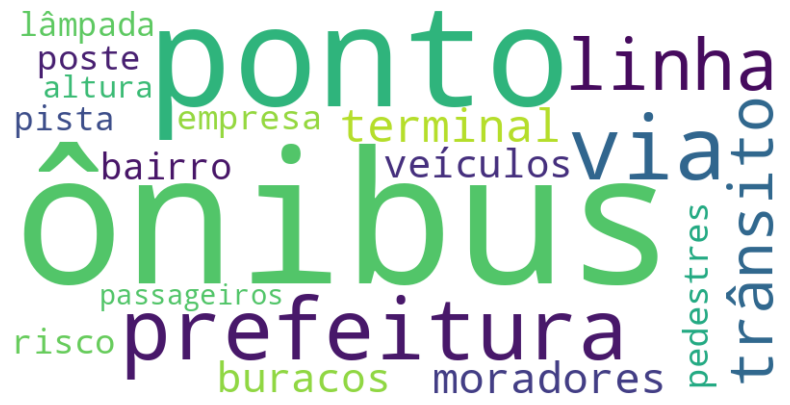
\includegraphics[width=0.6\textwidth]{images/wordcloud_busfare.png}
	\caption{Wordcloud com palavras mais frequentes em postagens sobre infrações de trânsito}
	\label{fig:wordcloud_busfare}
\end{figure}

Ao analisar os dados referentes ao tópico de pressão social relacionado à tarifa de transporte público, observou-se uma notável complexidade nas opiniões e sentimentos expressos pelos cidadãos. A estrutura deste tema, de relevância substancial para a vida diária das pessoas, possui nuances que precisam ser cuidadosamente interpretadas para se chegar a uma compreensão sólida.

Primeiramente, é notável que muitos dos eventos são fortemente relacionados a problemas percebidos no sistema de transporte público. Isso é evidente na menção a eventos como 'Ônibus superlotado', 'Ônibus fora do horário/rota' e 'Má conduta de motorista ou cobrador'. O score médio de sentimento atribuído a essas postagens é majoritariamente negativo, indicando insatisfação dos usuários. Além disso, a persona média associada a tais postagens, em sua maioria, inclina-se mais para o perfil de \textit{complainer}, sugerindo que os cidadãos estão expressando suas frustrações e preocupações em relação a esses problemas.

\begin{figure}[htb]
	\centering
	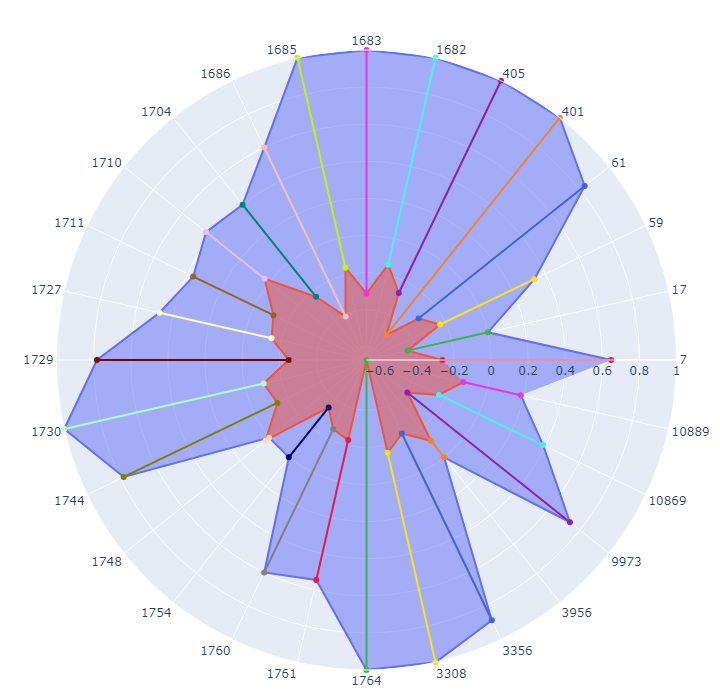
\includegraphics[width=0.7\textwidth]{images/social_barometer_bus_fare.png}
	\caption{Gráfico de Radar ilustrando a pressão social em relação ao tópico de Tarifa de Transporte Público}
	\label{fig:social_barometer_bus_fare}
\end{figure}

\begin{table}[htbp]
	\centering
	\caption{Métricas de pressão social do tópico de Transporte Público}
	\label{tab:eventos_populares_busfare}
	\begin{tabular}{|l|c|c|c|c|}
		\hline
		\textbf{Tipo de Evento}                              & \textbf{Eventos} & \textbf{Score} & \textbf{Persona} \\
		\hline
		1729:Ponto de transporte clandestino                 & 7                & -0.2516        & 0.7818           \\
		\hline
		3356:Ônibus fora do horário/rota                     & 7                & -0.2312        & 0.8861           \\
		\hline
		1727:Equipamento público danificado                  & 6                & -0.1464        & 0.4737           \\
		\hline
		9973:Má conduta de motorista ou cobrador             & 6                & -0.3900        & 0.7317           \\
		\hline
		10869:Ônibus/trem/metrô danificado                   & 5                & -0.2377        & 0.3855           \\
		\hline
		7:Ponto de infração de trânsito recorrente           & 5                & -0.2622        & 0.6483           \\
		\hline
		405:Ônibus superlotado                               & 5                & -0.2701        & 1.0000           \\
		\hline
		61:Ônibus/trem/metrô superlotado                     & 5                & -0.3126        & 0.8333           \\
		\hline
		59:Estação de ônibus/trem/metrô danificada           & 4                & -0.2304        & 0.3333           \\
		\hline
		1711:Ponto de ônibus danificado                      & 4                & -0.1144        & 0.3654           \\
		\hline
		1744:Ônibus danificado                               & 4                & -0.1378        & 0.7818           \\
		\hline
		1760:Estação de ônibus danificada                    & 4                & -0.2573        & 0.6000           \\
		\hline
		1683:Estabelecimento sem alvará                      & 3                & -0.3125        & 1.0000           \\
		\hline
		10889:Placa de sinalização quebrada/inexistente      & 2                & -0.1365        & 0.1818           \\
		\hline
		1685:Estabelecimento com acessibilidade irregular    & 2                & -0.1614        & 1.0000           \\
		\hline
		1704:Calçada inexistente                             & 2                & -0.2354        & 0.4000           \\
		\hline
		1710:Ponto de assalto/roubo                          & 2                & 0.0313         & 0.4348           \\
		\hline
		17:Rampa de acessibilidade irregular ou inexistente  & 2                & -0.4443        & 0.0000           \\
		\hline
		3956:Faixa de pedestre apagada                       & 2                & -0.1145        & 0.0000           \\
		\hline
		1761:Manutenção/implantação de infraestrutura viária & 2                & -0.2283        & 0.5455           \\
		\hline
	\end{tabular}
\end{table}

No entanto, ao observar eventos como 'Conservação (via pública)' e 'Faixa de pedestre apagada', nota-se que o sentimento médio expresso é menos negativo e a persona média tende mais ao perfil de \textit{helper}. Isso sugere que, embora os usuários estejam destacando questões que necessitam de atenção, há uma disposição para colaborar e auxiliar na resolução destes problemas. Esta dicotomia entre crítica e disposição para ajudar é fundamental para compreender as dinâmicas de pressão social em relação ao transporte público.

Dentro desta análise, um dos insights mais marcantes refere-se à relevância das palavras-chave identificadas. O termo 'ônibus' aparece com destaque, enquanto 'metrô' tem uma ocorrência muito mais rara. Isso sugere que os problemas associados aos ônibus podem ser mais prevalentes ou, pelo menos, mais reportados pelos usuários. Além disso, o termo 'passagem' foi mencionado com extraordinária frequência, indicando a centralidade deste tema no discurso dos cidadãos sobre o transporte público. A presença dominante deste termo pode ser interpretada como uma expressão de preocupação em relação aos custos e acessibilidade do transporte.

Quando se considera eventos com descrições como 'Agentes e Operadores de trânsito' ou 'Metrô/trem danificado', é evidente que a persona prevalece como \textit{complainer}, com scores de sentimentos decididamente negativos. Essa informação é vital para as partes interessadas, como governos locais e operadoras de transporte, pois destaca áreas específicas de preocupação que podem requerer ações imediatas.

Em contrapartida, eventos como 'Manutenção de pintura da via' e 'Banco danificado' apresentaram personas predominantemente \textit{helper}, mesmo que o número de postagens seja limitado. Isso pode sinalizar que, em certos contextos, os cidadãos estão mais inclinados a colaborar e oferecer feedback construtivo do que apenas expressar descontentamento. Ao avaliar a distribuição e intensidade dos scores de sentimento e personas em eventos diversos, torna-se evidente que o tópico de tarifa de transporte público não é apenas uma área de contenda, mas também de colaboração. A polarização entre os sentimentos positivos e negativos sugere que, enquanto existem desafios significativos a serem abordados, também há um potencial considerável para envolver os cidadãos na busca de soluções.

\subsection{Saúde Pública}

A saúde pública é indiscutivelmente um tópico de grande relevância para as comunidades, e os dados fornecidos corroboram essa assertividade. Ao analisar as palavras-chave relacionadas ao tópico de saúde pública, notamos termos como 'samu', 'ambulância', 'médico' e 'vacina', que são elementos essenciais no contexto de serviços de saúde. Além disso, a menção a doenças como 'dengue' e 'zika', e a presença significativa desses termos, sinaliza uma preocupação com problemas de saúde emergentes e potencialmente perigosos.

Outra observação crucial é a relação de tipos de eventos associados a este tópico. Nota-se que eventos como 'Foco de mosquito da dengue/zika' e 'Mato alto' aparecem com frequência, o que pode indicar problemas relacionados ao meio ambiente e ao controle de vetores de doenças. O 'Descarte irregular de lixo' também surge como um evento relevante, refletindo questões sanitárias e a preocupação da comunidade com a limpeza pública e seus impactos na saúde coletiva.

\begin{figure}[htb]
	\centering
	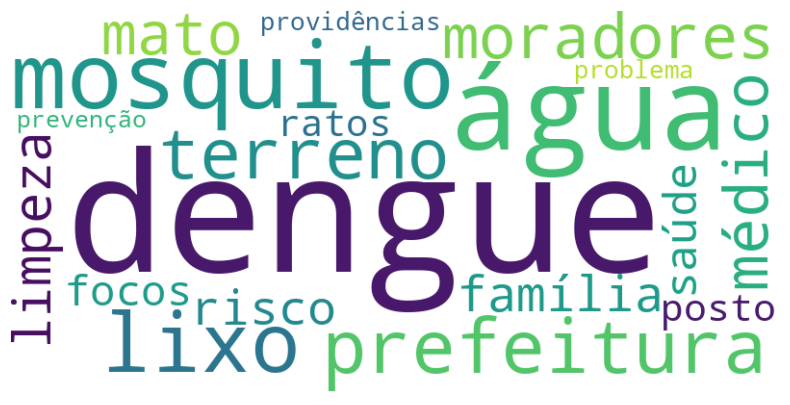
\includegraphics[width=0.7\textwidth]{images/wordcloud_public_health.png}
	\caption{Wordcloud com palavras mais frequentes em postagens sobre Saúde Pública}
	\label{fig:wordcloud_public_health}
\end{figure}

A análise da pressão social em relação à saúde pública nas plataformas do Colab revelou diversas nuances sobre a percepção cidadã concernente à zeladoria urbana neste tema. Inicialmente, ao observar o gráfico de radar, é possível notar que certos tipos de eventos possuem sentimentos majoritariamente negativos, indicados por scores abaixo de zero, enquanto outros se aproximam de um sentimento mais neutro ou até mesmo positivo.

O evento denominado 'Ponto recorrente de poluição sonora' apresentou uma média de sentimento negativa e uma persona média indicando uma predominância do tipo \textit{complainer}. Isso sugere uma insatisfação marcante dos usuários do Colab em relação a esse problema específico, destacando a urgência na busca por soluções eficazes para tal questão. Uma hipótese para esta situação pode ser a percepção direta dos efeitos da poluição sonora na qualidade de vida, levando a uma reação mais negativa por parte dos cidadãos.

Por outro lado, ao analisar o evento 'Descarte irregular de lixo', foi observado um sentimento médio negativo, mas uma persona média de 0.4783, o que revela um equilíbrio entre as posturas de \textit{helper} e \textit{complainer}. Essa distribuição pode ser interpretada como um reflexo da diversidade de opiniões sobre a questão: enquanto alguns cidadãos podem estar criticando o descarte inadequado e a falta de ação das autoridades, outros podem estar propondo soluções ou indicando locais onde o descarte foi feito corretamente.

\begin{figure}[htb]
	\centering
	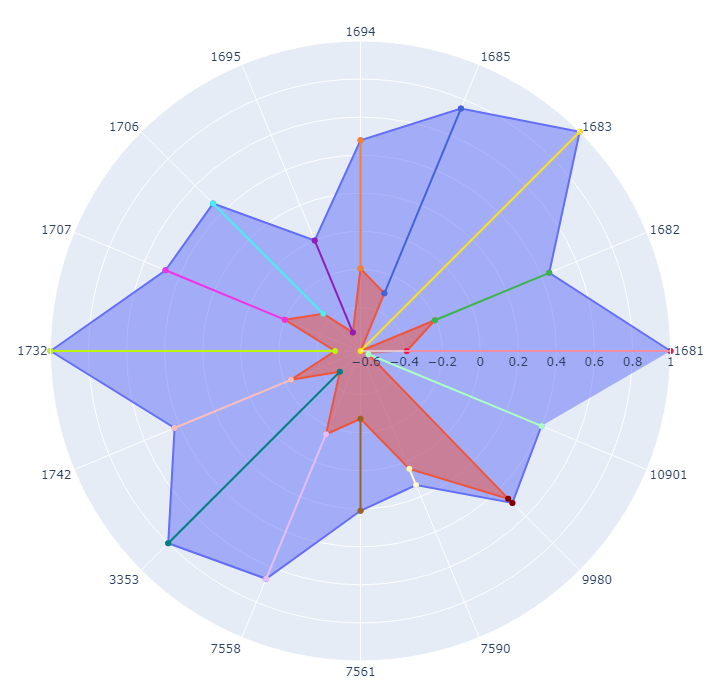
\includegraphics[width=0.7\textwidth]{images/social_barometer_public_health.png}
	\caption{Gráfico de Radar ilustrando a pressão social em relação ao tópico de Saúde Pública.}
	\label{fig:social_barometer_public_health}
\end{figure}

\begin{table}[htbp]
	\centering
	\caption{Métricas de pressão social do tópico de Saúde Pública}
	\label{tab:eventos_populares_public_health}
	\begin{tabular}{|l|c|c|c|c|}
		\hline
		\textbf{Tipo de Evento}                               & \textbf{Eventos} & \textbf{Score} & \textbf{Persona} \\
		\hline
		1707:Foco de mosquito da dengue/zika                  & 7                & -0.1986        & 0.4800           \\
		\hline
		1694:Descarte irregular de lixo                       & 6                & -0.1959        & 0.4783           \\
		\hline
		1685:Estabelecimento com acessibilidade irregular     & 5                & -0.3009        & 0.7500           \\
		\hline
		7590:Bueiro entupido                                  & 5                & 0.0413         & 0.1333           \\
		\hline
		1681:Ponto recorrente de poluição sonora              & 4                & -0.3863        & 1.0000           \\
		\hline
		1706:Infestação animais perigosos                     & 4                & -0.3524        & 0.4667           \\
		\hline
		1742:Vazamento de esgoto                              & 4                & -0.2332        & 0.4286           \\
		\hline
		3353:Aglomeração de pessoas                           & 4                & -0.4755        & 0.8000           \\
		\hline
		1682:Estabelecimento com condição sanitária irregular & 3                & -0.2063        & 0.4444           \\
		\hline
		7561:Ponto de alagamento                              & 3                & -0.2729        & 0.2105           \\
		\hline
		1683:Estabelecimento sem alvará                       & 2                & -0.6291        & 1.0000           \\
		\hline
		7558:Ocupação irregular de área pública               & 2                & -0.1556        & 0.6667           \\
		\hline
		9980:Atendimento na Clínica da Família                & 2                & 0.4684         & 0.5000           \\
		\hline
		10901:Esgoto a céu aberto                             & 2                & -0.5841        & 0.4000           \\
		\hline
		1695:Praia suja                                       & 1                & -0.5235        & 0.0000           \\
		\hline
		1732:Área com risco de deslizamento                   & 1                & -0.4953        & 1.0000           \\
		\hline
	\end{tabular}
\end{table}

Quando se observa o evento 'Atendimento na Clínica da Família', a análise revela um panorama mais otimista. Com um score médio de positiva e uma persona com tendencias a \textit{helper}, há uma inclinação mais positiva em relação ao serviço. Tal observação pode ser atribuída à satisfação com os serviços de saúde ofertados ou à qualidade do atendimento nestes estabelecimentos. Todavia, é essencial considerar que o número de postagens associado a esse evento é menor quando comparado a outros, o que pode influenciar na representatividade desta métrica.

Em contraste, eventos como 'Estabelecimento sem alvará' e 'Área com risco de deslizamento' denotaram uma postura altamente crítica por parte dos usuários, com personas máximas de \textit{complainer} e sentimentos negativos intensos. Esses resultados podem indicar uma grave preocupação dos cidadãos com a regularidade e segurança dos estabelecimentos e áreas urbanas, exigindo uma atenção imediata por parte dos gestores públicos.

Um aspecto intrigante se manifesta quando analisamos o evento 'Praia suja', que, embora tenha um sentimento negativo apresenta uma persona totalmente inclinada para o tipo \textit{helper}. Tal contradição sugere que, mesmo insatisfeitos com a condição das praias, os cidadãos estão dispostos a colaborar e ajudar na busca por soluções, demonstrando um senso de coletividade e responsabilidade ambiental.

No entanto, ao analisar eventos associados a doenças, como 'Foco de mosquito da dengue/zika', percebe-se uma preocupação evidente com uma pontuação de sentimento negativa, mas uma persona média mista. Esses valores indicam uma tendência moderada para o perfil \textit{complainer}, provavelmente reflexo da gravidade das consequências destas doenças e da necessidade urgente de ações de combate.

No que tange às palavras-chave extraídas, é possível identificar que termos como 'dengue' e 'médico' são proeminentes, com 425 e 68 ocorrências respectivamente. Esta predominância pode indicar uma ênfase na discussão sobre doenças endêmicas e na qualidade ou acessibilidade dos serviços médicos, constituindo-se como temas centrais nas discussões de zeladoria urbana relacionada à saúde.

A análise da pressão social em relação à saúde pública no Colab oferece um retrato profundo das percepções e inquietações dos cidadãos. Observamos que determinados eventos suscitam sentimentos predominantemente negativos, enquanto outros eventos revelam uma dicotomia mais equilibrada entre as atitudes de \textit{helper} e \textit{complainer}. Entender essas nuances é fundamental para que os responsáveis pela gestão pública possam se orientar de maneira mais eficaz, ajustando as intervenções e políticas de acordo com as reais demandas e sentimentos da comunidade. Esta abordagem não apenas realça a importância da participação cidadã na construção de cidades mais resilientes e inclusivas, mas também enfatiza o papel das plataformas digitais como ferramentas cruciais para capturar e analisar a voz da população em tempo real.

\subsection{Distanciamento Social}

Durante a pandemia de COVID-19, muitos usuários usaram o Colab para relatar problemas relacionados ao distanciamento social. Isso inclui aglomerações, o uso de máscaras e outras preocupações relacionadas à saúde pública. Essas discussões refletem a sensibilidade das comunidades à pandemia e a importância da conscientização sobre medidas de saúde.

\begin{figure}[htb]
	\centering
	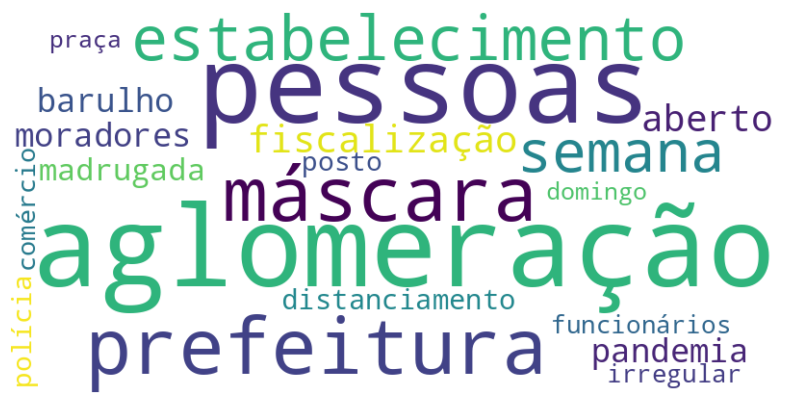
\includegraphics[width=0.7\textwidth]{images/wordcloud_social_distancing.png}
	\caption{Wordcloud com palavras mais frequentes em postagens sobre Distanciamento Social}
	\label{fig:wordcloud_social_distancing}
\end{figure}

Ao examinar os valores médios de score e personas para eventos relacionados ao distanciamento social, podemos observar uma série de tendências interessantes, onde diferentes eventos de zeladoria pública suscitam diversas reações por parte dos usuários da plataforma. Por exemplo, o evento 'Ônibus/trem/metrô superlotado', observamos que a persona média associada a esse evento é predominantemente de \textit{helper}. Isso indica que os usuários que se manifestam sobre a superlotação no transporte público têm uma atitude positiva e colaborativa em relação ao problema. Além disso, o score médio de sentimentos negativo sugere que, embora haja um reconhecimento das dificuldades enfrentadas, a maior parte das postagens possui um tom negativo, refletindo a insatisfação dos usuários com a situação.

No caso de 'Ônibus superlotado', tanto a persona média quanto o score médio de sentimentos atingem valores mais extremos. A persona média sugere que os usuários que comentam sobre ônibus superlotados são predominantemente do tipo \textit{complainer}, expressando críticas e insatisfação. O score médio de sentimentos negativo sugere uma forte reação negativa em relação à superlotação nos ônibus. Esses resultados demonstram uma alta pressão social em relação a esse problema específico, com uma clara predominância de opiniões críticas.

\begin{figure}[htb]
	\centering
	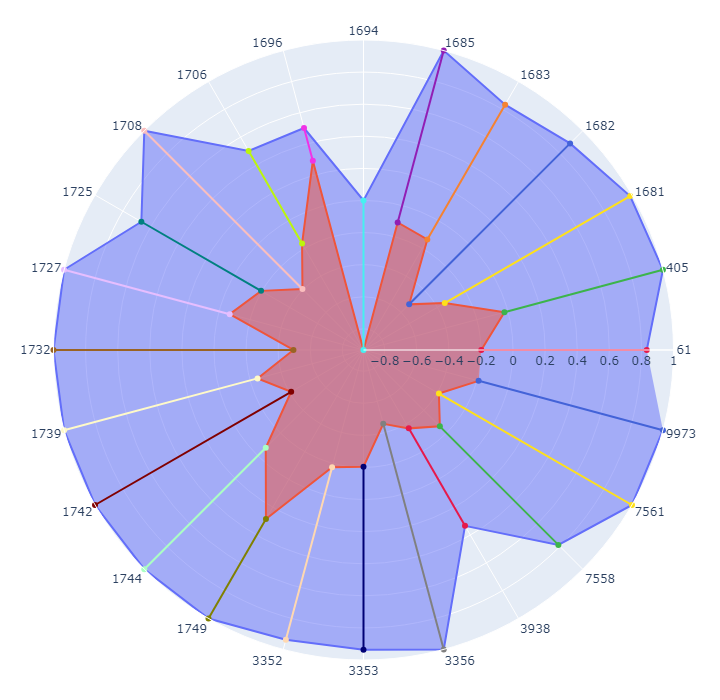
\includegraphics[width=0.7\textwidth]{images/social_barometer_social_distancing.png}
	\caption{Gráfico de Radar ilustrando a pressão social em relação ao tópico de Distanciamento Social.}
	\label{fig:social_barometer_social_distancing}
\end{figure}

\begin{table}[htbp]
	\centering
	\caption{Métricas de pressão social do tópico de Distanciamento Social}
	\label{tab:eventos_populares_social_distancing}
	\begin{tabular}{|l|c|c|c|c|}
		\hline
		\textbf{Tipo de Evento}                               & \textbf{Eventos} & \textbf{Score} & \textbf{Persona} \\
		\hline
		1681:Ponto recorrente de poluição sonora              & 4                & -0.3471        & 0.9867           \\
		\hline
		1682:Estabelecimento com condição sanitária irregular & 4                & -0.5293        & 0.8889           \\
		\hline
		7558:Ocupação irregular de área pública               & 4                & -0.2589        & 0.7857           \\
		\hline
		3353:Aglomeração de pessoas                           & 4                & -0.2041        & 0.9365           \\
		\hline
		3352:Comércio aberto irregularmente                   & 4                & -0.1758        & 0.9375           \\
		\hline
		1739:Evento Irregular                                 & 4                & -0.2484        & 1.0000           \\
		\hline
		61:Ônibus/trem/metrô superlotado                      & 3                & -0.1978        & 0.8333           \\
		\hline
		1749:Manutenção de semáforo                           & 3                & 0.2840         & 1.0000           \\
		\hline
		1683:Estabelecimento sem alvará                       & 3                & -0.1364        & 0.8333           \\
		\hline
		3938:Entulho na calçada/via pública                   & 3                & -0.3678        & 0.3333           \\
		\hline
		1706:Infestação animais perigosos                     & 3                & -0.1663        & 0.5000           \\
		\hline
		1725:Bloqueio na via                                  & 3                & -0.1948        & 0.6667           \\
		\hline
		405:Ônibus superlotado                                & 3                & -0.0226        & 1.0000           \\
		\hline
		7561:Ponto de alagamento                              & 2                & -0.3893        & 1.0000           \\
		\hline
		1732:Área com risco de deslizamento                   & 2                & -0.4953        & 1.0000           \\
		\hline
		1744:Ônibus danificado                                & 1                & -0.0703        & 1.0000           \\
		\hline
		1742:Vazamento de esgoto                              & 1                & -0.4113        & 1.0000           \\
		\hline
		1727:Equipamento público danificado                   & 1                & -0.0688        & 1.0000           \\
		\hline
		1708:Ponto de tráfico de drogas                       & 1                & -0.3938        & 1.0000           \\
		\hline
		3356:Ônibus fora do horário/rota                      & 1                & -0.4558        & 1.0000           \\
		\hline
	\end{tabular}
\end{table}

No contexto de 'Aglomeração de pessoas', a persona média indica que usuários que abordam esse tema tendem a assumir uma postura de \textit{helper}, demonstrando uma atitude positiva e colaborativa. No entanto, o score médio de sentimentos negativo sugere que, apesar da disposição para ajudar, ainda existe um sentimento negativo em relação à aglomeração de pessoas, possivelmente devido às implicações na propagação de doenças, como a COVID-19.

Ao explorar o evento 'Má conduta de motorista ou cobrador', observamos uma persona média quase exclusivamente do tipo \textit{complainer}, expressando críticas e insatisfação. O score médio de sentimentos reforça essa tendência negativa, destacando a forte pressão social relacionada ao comportamento inadequado de motoristas e cobradores de transporte público.

Por fim, o evento 'Estabelecimento com condição sanitária irregular' apresenta uma persona média sugerindo uma predominância de personas do tipo \textit{complainer}, com uma atitude crítica em relação à falta de conformidade com as normas sanitárias. O score médio de sentimentos reflete uma reação muito negativa por parte dos usuários, indicando uma preocupação séria e uma pressão social significativa relacionada a estabelecimentos que não seguem as diretrizes de saúde pública.

\subsection{Mudança Climática}

A análise da pressão social, especialmente no contexto das mudanças climáticas, é de grande relevância nos dias atuais. Os usuários do Colab demonstram uma crescente preocupação com os efeitos das mudanças climáticas, o que se torna evidente quando ocorrem chuvas intensas, tempestades e outros eventos climáticos adversos. Nesses momentos, os cidadãos recorrem à plataforma para documentar os impactos desses eventos na infraestrutura urbana, como danos a estradas, alagamentos, atrasos nos serviços de transporte público, riscos de deslizamento e muito mais. Essa tendência é particularmente significativa nas três cidades do sudeste do país que estão sob análise.

Além disso, os usuários também expressam preocupações relacionadas às altas temperaturas nos centros urbanos. Eles frequentemente compartilham suas insatisfações em relação à falta de preparo da infraestrutura pública para lidar com o calor, incluindo a escassez de ar-condicionado e ventilação adequada em espaços públicos, bem como a ausência de áreas verdes e arborização suficiente para proporcionar alívio em meio às altas temperaturas.

A complexidade dessas questões climáticas gera um debate polarizado entre os usuários do Colab. Por um lado, há aqueles que negam ou minimizam os efeitos das mudanças climáticas, questionando sua gravidade ou mesmo sua existência. Por outro lado, existem aqueles que advogam por políticas de mudança e ação climática, defendendo a necessidade de medidas concretas para mitigar os impactos ambientais e adaptar as cidades às mudanças climáticas. Essa polarização reflete-se nas postagens e discussões na plataforma, onde diferentes opiniões e perspectivas colidem.

Portanto, é fundamental explorar essa dinâmica de pressão social, uma vez que ela oferece insights valiosos sobre como os cidadãos das cidades do sudeste do Brasil percebem e reagem às questões climáticas. Essa análise não apenas revela a diversidade de opiniões e preocupações, mas também fornece informações valiosas para os tomadores de decisão e gestores públicos que buscam compreender as complexas dinâmicas urbanas relacionadas ao clima e desenvolver políticas eficazes para enfrentar esses desafios ambientais.

\begin{figure}[htb]
	\centering
	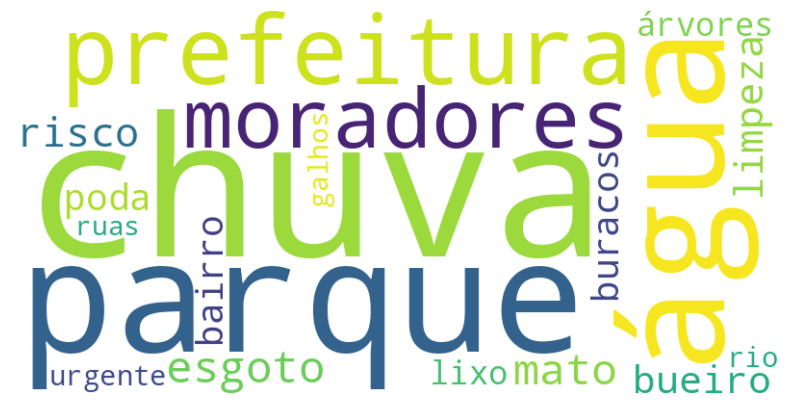
\includegraphics[width=0.7\textwidth]{images/wordcloud_weather.png}
	\caption{Wordcloud com palavras mais frequentes em postagens sobre Mudança Climática}
	\label{fig:wordcloud_weather}
\end{figure}

Ao observar os resultados, podemos notar que os eventos relacionados à mudança climática, como 'Praia suja' e 'Ponto de queimada irregular recorrente' apresentam personas predominantemente \textit{complainer}. Isso sugere que os usuários estão expressando preocupações e insatisfações em relação a esses problemas ambientais. Além disso, esses eventos também têm score médio negativo, o que indica que as postagens relacionadas a esses eventos tendem a conter sentimentos negativos.

Por outro lado, eventos como 'Limpeza de Canais' e 'Plantar uma árvore / Arborização' têm personas predominantemente \textit{helper}. Esses eventos também possuem score médio positivo, o que sugere que os usuários estão expressando atitudes colaborativas e positivas em relação a essas iniciativas. Isso indica um forte apoio da comunidade aos esforços de limpeza e arborização, o que reflete as sensibilidades da sociedade em relação às questões ambientais em tempos de mudança climática.

No entanto, vale destacar que eventos relacionados ao clima, como 'Calor nos centros urbanos' 'Falta de ar condicionado e ventilação adequada' e 'Chuva' apresentam resultados variados. Enquanto 'Calor nos centros urbanos' tem uma persona predominantemente \textit{complainer}, indicando insatisfação com o calor nas áreas urbanas, 'Chuva' apresenta uma persona mista e score médio ligeiramente negativo de, sugerindo uma mistura de opiniões sobre as chuvas e eventos climáticos relacionados.

É interessante notar que os eventos relacionados à mudança climática podem evocar respostas polarizadas da comunidade. Alguns eventos, como a limpeza de canais e a arborização, são amplamente apoiados, refletindo uma disposição da comunidade para tomar medidas positivas para enfrentar a mudança climática. Por outro lado, eventos que evidenciam problemas, como praias sujas e queimadas irregulares, provocam insatisfações e críticas.

Essa análise sugere que os usuários do Colab estão cientes dos desafios relacionados à mudança climática e estão dispostos a apoiar ações positivas, mas também expressam descontentamento quando confrontados com problemas ambientais. A polarização de opiniões em relação a eventos climáticos pode indicar a complexidade dessas questões e a necessidade de estratégias de engajamento e comunicação mais eficazes para lidar com as preocupações dos cidadãos.

\begin{figure}[htb]
	\centering
	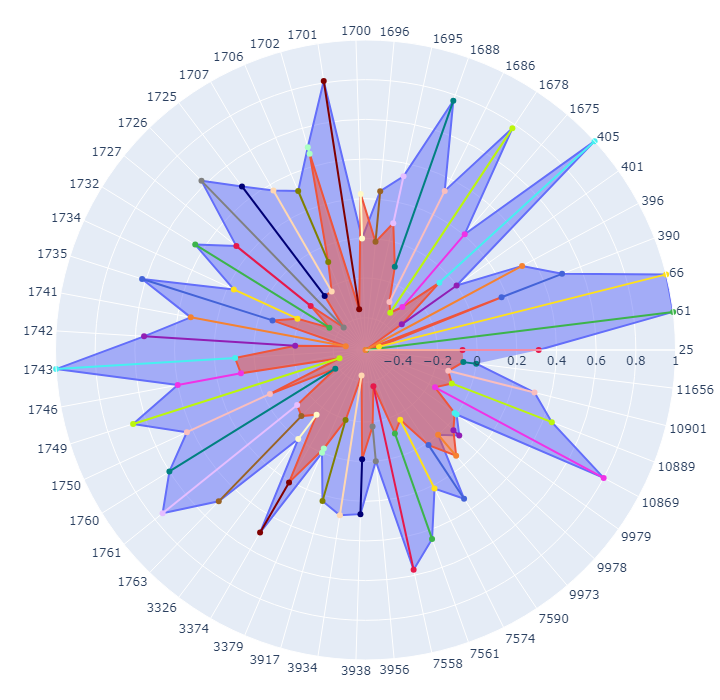
\includegraphics[width=0.7\textwidth]{images/social_barometer_weather.png}
	\caption{Gráfico de Radar ilustrando a pressão social em relação ao tópico de Mudança Climática.}
	\label{fig:social_barometer_weather}
\end{figure}

\begin{table}[htbp]
	\centering
	\caption{Métricas de pressão social do tópico de Mudança Climática}
	\label{tab:eventos_populares_weather}
	\begin{tabular}{|l|c|c|c|c|}
		\hline
		\textbf{Tipo de Evento}                         & \textbf{Eventos} & \textbf{Score} & \textbf{Persona} \\
		\hline
		7574:Poda de árvore                             & 13               & -0.1698        & 0.2177           \\
		\hline
		1734:Retirada de árvore                         & 10               & -0.1851        & 0.1681           \\
		\hline
		1727:Equipamento público danificado             & 9                & -0.2080        & 0.2727           \\
		\hline
		3938:Entulho na calçada/via pública             & 8                & -0.0117        & 0.2651           \\
		\hline
		3934:Fiação irregular                           & 7                & -0.4324        & 0.2800           \\
		\hline
		1696:Mato alto                                  & 7                & -0.0151        & 0.2411           \\
		\hline
		25:Vazamento de água                            & 6                & -0.0735        & 0.3103           \\
		\hline
		7590:Bueiro entupido                            & 6                & 0.0125         & 0.3368           \\
		\hline
		3917:Calçada irregular                          & 6                & -0.1955        & 0.2292           \\
		\hline
		1701:Desmatamento irregular                     & 6                & -0.3553        & 0.8095           \\
		\hline
		1707:Foco de mosquito da dengue/zika            & 5                & -0.2218        & 0.3659           \\
		\hline
		10889:Placa de sinalização quebrada/inexistente & 5                & -0.0963        & 0.4444           \\
		\hline
		10869:Ônibus/trem/metrô danificado              & 5                & -0.1651        & 0.8000           \\
		\hline
		7561:Ponto de alagamento                        & 5                & -0.1167        & 0.4471           \\
		\hline
		7558:Ocupação irregular de área pública         & 5                & -0.3763        & 0.5714           \\
		\hline
		1732:Área com risco de deslizamento             & 5                & -0.3487        & 0.4468           \\
		\hline
		1742:Vazamento de esgoto                        & 5                & -0.2076        & 0.5556           \\
		\hline
		1706:Infestação animais perigosos               & 5                & -0.0807        & 0.3077           \\
		\hline
		11656:Plantar uma árvore / Arborização          & 5                & -0.0657        & 0.0000           \\
		\hline
		1678:Falta de água                              & 4                & -0.3369        & 0.7778           \\
		\hline
	\end{tabular}
\end{table}

A análise da pressão social, especialmente no contexto das mudanças climáticas, revela uma série de perspectivas e preocupações dos usuários do Colab nas cidades de Niterói, Santo André e Mesquita. Os resultados apontam para uma crescente conscientização sobre os efeitos das mudanças climáticas, com eventos climáticos adversos, como chuvas intensas e tempestades, provocando uma resposta significativa por parte da comunidade. Esses eventos são documentados de forma abrangente, com os cidadãos destacando os impactos na infraestrutura urbana, incluindo danos a estradas, alagamentos, atrasos nos serviços de transporte público e riscos de deslizamento. Além disso, a preocupação com as altas temperaturas nos centros urbanos é evidente nas postagens dos usuários. Eles frequentemente manifestam insatisfação em relação à falta de preparo da infraestrutura pública para lidar com o calor, enfatizando a necessidade de mais ar-condicionado, ventilação adequada, áreas verdes e arborização. A análise também revela uma divisão de opiniões e polarização em relação às questões climáticas. Por um lado, há aqueles que negam ou minimizam os efeitos das mudanças climáticas, questionando sua gravidade. Por outro lado, existem defensores de políticas de mudança climática que advogam por medidas concretas para mitigar os impactos ambientais e adaptar as cidades às mudanças climáticas.

Os eventos relacionados à mudança climática variam em termos de pressão social, com alguns, como a limpeza de canais e a arborização, recebendo forte apoio e refletindo personas predominantemente \textit{helper} e sentimentos positivos. No entanto, eventos que evidenciam problemas ambientais, como praias sujas e queimadas irregulares, geram insatisfações e críticas, refletindo personas predominantemente \textit{complainer} e sentimentos negativos. Esses resultados destacam a complexidade das questões climáticas e a necessidade de abordagens holísticas e estratégias de engajamento eficazes para enfrentar os desafios da mudança climática em nível local. A compreensão dessas dinâmicas de pressão social é fundamental para orientar políticas e ações que respondam às preocupações dos cidadãos e promovam um ambiente urbano mais sustentável e resiliente diante das mudanças climáticas. Em última análise, a análise da pressão social oferece insights valiosos para tomadores de decisão e gestores públicos que buscam criar soluções eficazes para enfrentar os impactos das mudanças climáticas em suas comunidades.

\subsection{Paisagismo}

A paisagem urbana desempenha um papel crucial na qualidade de vida dos cidadãos e no bem-estar das comunidades locais. A gestão adequada das áreas verdes, árvores, parques e espaços públicos não apenas contribui para a estética das cidades, mas também desempenha um papel essencial na mitigação das mudanças climáticas, na promoção da saúde pública e no fomento de uma sensação de pertencimento à comunidade. É nesse contexto que o tópico de 'paisagismo' se revela como uma questão de pressão social hiperlocal relevante e de grande interesse.

O paisagismo urbano não se limita apenas à beleza visual das cidades; ele abrange aspectos como o plantio e a manutenção de árvores, a criação de áreas verdes, a poda de vegetação, entre outros. Essas práticas têm implicações diretas na qualidade do ar, na regulação da temperatura local, na absorção de poluentes e na promoção da biodiversidade urbana. Além disso, o paisagismo influencia a vida cotidiana dos habitantes urbanos, afetando o acesso a sombras em áreas públicas, a oferta de espaços para atividades ao ar livre e o senso de identidade e pertencimento à cidade.

\begin{figure}[htb]
	\centering
	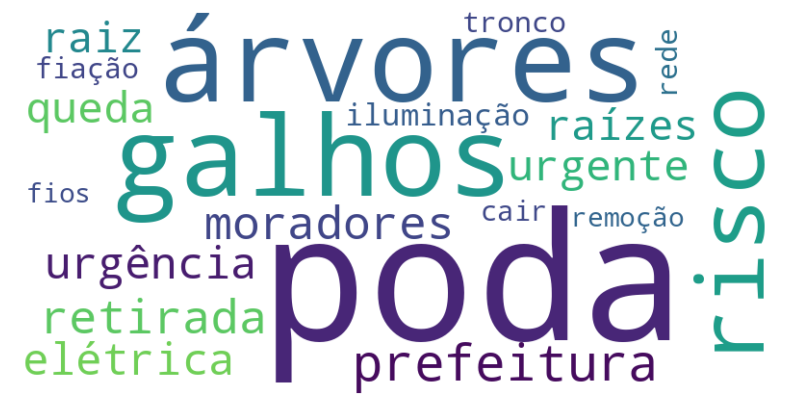
\includegraphics[width=0.7\textwidth]{images/wordcloud_landscape.png}
	\caption{Wordcloud com palavras mais frequentes em postagens sobre Paisagismo}
	\label{fig:wordcloud_landscape}
\end{figure}

A relevância do paisagismo como um tópico de pressão social hiperlocal se manifesta na maneira como os cidadãos interagem com a sua paisagem urbana e como expressam suas opiniões e preocupações relacionadas a esse tema. Através de plataformas de participação cidadã, como o Colab, os residentes urbanos têm a oportunidade de compartilhar suas perspectivas, denunciar problemas e influenciar diretamente as decisões relacionadas à gestão do paisagismo em suas comunidades. A compreensão dessas dinâmicas é fundamental para gestores públicos, urbanistas e tomadores de decisão, pois ajuda a orientar políticas e práticas que melhor atendam às necessidades e desejos das comunidades locais.

\begin{figure}[htb]
	\centering
	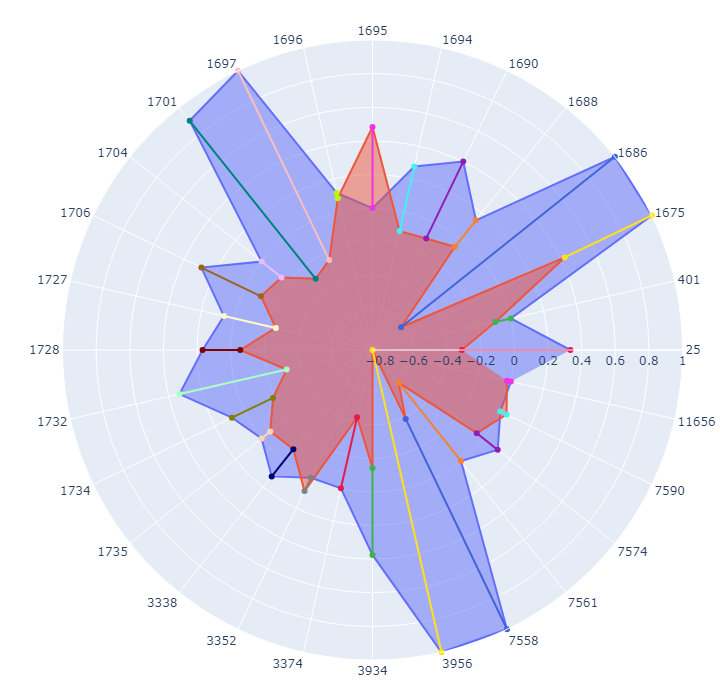
\includegraphics[width=0.7\textwidth]{images/social_barometer_landscape.png}
	\caption{Gráfico de Radar ilustrando a pressão social em relação ao tópico de Paisagismo}
	\label{fig:social_barometer_landscape}
\end{figure}

\begin{table}[htbp]
	\centering
	\caption{Métricas de pressão social do tópico de Paisagismo}
	\label{tab:eventos_populares_landscape}
	\begin{tabular}{|l|c|c|c|c|}
		\hline
		\textbf{Tipo de Evento}                 & \textbf{Eventos} & \textbf{Score} & \textbf{Persona} \\
		\hline
		7574:Poda de árvore                     & 10               & -0.0504        & 0.1086           \\
		\hline
		1734:Retirada de árvore                 & 9                & -0.1876        & 0.0840           \\
		\hline
		1696:Mato alto                          & 7                & 0.0825         & 0.1143           \\
		\hline
		7590:Bueiro entupido                    & 6                & 0.0411         & 0.0000           \\
		\hline
		1701:Desmatamento irregular             & 6                & -0.3021        & 0.9000           \\
		\hline
		1727:Equipamento público danificado     & 6                & -0.2540        & 0.0625           \\
		\hline
		11656:Plantar uma árvore / Arborização  & 5                & -0.0235        & 0.0000           \\
		\hline
		1694:Descarte irregular de lixo         & 5                & -0.1186        & 0.2759           \\
		\hline
		1732:Área com risco de deslizamento     & 5                & -0.3202        & 0.3333           \\
		\hline
		1706:Infestação animais perigosos       & 4                & -0.1076        & 0.2857           \\
		\hline
		7558:Ocupação irregular de área pública & 4                & -0.3889        & 1.0000           \\
		\hline
		3934:Fiação irregular                   & 4                & -0.1428        & 0.3750           \\
		\hline
		25:Vazamento de água                    & 4                & -0.3128        & 0.3333           \\
		\hline
		1695:Praia suja                         & 4                & 0.4822         & 0.0000           \\
		\hline
		1704:Calçada inexistente                & 3                & -0.1514        & 0.0000           \\
		\hline
		3338:Iluminação pública irregular       & 3                & -0.0891        & 0.1176           \\
		\hline
		3352:Comércio aberto irregularmente     & 3                & 0.0877         & 0.0000           \\
		\hline
		1690:Lâmpada acesa de dia               & 3                & -0.1075        & 0.4000           \\
		\hline
		1688:Falta de energia                   & 3                & -0.0585        & 0.1429           \\
		\hline
		7561:Ponto de alagamento                & 3                & -0.5951        & 0.0000           \\
		\hline
	\end{tabular}
\end{table}

Ao analisar os dados de pressão social hiperlocal relacionados ao paisagismo, entendemos como os cidadãos percebem e reagem às intervenções e práticas de paisagismo em suas cidades. É interessante observar que alguns tipos de eventos de paisagismo apresentam uma persona predominantemente \textit{helper}, caracterizada por atitudes positivas e colaborativas em relação aos eventos. Um exemplo notável é o evento 'Plantar uma árvore / Arborização', que possui uma persona média próxima de 0 e um score médio de sentimento negativo próximo de 0. Isso sugere que os usuários tendem a expressar apoio e entusiasmo em relação à arborização urbana, refletindo uma atitude favorável em relação a iniciativas de paisagismo que envolvem o plantio de árvores.

Por outro lado, alguns eventos de paisagismo apresentam personas predominantemente \textit{complainer}, indicando uma postura mais crítica e insatisfeita por parte dos usuários. Por exemplo, o evento 'Falta de energia' tem uma persona média de aproximadamente 0.14 e um score médio de sentimento negativo próximo de -0.06. Embora a persona média não seja muito alta, o score médio negativo sugere que os usuários tendem a expressar insatisfação em relação à falta de energia em contextos de paisagismo urbano. Isso pode indicar que os cidadãos esperam uma infraestrutura mais confiável e eficaz em relação à energia elétrica em espaços públicos.

Além disso, outros eventos de paisagismo, como 'Calçada inexistente' e 'Faixa de pedestre apagada' também apresentam personas predominantemente \textit{complainer}. A falta de calçadas e faixas de pedestres em boas condições pode ser uma preocupação significativa para os usuários, refletindo-se em personas médias de aproximadamente 0 e scores médios negativos. Isso sugere que os usuários estão insatisfeitos com a falta de infraestrutura básica para pedestres nas áreas urbanas, o que pode afetar diretamente a acessibilidade e segurança. Eventos como 'Praia suja' também apresentam personas predominantemente \textit{complainer} e scores médios de sentimento positivo de aproximadamente 0.48. Isso indica que, embora os usuários expressem preocupação com a sujeira nas praias, eles também podem estar dispostos a apoiar iniciativas de limpeza e conservação, refletindo uma atitude crítica, mas com espaço para ação positiva.

Outro evento de destaque é a 'Poda de árvore' que apresenta uma persona média de aproximadamente 0.11 e um score médio de sentimento positivo de cerca de 0.04. Esses dados apontam para a complexidade da questão, uma vez que revelam que os usuários do Colab têm opiniões divergentes sobre a poda de árvores. Ao analisar manualmente algumas postagens desse grupo de eventos, podemos contestar que, alguns usuários podem apoiar a poda como uma medida necessária para manter a segurança e a estética das áreas urbanas, outros expressam preocupações relacionadas à preservação das áreas verdes da cidade, ao impacto na sombra proporcionada pelas árvores e às implicações das mudanças climáticas. Essa polarização de opiniões em torno do evento de poda de árvores indica que o tópico de paisagismo no Colab é uma fonte de debates e discussões significativas, refletindo as diversas perspectivas e preocupações dos usuários em relação às práticas de manejo da vegetação urbana.

Eventos como 'Plantar uma árvore / Arborização' recebem um forte apoio, refletindo uma disposição da comunidade para adotar uma postura colaborativa e positiva em relação à arborização urbana. No entanto, outros eventos, como 'Falta de energia' 'Calçada inexistente' e 'Faixa de pedestre apagada' geram insatisfações e críticas, indicando a necessidade de melhorias na infraestrutura urbana relacionada ao paisagismo. Eventos como 'Praia suja' e 'Poda de árvore' apresentam uma mistura de opiniões, com uma persona predominantemente \textit{complainer} mas espaço para ações positivas.

Os resultados sugerem que os usuários do Colab têm uma compreensão variada das questões de paisagismo urbano e que suas opiniões podem ser influenciadas por fatores contextuais, como a natureza específica do evento. A polarização de opiniões em relação a eventos de paisagismo pode indicar a complexidade dessas questões e a necessidade de estratégias de engajamento e comunicação mais eficazes para lidar com as preocupações dos cidadãos. No entanto, em geral, a análise da pressão social destaca a importância de considerar as opiniões da comunidade ao planejar e implementar iniciativas de paisagismo urbano, buscando atender às expectativas e necessidades dos cidadãos.

\subsection{Meio Ambiente}

O tópico de meio ambiente é de extrema importância e relevância para as comunidades urbanas em todo o mundo. As questões ambientais têm um impacto direto na qualidade de vida dos cidadãos nas cidades, afetando aspectos como a saúde pública, o acesso a espaços verdes, a qualidade do ar e da água, a biodiversidade urbana e até mesmo o clima local. A qualidade do ambiente urbano influencia a saúde física e mental dos habitantes das cidades. Questões como poluição do ar, contaminação da água, falta de áreas verdes e exposição a substâncias tóxicas podem contribuir para problemas de saúde, como doenças respiratórias, alergias, problemas cardiovasculares e estresse. Além disso, a degradação ambiental pode ter impactos socioeconômicos, como desvalorização imobiliária e deslocamento de comunidades de baixa renda de áreas afetadas pela degradação ambiental. A disponibilidade de espaços verdes, como parques e praças, é essencial para a qualidade de vida nas cidades, proporcionando locais de recreação, contato com a natureza e promoção da saúde física e mental. Além disso, a preservação de árvores e áreas verdes urbanas desempenha um papel importante na regulação do clima local, na redução do calor urbano e na melhoria da qualidade do ar. A questão ambiental também está intrinsecamente ligada à sustentabilidade das cidades no longo prazo. O crescimento urbano desordenado, a poluição e o desperdício de recursos naturais podem comprometer a capacidade das cidades de atender às necessidades das gerações futuras. Portanto, a promoção de práticas sustentáveis, como reciclagem, redução do consumo de energia e transporte público eficiente, é essencial para garantir um ambiente urbano saudável e habitável no futuro.

A crescente necessidade de entender e decodificar a opinião pública em relação a questões ambientais não é apenas vital para os formuladores de políticas, mas também para compreender o cenário sócio-político de uma região. Baseando-se nas métricas de pressão social disponibilizadas, é possível delinear diversas conclusões significativas sobre a opinião das pessoas em relação a temas ambientais.

\begin{figure}[htb]
	\centering
	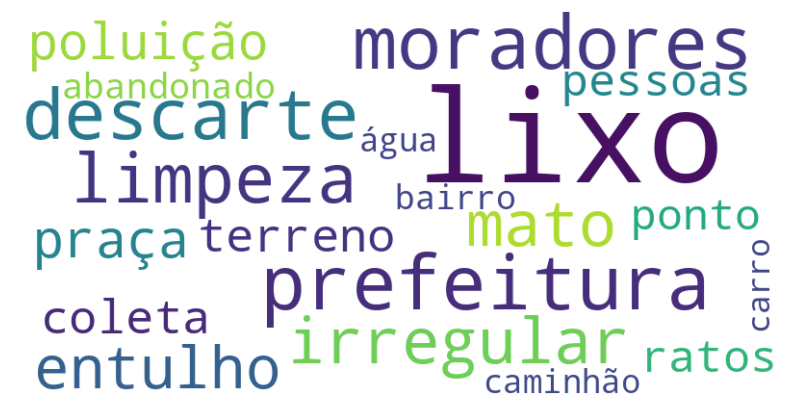
\includegraphics[width=0.7\textwidth]{images/wordcloud_environment.png}
	\caption{Wordcloud com palavras mais frequentes em postagens sobre Meio Ambiente}
	\label{fig:wordcloud_environment}
\end{figure}

Ao analisar a persona média atribuída aos usuários que participam das discussões sobre o meio ambiente no Colab, observamos uma interessante polarização nas opiniões e atitudes dos participantes. Em alguns eventos, como 'Caça ilegal' e 'Conservação (via pública)', a persona predominante é a \textit{helper}, o que sugere que os usuários que se envolvem nesses tópicos tendem a adotar uma abordagem colaborativa e positiva. Essa persona reflete um desejo de contribuir para soluções construtivas e uma forte preocupação com questões ambientais.

No entanto, em eventos como 'Coleta de container' e 'Falta de energia', observamos uma predominância da persona \textit{helper}. Isso indica que os usuários que comentam nesses eventos estão inclinados a expressar insatisfação e críticas em relação a problemas específicos, como a coleta de lixo inadequada ou interrupções no fornecimento de energia elétrica. Essa persona reflete uma frustração considerável entre os usuários em relação à qualidade dos serviços públicos relacionados a esses eventos.

\begin{figure}[htb]
	\centering
	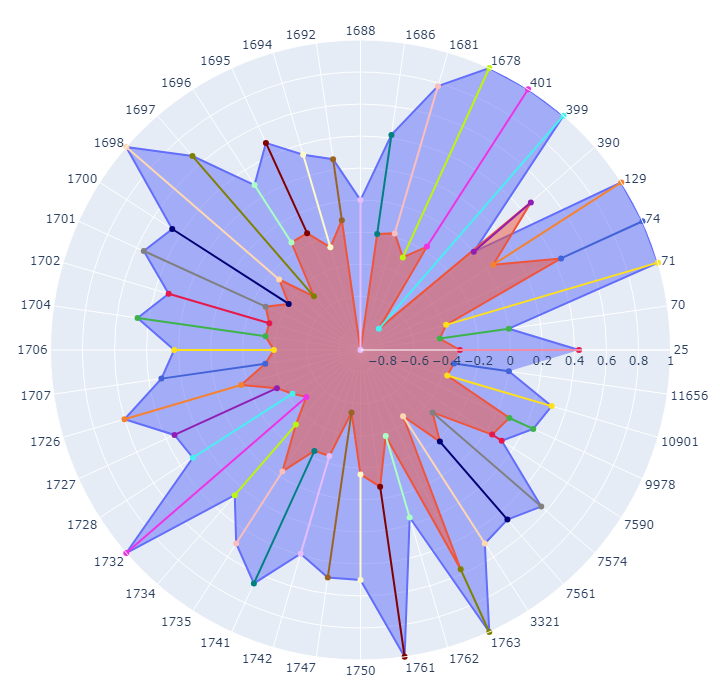
\includegraphics[width=0.7\textwidth]{images/social_barometer_environment.png}
	\caption{Gráfico de Radar ilustrando a pressão social em relação ao tópico de Meio Ambiente}
	\label{fig:social_barometer_environment}
\end{figure}

\begin{table}[htbp]
	\centering
	\caption{Métricas de pressão social do tópico de Meio Ambiente}
	\label{tab:eventos_populares_environment}
	\begin{tabular}{|l|c|c|c|c|}
		\hline
		\textbf{Tipo de Evento}                     & \textbf{Eventos} & \textbf{Score} & \textbf{Persona} \\
		\hline
		1694:Descarte irregular de lixo             & 9                & -0.2679        & 0.3349           \\
		\hline
		1701:Desmatamento irregular                 & 8                & -0.2849        & 0.5517           \\
		\hline
		7574:Poda de árvore                         & 8                & -0.3409        & 0.5574           \\
		\hline
		1700:Ponto de queimada irregular recorrente & 8                & -0.4036        & 0.4615           \\
		\hline
		1742:Vazamento de esgoto                    & 7                & -0.2459        & 0.3902           \\
		\hline
		1696:Mato alto                              & 7                & -0.1383        & 0.2885           \\
		\hline
		1728:Imóvel ou terreno abandonado           & 6                & -0.4314        & 0.3084           \\
		\hline
		7590:Bueiro entupido                        & 6                & 0.0412         & 0.1121           \\
		\hline
		1681:Ponto recorrente de poluição sonora    & 6                & -0.1772        & 0.7814           \\
		\hline
		1697:Maus tratos a animais                  & 5                & -0.4923        & 0.6667           \\
		\hline
		25:Vazamento de água                        & 5                & -0.3153        & 0.4286           \\
		\hline
		1686:Emissão de fumaça preta                & 5                & -0.2038        & 0.4211           \\
		\hline
		1704:Calçada inexistente                    & 4                & -0.3371        & 0.4706           \\
		\hline
		1727:Equipamento público danificado         & 4                & -0.3624        & 0.3409           \\
		\hline
		1695:Praia suja                             & 4                & -0.1338        & 0.4857           \\
		\hline
		1734:Retirada de árvore                     & 4                & -0.3201        & 0.2632           \\
		\hline
		1732:Área com risco de deslizamento         & 3                & -0.4890        & 1.0000           \\
		\hline
		1741:Manutenção de ciclovia/ciclofaixa      & 3                & -0.2437        & 0.6667           \\
		\hline
		1707:Foco de mosquito da dengue/zika        & 3                & -0.3356        & 0.3200           \\
		\hline
		7561:Ponto de alagamento                    & 3                & -0.1793        & 0.4651           \\
		\hline
	\end{tabular}
\end{table}

No que diz respeito às métricas de pressão social, primeiramente, é importante destacar que os eventos relacionados à proteção dos animais, como 'Caça ilegal' e 'Maus tratos a animais' têm uma persona média predominantemente \textit{helper}. Isso indica que os usuários que participam dessas discussões tendem a adotar uma abordagem colaborativa e positiva quando se trata de proteger a fauna. Essa persona \textit{helper} sugere que eles estão dispostos a contribuir para a preservação da vida selvagem e estão preocupados com o bem-estar dos animais. Podemos inferir que esses usuários provavelmente experimentam sentimentos de empatia, responsabilidade ambiental e um desejo genuíno de fazer a diferença positiva em relação à fauna.

Por outro lado, eventos relacionados a problemas de saneamento básico e conservação da água, como 'Coleta de container' e 'Esgoto a céu aberto' atraem uma persona média predominantemente \textit{complainer}. Isso sugere que os usuários que participam dessas discussões estão mais propensos a expressar insatisfação e críticas em relação a questões específicas, como problemas na coleta de lixo e esgoto a céu aberto. Essa persona mais inclinada a criticar pode indicar que esses usuários estão experimentando sentimentos de frustração, descontentamento e desconfiança em relação aos serviços de saneamento básico relacionados a esses eventos. Eles podem perceber esses problemas como falhas no sistema e podem estar em busca de melhorias.

A análise dos eventos de paisagismo e arborização revela uma persona média predominantemente \textit{helper} em eventos como 'Plantar uma árvore / Arborização'. Isso sugere que os usuários que participam dessas discussões estão dispostos a contribuir para a melhoria das áreas verdes urbanas e para a arborização da cidade. Eles provavelmente experimentam sentimentos de apoio a iniciativas de paisagismo e reconhecem a importância de áreas verdes para a qualidade de vida na cidade. Esses usuários podem ser motivados por sentimentos de bem-estar, amor pela natureza e desejo de tornar o ambiente urbano mais saudável. No que diz respeito aos alagamentos, eventos como 'Ponto de alagamento' recebem uma persona média predominantemente \textit{complainer}. Isso indica que os usuários que participam dessas discussões estão insatisfeitos com problemas de alagamento na cidade e estão mais inclinados a expressar críticas. Essa persona sugere que esses usuários podem estar experimentando sentimentos de frustração, desconforto e preocupação com os impactos dos alagamentos em suas vidas e comunidades.

As métricas de persona média e score médio também refletem a polarização nas discussões sobre mudanças climáticas. Eventos como 'Ponto de queimada irregular recorrente' e 'Desmatamento irregular' atraem uma persona média predominantemente \textit{complainer}. Isso indica que os usuários que participam dessas discussões estão mais propensos a expressar descontentamento e críticas em relação a práticas prejudiciais ao meio ambiente, como incêndios florestais e desmatamento ilegal. Essa persona mais inclinada a criticar sugere que esses usuários podem estar experimentando sentimentos de preocupação, indignação e urgência em relação às mudanças climáticas e à degradação ambiental.

Em relação à popularidade dos eventos, é notável que eventos como 'Descarte irregular de lixo' e 'Poda de árvore' recebam uma quantidade significativa de postagens. Isso pode ser interpretado como um indicativo de que os usuários estão ativamente envolvidos em discussões sobre questões relacionadas ao saneamento básico e à manutenção de áreas verdes urbanas. Essa popularidade pode estar relacionada ao fato de que esses eventos são altamente relevantes para a qualidade de vida nas cidades e, como resultado, os usuários estão dispostos a compartilhar suas opiniões e experiências sobre esses tópicos.

No geral, a análise detalhada das métricas de pressão social relacionadas ao meio ambiente destaca a diversidade de opiniões e sentimentos dos usuários do Colab em relação a questões ambientais. Essas métricas indicam que os usuários têm uma ampla gama de preocupações e perspectivas quando se trata de proteger a fauna, abordar questões de saneamento básico, promover o paisagismo urbano, lidar com as mudanças climáticas e enfrentar problemas de alagamento. Essa análise também revela áreas de insatisfação que precisam ser abordadas para melhorar a qualidade dos serviços e iniciativas relacionados ao meio ambiente. Em última análise, a compreensão dessas métricas de pressão social auxilia na promoção de discussões construtivas e na tomada de decisões informadas em relação a questões ambientais nas comunidades urbanas.

\subsection{Gentrificação}

A gentrificação tem se consolidado como um dos tópicos mais debatidos nas discussões sobre desenvolvimento urbano, desencadeando paixões e preocupações de diferentes partes da população. Dada a sua natureza multidimensional, é imperativo entender as nuances de como a gentrificação é percebida e quais as principais áreas de preocupação. Através da análise de dados de postagens de eventos de zeladoria pública no Colab, tentaremos destrinchar as diversas facetas desse fenômeno.

Os dados revelam, por exemplo, uma certa polaridade nas postagens. Há evidências de que alguns usuários, provavelmente proprietários de imóveis ou com algum interesse econômico na área, reportam eventos principalmente nas zonas onde possuem propriedades. O fato de reportarem focos como 'desvalorização da área imobiliária' sugere uma preocupação com a deterioração e possível depreciação de seus investimentos. Por outro lado, a presença de palavras-chave como 'despejo' e 'favelização' indica uma preocupação de outros usuários com os efeitos adversos da gentrificação, particularmente a expulsão de moradores de longa data e a falta de acesso a espaços públicos.

\begin{figure}[htb]
	\centering
	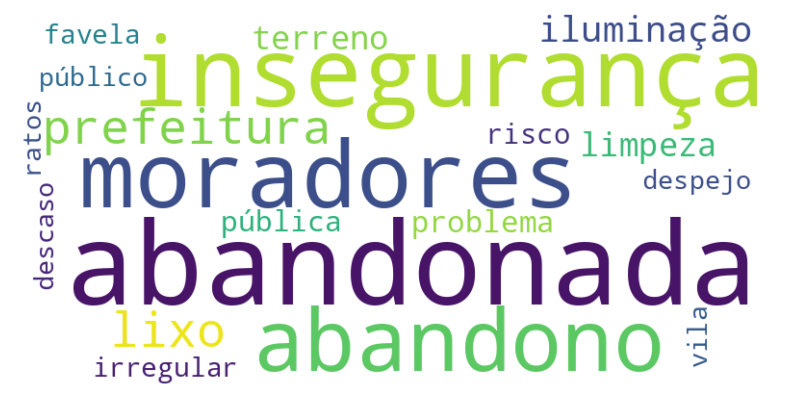
\includegraphics[width=0.7\textwidth]{images/wordcloud_gentrification.png}
	\caption{Wordcloud com palavras mais frequentes em postagens sobre Gentrificação}
	\label{fig:wordcloud_gentrification}
\end{figure}

Sob a perspectiva do score de sentimentos, por exemplo, 'Ponto recorrente de poluição sonora' tem um score médio de -0.487, indicando um sentimento predominantemente negativo. Esse sentimento negativo é também evidenciado em eventos como 'Desmatamento irregular', com um score de -0.292, e 'Esgoto a céu aberto', com um score ainda mais baixo de -0.815. Tais sentimentos sugerem uma percepção de negligência e abandono em determinadas áreas. Por outro lado, o evento 'Parque/praça' tem um score positivo de 0.5699, indicando uma opinião positiva ou talvez uma aspiração da comunidade por espaços públicos bem conservados. O valor da persona média para muitos dos eventos se inclina fortemente para 1.0. sugerindo que existe uma persona predominante que pode ser identificada como \textit{complainer} em muitos dos tópicos. Isso pode ser interpretado como uma evidência de que há uma forte expressão de insatisfação e demanda por melhores condições e serviços. Eventos como 'Ponto recorrente de exploração sexual de menores' e 'Área com risco de deslizamento', ambos com scores negativos e persona média inclinada para 1.0. ressaltam a gravidade das questões em jogo. A presença de tais eventos indica a necessidade urgente de intervenções e uma possível insatisfação com a inação das autoridades. Quando comparamos eventos populares - aqueles com maior contagem de eventos, como 'Descarte irregular de lixo' e 'Imóvel ou terreno abandonado', percebemos que a preocupação com a degradação e a falta de zeladoria são temas recorrentes. A frequência dessas postagens sugere que, para muitos usuários, a gentrificação não é apenas sobre a chegada de novos moradores ou estabelecimentos, mas também sobre a negligência e o abandono de áreas que anteriormente eram consideradas valiosas.

\begin{figure}[htb]
	\centering
	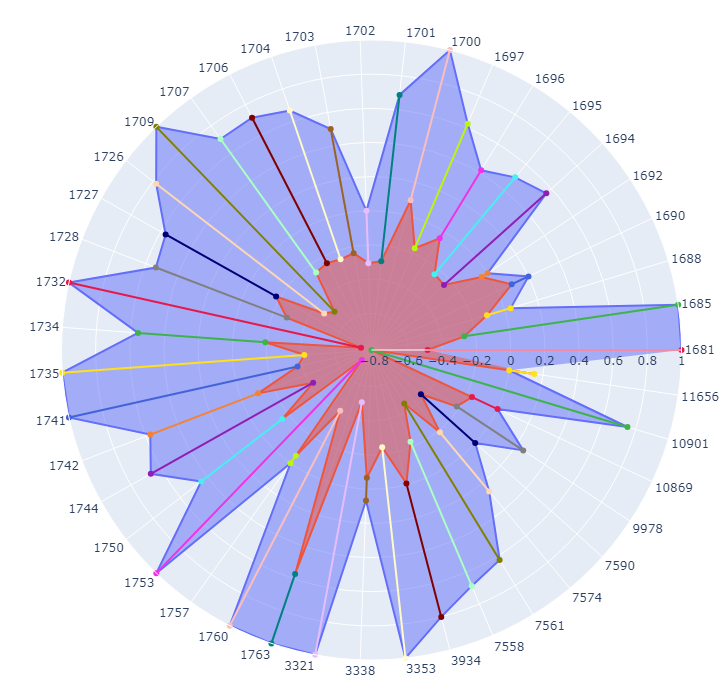
\includegraphics[width=0.7\textwidth]{images/social_barometer_gentrification.png}
	\caption{Gráfico de Radar ilustrando a pressão social em relação ao tópico de Gentrificação}
	\label{fig:social_barometer_gentrification}
\end{figure}

\begin{table}[htbp]
	\centering
	\caption{Métricas de pressão social do tópico de Gentrificação}
	\label{tab:eventos_populares_social_gentrification}
	\begin{tabular}{|l|c|c|c|c|}
		\hline
		\textbf{Tipo de Evento}                  & \textbf{Eventos} & \textbf{Score} & \textbf{Persona} \\
		\hline
		1694:Descarte irregular de lixo          & 11               & -0.2451        & 0.5593           \\
		\hline
		7558:Ocupação irregular de área pública  & 11               & -0.2313        & 0.6857           \\
		\hline
		1728:Imóvel ou terreno abandonado        & 11               & -0.2842        & 0.5366           \\
		\hline
		1681:Ponto recorrente de poluição sonora & 9                & -0.4871        & 1.0000           \\
		\hline
		1696:Mato alto                           & 8                & -0.0485        & 0.4173           \\
		\hline
		1727:Equipamento público danificado      & 7                & -0.1749        & 0.5672           \\
		\hline
		1742:Vazamento de esgoto                 & 6                & -0.1044        & 0.5714           \\
		\hline
		1701:Desmatamento irregular              & 5                & -0.2925        & 0.6875           \\
		\hline
		1726:Patrimônio histórico em risco       & 4                & -0.4648        & 0.7778           \\
		\hline
		10901:Esgoto a céu aberto                & 4                & -0.8154        & 0.7500           \\
		\hline
		7574:Poda de árvore                      & 4                & -0.1893        & 0.2619           \\
		\hline
		7561:Ponto de alagamento                 & 4                & -0.4481        & 0.6250           \\
		\hline
		3353:Aglomeração de pessoas              & 4                & -0.2428        & 1.0000           \\
		\hline
		1750:Varrição                            & 4                & -0.1550        & 0.4444           \\
		\hline
		1734:Retirada de árvore                  & 4                & -0.1920        & 0.5556           \\
		\hline
		1697:Maus tratos a animais               & 4                & -0.1677        & 0.6250           \\
		\hline
		1702:Aterro sanitário irregular          & 3                & -0.3067        & 0.0000           \\
		\hline
		3934:Fiação irregular                    & 3                & -0.0069        & 0.8000           \\
		\hline
		1695:Praia suja                          & 3                & -0.2380        & 0.5000           \\
		\hline
		1692:Lixeira quebrada                    & 3                & -0.0418        & 0.0000           \\
		\hline
	\end{tabular}
\end{table}

Dentro dos eventos e palavras-chave mencionados, é possível perceber algumas tendências interessantes. Primeiramente, o alto uso das palavras 'insegurança', 'abandono', 'abandonada' e 'favela' nos eventos reportados sugere uma crescente preocupação com o declínio da segurança e a deterioração geral de certas áreas, que possivelmente são alvo da gentrificação. Essa deterioração muitas vezes está atrelada à negligência por parte das autoridades ou ao abandono por proprietários que talvez estejam especulando sobre o valor futuro dos imóveis. Esses dados também poderiam apontar para áreas onde os efeitos da gentrificação ainda não são visíveis em termos de reestruturação ou revitalização. Outro dado interessante é o uso das palavras 'despejo', 'despejada' e 'despejados'. A presença desses termos sugere que muitos usuários estão reportando ou preocupados com a expulsão de inquilinos ou moradores antigos, muitas vezes devido à crescente especulação imobiliária. Esse é um efeito colateral comum da gentrificação, onde os preços dos imóveis aumentam, tornando-se inacessíveis para os residentes de longa data, que são forçados a se mudar. As menções a 'especulação imobiliária' e 'privatização', embora não sejam muitas, são indicativos de uma consciência entre os usuários sobre as forças econômicas por trás da gentrificação. Estes termos ressaltam uma compreensão de que a gentrificação não é apenas um processo passivo de mudança demográfica, mas muitas vezes é impulsionada por investimentos e interesses econômicos.

Os eventos relacionados à degradação do ambiente, como 'Esgoto a céu aberto', 'Descarte irregular de lixo' e 'Bueiro entupido', também são reflexos das consequências da gentrificação. Áreas que passam por um rápido desenvolvimento ou mudança demográfica podem enfrentar problemas infraestruturais, especialmente se a infraestrutura existente não é adequada ou não é devidamente atualizada para suportar a crescente população ou as novas demandas. No entanto, nem todos os dados são negativos. O evento 'Plantar uma árvore / Arborização' com um score positivo sugere um desejo da comunidade por melhorias ambientais e urbanas, e pode indicar áreas onde os residentes estão tomando a iniciativa de melhorar seu ambiente local.

Em resumo, enquanto a gentrificação pode trazer desenvolvimento e revitalização para algumas áreas, ela também pode resultar em despejo, insegurança, e degradação de serviços e infraestrutura em outras. Os dados do Colab destacam a complexidade e as diversas facetas da gentrificação e enfatizam a necessidade de abordagens equilibradas e inclusivas ao desenvolvimento urbano.

\subsection{Higienismo Urbano}

Higienismo urbano é um tópico complexo que se relaciona com a maneira como as cidades são projetadas e gerenciadas em busca de uma aparência 'limpa' e 'ordenada'. Em um exame mais profundo do termo, o higienismo urbano é entrelaçado com questões de exclusão e marginalização social. Historicamente, o higienismo foi uma abordagem nas cidades que buscava combater doenças e promover a salubridade por meio da construção de infraestruturas de saneamento e reordenamento urbano. No entanto, em tempos modernos, essa abordagem se estendeu além de questões puramente sanitárias e evoluiu para a promoção de cidades esteticamente agradáveis, muitas vezes à custa de deslocar ou invisibilizar populações vulneráveis.

O higienismo urbano refere-se a práticas e políticas que buscam 'limpar' ou 'embelezar' espaços urbanos através da remoção ou ocultação de populações e condições consideradas 'indesejadas'. Um exemplo notório dessa prática ocorreu durante os preparativos para a Copa do Mundo de 2014 no Brasil. No Rio de Janeiro, para apresentar uma imagem mais 'limpa' aos visitantes internacionais, algumas favelas localizadas em pontos estratégicos como às margens das vias expressas, foram ocultadas por tapumes. Esta tentativa de mascarar a realidade socioeconômica da cidade atraiu críticas significativas, pois, em vez de resolver as questões subjacentes, a medida apenas escondia o problema. Paralelamente, uma das manifestações mais tangíveis do higienismo urbano é o que se convencionou chamar de 'design hostil'. Esta prática arquitetônica visa tornar os espaços públicos intencionalmente desconfortáveis para deter certos grupos, especialmente os sem-teto. Bancos com divisórias que impedem o repouso e picos no chão para desencorajar que se deitem são exemplos comuns dessa abordagem. Ambas as práticas, seja o ocultamento das realidades urbanas ou o design hostil, refletem uma abordagem que prioriza a estética e a ordem em detrimento do bem-estar e dos direitos dos cidadãos.

Ao analisar os eventos de zeladoria relacionados, percebemos uma acentuada polarização nas opiniões. De um lado, há aqueles que defendem ações de 'limpeza' e 'ordem' urbana, que podem refletir percepções higienistas. Por outro lado, existem vozes que clamam por uma abordagem mais humana e inclusiva, buscando soluções reais para os problemas sociais, ao invés de simplesmente escondê-los ou afastá-los. Essa divisão nas percepções e opiniões revela a complexidade do debate em torno do higienismo urbano e a necessidade de abordagens mais integradas e empáticas nas políticas públicas. Por exemplo, relatórios de 'Ocupação irregular de área pública' com um score negativo de -0.2045 e uma persona predominantemente \textit{complainer} (0.478) sugerem que muitos usuários veem essas ocupações como um problema, o que pode refletir sentimentos higienistas.

Além disso, essa polarização em torno do higienismo urbano no aplicativo pode ser vista em como diferentes problemas são percebidos e relatados. Por exemplo, enquanto 'Estação de ônibus/trem/metrô danificada' e 'Placa de sinalização quebrada/inexistente' têm scores fortemente negativos e são reportados por usuários com uma persona \textit{complainer}, outros eventos, como 'Parque/praça' e 'Atendimento no Posto de Saúde', têm scores positivos. Isso indica que os usuários percebem e valorizam espaços públicos bem conservados e serviços públicos eficientes, enquanto expressam insatisfação com infraestruturas danificadas ou inadequadas.

\begin{figure}[htb]
	\centering
	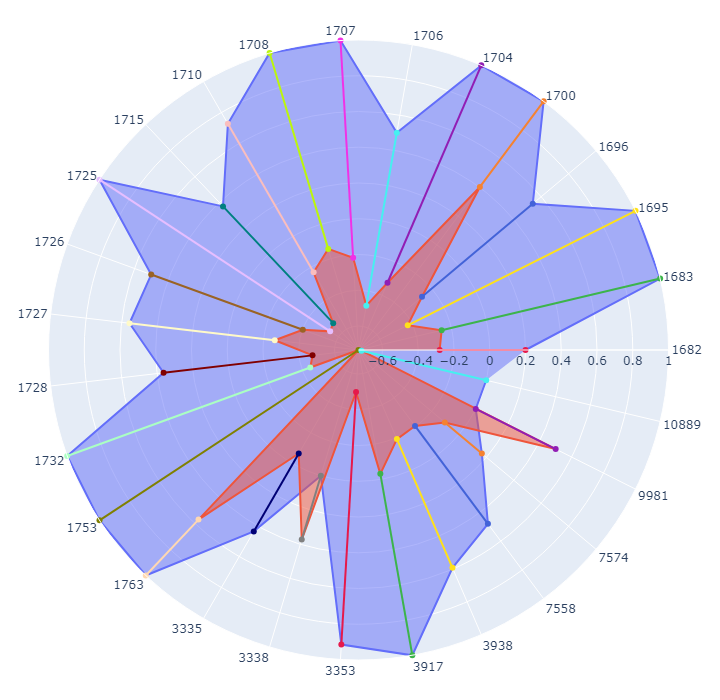
\includegraphics[width=0.7\textwidth]{images/social_barometer_homeland.png}
	\caption{Gráfico de Radar ilustrando a pressão social em relação ao tópico de Higienismo Urbano}
	\label{fig:social_barometer_homeland}
\end{figure}

\begin{table}[htbp]
	\centering
	\caption{Métricas de pressão social do tópico de Higienismo Urbano}
	\label{tab:eventos_populares_homeland}
	\begin{tabular}{|l|c|c|c|c|}
		\hline
		\textbf{Tipo de Evento}                               & \textbf{Eventos} & \textbf{Score} & \textbf{Persona} \\
		\hline
		7558:Ocupação irregular de área pública               & 11               & -0.2045        & 0.4783           \\
		\hline
		1715:Veículo abandonado                               & 8                & -0.5278        & 0.3704           \\
		\hline
		3938:Entulho na calçada/via pública                   & 8                & -0.1915        & 0.5930           \\
		\hline
		1708:Ponto de tráfico de drogas                       & 8                & -0.1438        & 1.0000           \\
		\hline
		3353:Aglomeração de pessoas                           & 7                & -0.4988        & 0.9167           \\
		\hline
		1696:Mato alto                                        & 7                & -0.2704        & 0.5385           \\
		\hline
		1710:Ponto de assalto/roubo                           & 7                & -0.2319        & 0.7273           \\
		\hline
		3335:Lâmpada apagada à noite                          & 5                & -0.0654        & 0.4375           \\
		\hline
		1728:Imóvel ou terreno abandonado                     & 5                & -0.4752        & 0.3636           \\
		\hline
		1725:Bloqueio na via                                  & 5                & -0.5444        & 1.0000           \\
		\hline
		1682:Estabelecimento com condição sanitária irregular & 4                & -0.2800        & 0.2000           \\
		\hline
		1726:Patrimônio histórico em risco                    & 3                & -0.4025        & 0.5000           \\
		\hline
		7574:Poda de árvore                                   & 3                & -0.1037        & 0.1667           \\
		\hline
		1704:Calçada inexistente                              & 3                & -0.3245        & 1.0000           \\
		\hline
		1706:Infestação animais perigosos                     & 2                & -0.4822        & 0.5000           \\
		\hline
		1700:Ponto de queimada irregular recorrente           & 2                & 0.4031         & 1.0000           \\
		\hline
		3917:Calçada irregular                                & 2                & -0.0305        & 1.0000           \\
		\hline
		1695:Praia suja                                       & 2                & -0.4259        & 1.0000           \\
		\hline
		3338:Iluminação pública irregular                     & 2                & 0.3730         & 0.0000           \\
		\hline
		9981:Atendimento no Posto de Saúde                    & 1                & 0.5002         & 0.0000           \\
		\hline
	\end{tabular}
\end{table}

Entretanto, é crucial observar que enquanto alguns usuários reportam eventos negativos relacionados a populações vulneráveis, outros demonstram preocupação e empatia. A menção de 'moradores de rua' 255 vezes, em contraste com palavras como 'vagabundos' ou 'vagabundo' (41 vezes no total), indica uma inclinação mais empática de muitos usuários. Contudo, a presença contínua de termos pejorativos nas postagens sugere que a polarização é real e persistente. A natureza binária desses sentimentos aponta para uma dicotomia na percepção pública: enquanto há um desejo coletivo de espaços públicos bem mantidos e seguros, também existe uma conscientização e, em muitos casos, uma preocupação genuína com as populações vulneráveis. Os relatórios sobre 'Calçada inexistente' ou 'Iluminação pública irregular' demonstram essa preocupação, pois tais problemas afetam diretamente a segurança e a acessibilidade nas cidades, impactando todos os cidadãos, mas especialmente os mais vulneráveis.

\begin{figure}[htb]
	\centering
	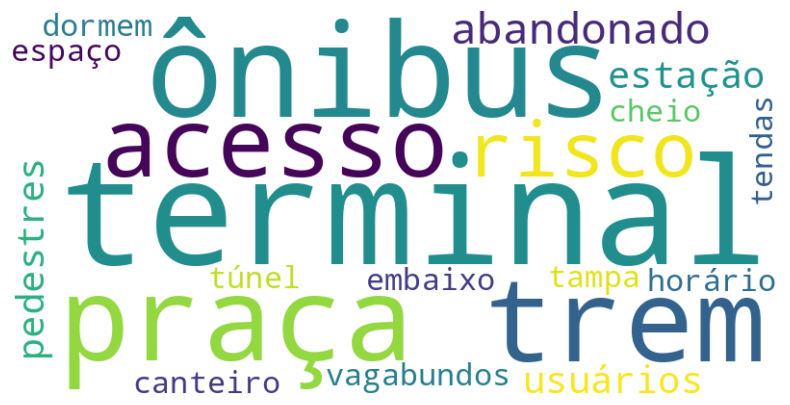
\includegraphics[width=0.7\textwidth]{images/wordcloud_homepand.png}
	\caption{Wordcloud com palavras mais frequentes em postagens sobre Higienismo Urbano}
	\label{fig:wordcloud_homepand}
\end{figure}

A dicotomia nos resultados demonstra um desafio para as cidades modernas: equilibrar o desejo por ordem e estética com a necessidade de justiça social e inclusão. O higienismo urbano e o design hostil são duas faces dessa moeda, e o conteúdo gerado por usuários de aplicativos como o Colab oferecem um vislumbre das opiniões e preocupações do público a respeito dessas questões.

\subsection{Segurança Pública}

O cenário urbano brasileiro tem experimentado uma série de transformações ao longo das últimas décadas, moldadas por fatores socioeconômicos, políticos e culturais. Dentre as diversas questões que emergem deste contexto, a segurança pública destaca-se como um dos tópicos mais sensíveis e debatidos. Em meio a desafios que vão desde a infraestrutura até a efetiva prestação de serviços públicos, a segurança é um termômetro que reflete não apenas a qualidade de vida dos cidadãos, mas também a estabilidade social de uma cidade ou região.

A segurança pública tornou-se um campo fértil para polarizações em grande parte devido à complexidade das causas e soluções associadas ao crime e à violência. Há aqueles que defendem abordagens mais repressivas e estratégias de 'tolerância zero', enquanto outros acreditam que o foco deveria estar em políticas sociais e prevenção. Essa divergência de opiniões frequentemente se traduz em tensões, com cada lado defendendo suas visões com paixão e, muitas vezes, resistência a abordagens alternativas. Muitas dessas opiniões polarizadoras sobre a segurança pública são informadas pelo alinhamento político dos indivíduos. Em linhas gerais, posições mais conservadoras tendem a favorecer abordagens punitivas e maior presença policial, enquanto posições mais progressistas tendem a enfatizar a necessidade de reformas sociais, educacionais e econômicas para abordar as causas subjacentes do crime. Essas perspectivas muitas vezes são alimentadas e amplificadas por líderes políticos, mídia e plataformas de redes sociais, criando câmaras de eco que reforçam crenças existentes.

A prevalência de um alto número de assaltos e roubos, como evidenciado pelos altos volumes de menções (assaltos: 619, roubos: 206), juntamente com uma persona predominantemente de complainer (scores negativos), reflete uma preocupação significativa com a criminalidade. Este achado é corroborado pela frequente menção de 'polícia' (284 vezes) e 'policiamento' (112 vezes), sugerindo uma demanda por maior segurança e vigilância. Por outro lado, a presença de helpers é menos proeminente nesses tópicos, talvez devido à natureza intrinsecamente problemática e desafiadora desses eventos, que podem não ser facilmente mitigados por ações comunitárias, ou seja, os usuários dependem do poder público para reagir a esses estímulos.

\begin{figure}[htb]
	\centering
	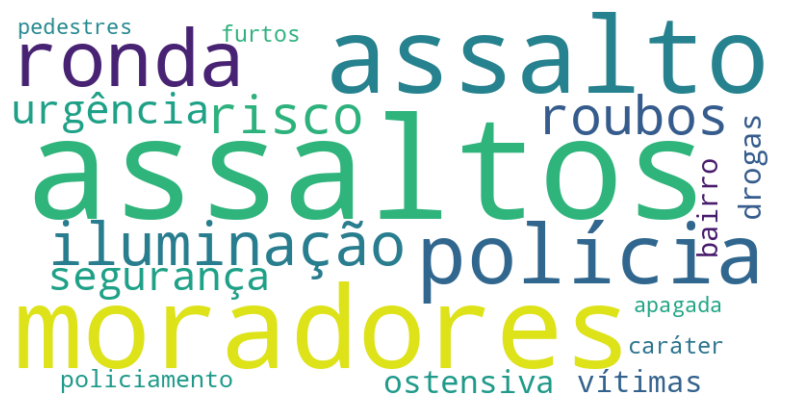
\includegraphics[width=0.7\textwidth]{images/wordcloud_security.png}
	\caption{Wordcloud com palavras mais frequentes em postagens sobre Segurança Pública}
	\label{fig:wordcloud_security}
\end{figure}

A análise dos scores de sentimentos e personas para cada tipo de evento fornece insights adicionais. Por exemplo, eventos como 'Ponto recorrente de poluição sonora' e 'Emissão de fumaça preta' demonstram sentimentos negativos expressos pelos usuários, que se inclinam majoritariamente para a persona \textit{complainer}. Este padrão sugere uma frustração considerável com questões ambientais e de qualidade de vida, onde os usuários expressam descontentamento mais do que propostas de soluções. Por outro lado, certos eventos apresentam um mix de personas, como é o caso do 'Imóvel ou terreno abandonado', indicando uma reação mais equilibrada entre reclamações e sugestões de melhoria. Tal equilíbrio sugere que, embora haja uma percepção negativa, existe também uma disposição para buscar soluções colaborativas.

Curiosamente, alguns eventos, como 'Bicicletário/paraciclo danificado', exibem um sentimento relativamente positivo, o que pode indicar uma resposta positiva da socidade ao reportar atos de vandalismo que danifiquem essas estruturas. No entanto, é importante notar que o volume desses relatos é significativamente menor em comparação com as categorias mais graves, como assaltos e roubos, mas ainda demonstram um hábito dos usuários de reportarem problemas relacionados ao vandalismo que afetam o patrimônio público. Ao examinar eventos como 'Pintura', 'Patrimônio histórico em risco' e 'Equipamento público danificado', observa-se um espectro variado de reações e envolvimentos da comunidade. No caso de 'Pintura', com um score de sentimento levemente positivo e uma persona mais próxima a \textit{helper} com uma alta incidência de termos como 'pichação' ou 'grafitti', sugere-se uma percepção da comunidade sobre a nuância desse tema e um sentimento mais coletivo de pertencimento sobre as estruturas públicas.

Em contrapartida, 'Patrimônio histórico em risco', com um score negativo acentuado e uma persona alta, indica uma forte reação negativa da comunidade. Isso reflete uma profunda preocupação com a preservação do patrimônio histórico, evidenciando a valorização cultural e a importância atribuída à conservação do legado histórico pela comunidade. A alta média \textit{complainer} neste caso sugere que os usuários estão mais propensos a adotar um crítico, denunciando problemas e muitas vezes mencionando órgaos públicos responsáveis, buscando chamar a atenção para o problema e exigir medidas de proteção e restauração. Por outro lado, 'Equipamento público danificado', com um score de sentimento ligeiramente negativo e uma persona moderada Estas observações revelam uma diversidade nas preocupações da comunidade em relação ao patrimônio público. Enquanto alguns aspectos, como a preservação do patrimônio histórico, mobilizam forte reação e engajamento, outros, como danos a equipamentos públicos ou questões estéticas como a pintura, geram reações menos intensas. Isso reflete a complexidade das percepções e prioridades dos cidadãos em relação ao espaço urbano e à sua conservação. É evidente que a comunidade valoriza aspectos culturais e históricos, demonstrando uma tendência a reagir de forma mais veemente e envolvida quando estes estão ameaçados, enquanto problemas menos simbólicos ou urgentes suscitam uma reação mais moderada.

\begin{figure}[htb]
	\centering
	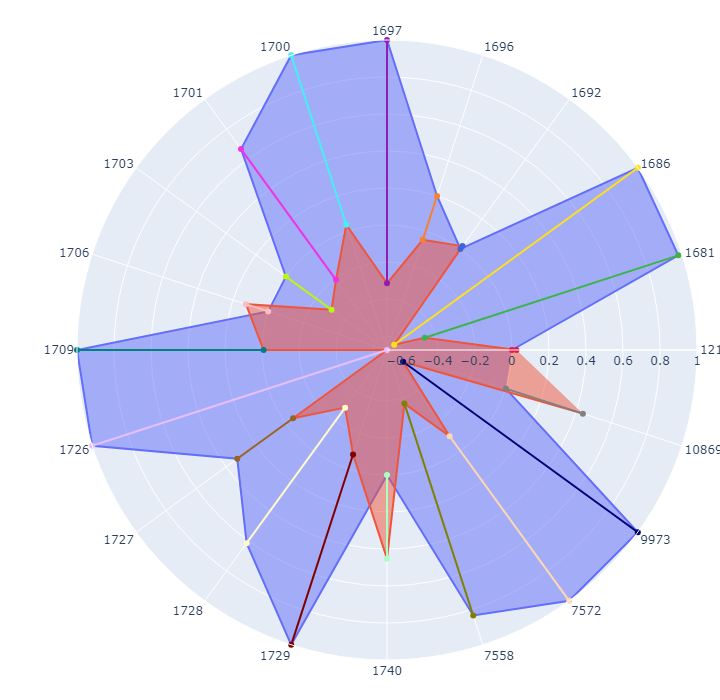
\includegraphics[width=0.7\textwidth]{images/social_barometer_security.png}
	\caption{Gráfico de Radar ilustrando a pressão social em relação ao tópico de Segurança Pública.}
	\label{fig:social_barometer_security}
\end{figure}

\begin{table}[htbp]
	\centering
	\caption{Métricas de pressão social do tópico de Segurança Pública}
	\label{tab:eventos_populares_security}
	\begin{tabular}{|l|c|c|c|c|}
		\hline
		\textbf{Tipo de Evento}                     & \textbf{Eventos} & \textbf{Score} & \textbf{Persona} \\
		\hline
		7558:Ocupação irregular de área pública     & 19               & -0.3704        & 0.8333           \\
		\hline
		1727:Equipamento público danificado         & 15               & -0.0478        & 0.3250           \\
		\hline
		1681:Ponto recorrente de poluição sonora    & 14               & -0.4606        & 0.9802           \\
		\hline
		1728:Imóvel ou terreno abandonado           & 12               & -0.2901        & 0.6154           \\
		\hline
		1696:Mato alto                              & 12               & -0.0493        & 0.2000           \\
		\hline
		1697:Maus tratos a animais                  & 7                & -0.3150        & 1.0000           \\
		\hline
		1701:Desmatamento irregular                 & 5                & -0.2063        & 0.6667           \\
		\hline
		9973:Má conduta de motorista ou cobrador    & 3                & -0.5674        & 1.0000           \\
		\hline
		1706:Infestação animais perigosos           & 3                & 0.1264         & 0.0000           \\
		\hline
		10869:Ônibus/trem/metrô danificado          & 2                & 0.4379         & 0.0000           \\
		\hline
		7572:Estabelecimento sem nota fiscal        & 1                & -0.0990        & 1.0000           \\
		\hline
		1740:Bicicletário/paraciclo danificado      & 1                & 0.4526         & 0.0000           \\
		\hline
		1729:Ponto de transporte clandestino        & 1                & -0.0816        & 1.0000           \\
		\hline
		121:Pintura                                 & 1                & 0.0247         & 0.0000           \\
		\hline
		1726:Patrimônio histórico em risco          & 1                & -0.6750        & 1.0000           \\
		\hline
		1703:Ponto de travessia irregular           & 1                & -0.3048        & 0.0000           \\
		\hline
		1700:Ponto de queimada irregular recorrente & 1                & 0.0365         & 1.0000           \\
		\hline
		1692:Lixeira quebrada                       & 1                & 0.0188         & 0.0000           \\
		\hline
		1686:Emissão de fumaça preta                & 1                & -0.6271        & 1.0000           \\
		\hline
		1709:Ponto de exploração sexual de menores  & 1                & -0.0083        & 1.0000           \\
		\hline
	\end{tabular}
\end{table}

Essa análise nos leva a inferir que, no espectro da pressão social relacionada à segurança pública, existe uma forte polarização. Por um lado, há uma expressiva vocalização de preocupações e frustrações, caracterizando um ambiente onde prevalecem as reclamações e a demanda por medidas mais efetivas. Por outro, observa-se uma participação proativa de uma parcela da comunidade, que, embora menor em número, sugere uma disposição para colaborar na identificação de soluções principalmente com respeito a crimes contra a estrutura pública da cidade e contra a vida.

Este cenário aponta para uma polarização significativa nos tópicos de segurança pública, com uma inclinação predominante para reações negativas e críticas. Os cidadãos parecem mais propensos a vocalizar insatisfações e preocupações em vez de sugerir soluções ou colaborar para melhorias, o que pode ser um reflexo da percepção de que esses problemas estão além do controle e influência diretos da comunidade. A predominância de personas de complainers em muitos dos eventos analisados sugere uma sensação de desamparo e frustração com as questões de segurança pública, contrastando com a presença menos frequente de helpers, que tendem a se concentrar em questões mais gerenciáveis.

A conclusão que emerge desses dados é a de uma comunidade ativamente engajada nas questões de segurança pública, mas cujo engajamento é predominantemente orientado para a expressão de preocupações e demandas por ação. Isso sinaliza uma oportunidade para os tomadores de decisão e as autoridades locais de capitalizar sobre essa participação ativa, canalizando-a para iniciativas colaborativas de segurança e melhorias urbanas. Ao mesmo tempo, revela um desafio significativo em termos de gestão e resposta às expectativas dos cidadãos, exigindo uma abordagem que equilibre a resposta imediata às preocupações com a promoção de um diálogo construtivo que inclua todas as vozes da comunidade.

\subsection{Política de Drogas}

O problema das drogas nos espaços urbanos do Brasil é um tema complexo, marcado por inúmeras facetas que interagem de formas intrincadas. Esse problema não apenas toca a saúde pública e a segurança, mas também permeia questões sociais, econômicas e políticas. O Brasil, com suas grandes cidades e desigualdades socioeconômicas acentuadas, apresenta um cenário em que o uso e o tráfico de drogas se tornam questões centrais em diversas discussões urbanas.

A política de drogas é um assunto que gera polarização intensa, principalmente porque ele abrange uma gama de perspectivas que vão desde o rigoroso controle e penalização até abordagens mais liberais e focadas na saúde pública. Essa polarização surge em parte devido às diferenças ideológicas sobre como a sociedade deve lidar com as drogas e seus usuários. Alguns argumentam que a guerra às drogas falhou, propondo uma abordagem mais focada na prevenção e no tratamento, enquanto outros defendem políticas mais duras, visando a repressão ao tráfico e ao consumo.

\begin{figure}[htb]
	\centering
	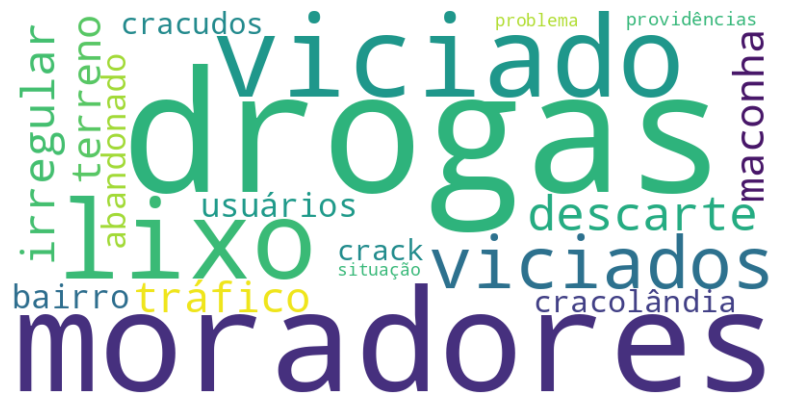
\includegraphics[width=0.7\textwidth]{images/wordcloud_drugs.png}
	\caption{Wordcloud com palavras mais frequentes em postagens sobre Política de Drogas}
	\label{fig:wordcloud_drugs}
\end{figure}

Quando analisamos como os usuários do aplicativo Colab percebem o problema das drogas, fica evidente que eles refletem essa polarização. Por um lado, alguns usuários podem ver o uso de drogas como um problema de saúde pública, enfatizando a necessidade de tratamento e apoio aos dependentes químicos. Por outro lado, há aqueles que o enxergam principalmente como uma questão de segurança pública, associando o uso e o tráfico de drogas à criminalidade e à degradação urbana.

A maneira como os usuários do Colab se referem aos usuários de drogas oferece uma janela para entender sua percepção sobre o tema. Palavras como 'drogado', 'viciado' e 'cracudo' carregam conotações fortemente negativas e estigmatizantes, sugerindo que muitos usuários do aplicativo podem ver o uso de drogas mais como um vício moral ou uma escolha individual errada do que como uma questão de saúde. Isso pode refletir uma tendência a responsabilizar o indivíduo pelo uso de drogas, em vez de considerar o contexto social e econômico mais amplo.

No que diz respeito à relação entre os problemas de zeladoria pública e as menções a drogas, é possível que os usuários do Colab estejam associando a presença de usuários de drogas com a negligência e o abandono urbano. Por exemplo, um imóvel ou terreno abandonado pode ser visto como um local propício para o consumo de drogas. Da mesma forma, áreas com mato alto ou estruturas quebradas podem ser percebidas como negligenciadas pela administração pública, tornando-se espaços onde atividades ilegais, incluindo o uso e o tráfico de drogas, possam ocorrer sem supervisão.

\begin{figure}[htb]
	\centering
	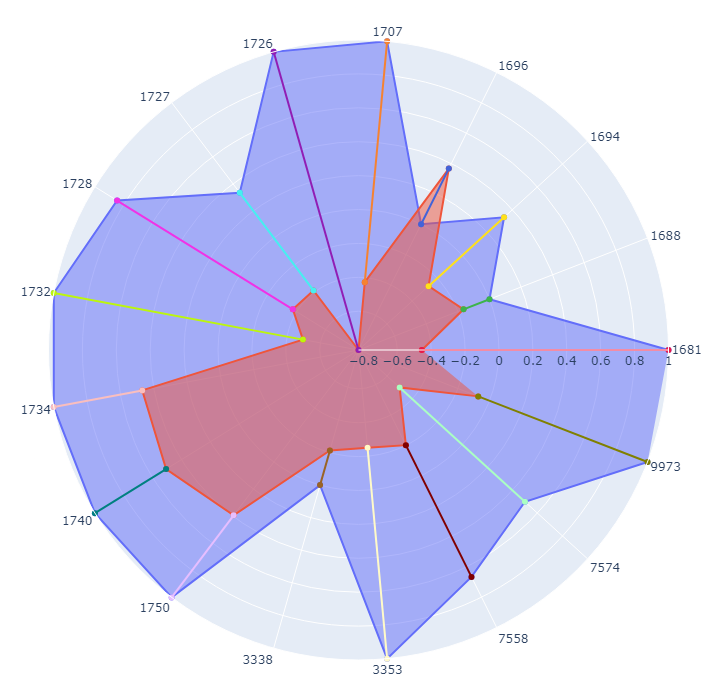
\includegraphics[width=0.7\textwidth]{images/social_barometer_drugs.png}
	\caption{Gráfico de Radar ilustrando a pressão social em relação ao tópico de Política de Drogas.}
	\label{fig:social_barometer_drugs}
\end{figure}

\begin{table}[htbp]
	\centering
	\caption{Métricas de pressão social do tópico de Política de Drogas}
	\label{tab:eventos_populares_drugs}
	\begin{tabular}{|l|c|c|c|c|}
		\hline
		\textbf{Tipo de Evento}                  & \textbf{Eventos} & \textbf{Score} & \textbf{Persona} \\
		\hline
		7558:Ocupação irregular de área pública  & 11               & -0.2017        & 0.6667           \\
		\hline
		1728:Imóvel ou terreno abandonado        & 10               & -0.3732        & 0.8462           \\
		\hline
		1727:Equipamento público danificado      & 9                & -0.3882        & 0.3333           \\
		\hline
		3353:Aglomeração de pessoas              & 6                & -0.2493        & 1.0000           \\
		\hline
		1694:Descarte irregular de lixo          & 5                & -0.2694        & 0.3333           \\
		\hline
		1696:Mato alto                           & 5                & 0.3668         & 0.0000           \\
		\hline
		1726:Patrimônio histórico em risco       & 5                & -0.8286        & 1.0000           \\
		\hline
		7574:Poda de árvore                      & 5                & -0.5005        & 0.5000           \\
		\hline
		1681:Ponto recorrente de poluição sonora & 3                & -0.4550        & 1.0000           \\
		\hline
		1707:Foco de mosquito da dengue/zika     & 3                & -0.4270        & 1.0000           \\
		\hline
		1688:Falta de energia                    & 2                & -0.1643        & 0.0000           \\
		\hline
		3338:Iluminação pública irregular        & 1                & -0.2125        & 0.0000           \\
		\hline
		1732:Área com risco de deslizamento      & 1                & -0.4953        & 1.0000           \\
		\hline
		1750:Varrição                            & 1                & 0.3936         & 1.0000           \\
		\hline
		1740:Bicicletário/paraciclo danificado   & 1                & 0.5062         & 1.0000           \\
		\hline
		1734:Retirada de árvore                  & 1                & 0.4690         & 1.0000           \\
		\hline
		9973:Má conduta de motorista ou cobrador & 1                & -0.0712        & 1.0000           \\
		\hline
	\end{tabular}
\end{table}

Essas associações podem ser influenciadas pelo que é frequentemente retratado na mídia, onde locais em deterioração urbana são comumente associados ao uso de drogas. Por isso, quando usuários do Colab relatam problemas de zeladoria e mencionam drogas, eles podem estar refletindo essa narrativa. Isso é evidenciado pelo fato de que problemas associados a uma alta persona R e scores R negativos, como 'Patrimônio histórico em risco' ou 'Foco de mosquito da dengue/zika', frequentemente recebem menções a drogas, sugerindo uma percepção de que esses problemas são exacerbados ou até causados pela presença de usuários de drogas.

Além disso, essa percepção está alinhada com a ideia de que áreas negligenciadas pela administração pública podem se tornar focos de problemas sociais mais amplos, incluindo o uso de drogas. Isso reflete um ciclo vicioso: locais abandonados atraem atividades ilícitas, o que por sua vez contribui para mais abandono e deterioração. A menção de drogas nessas descrições de problemas urbanos no Colab pode, portanto, estar destacando essa dinâmica, onde o uso de drogas é tanto uma consequência quanto um fator contribuinte para a degradação urbana.

Esse fenômeno aponta para a necessidade de uma abordagem holística na gestão urbana, que não só aborde o problema das drogas em si, mas também as condições sociais e urbanas que favorecem o seu uso. Tal abordagem envolveria não apenas medidas de segurança e saúde pública, mas também investimentos em infraestrutura, revitalização de áreas degradadas e programas de inclusão social.

Portanto, a análise dos dados do Colab revela como os cidadãos percebem e interagem com o problema das drogas nas cidades brasileiras. Ela mostra uma tendência a associar o uso de drogas com problemas urbanos, enfatizando a necessidade de soluções que abordem tanto as questões de saúde pública quanto as condições sociais e ambientais que facilitam o uso de drogas. Assim, enquanto o debate sobre a política de drogas continua a ser uma fonte de polarização, é essencial considerar como as diferentes percepções e experiências dos cidadãos podem informar e influenciar essas políticas. A resposta ao problema das drogas, portanto, exige uma abordagem integrada que considere tanto as nuances individuais quanto os fatores estruturais e sociais em jogo.

\subsection{Pânico Moral}

O conceito de 'pânico moral', conforme delineado por Stanley Cohen em sua obra seminal 'Folk Devils and Moral Panics' (1972), fornece um quadro interpretativo valioso para compreender como certas questões sociais e comportamentos são amplificados e distorcidos dentro do discurso público, levando à criação de 'bodes expiatórios' ou 'demônios sociais'. No contexto brasileiro contemporâneo, e especialmente através de plataformas interativas como o Colab, podemos observar a manifestação desse fenômeno de forma peculiar. Cohen descreve o pânico moral como uma reação da sociedade a um grupo ou subcultura percebida como ameaçadora aos valores e interesses sociais estabelecidos. Essa dinâmica é frequentemente caracterizada por uma distorção e exagero na percepção da ameaça. No Colab, essas expressões de pânico moral podem ser particularmente reveladoras, proporcionando uma janela para entender como certas preocupações são moldadas e amplificadas no espaço digital.

Por exemplo, reclamações sobre poluição sonora, especialmente relacionadas a gêneros musicais como o funk e o pagode, podem refletir não apenas preocupações legítimas com o ruído, mas também preconceitos culturais e sociais. Isso se alinha com a noção de Cohen sobre a criação de 'bodes expiatórios', onde determinados estilos musicais e seus apreciadores são estigmatizados, representando mais do que uma mera perturbação sonora, mas sim uma ameaça à ordem e aos valores sociais.

\begin{figure}[htb]
	\centering
	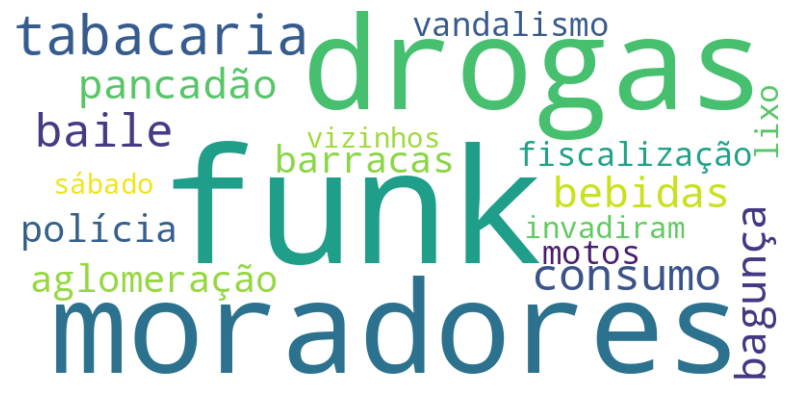
\includegraphics[width=0.7\textwidth]{images/wordcloud_moral.png}
	\caption{Wordcloud com palavras mais frequentes em postagens sobre Pânico Moral}
	\label{fig:wordcloud_moral}
\end{figure}

Além disso, o uso de termos pejorativos e discriminatórios em postagens relativas a eventos de zeladoria pública ou questões LGBTQIA+ pode sinalizar a presença de um pânico moral. Nesse contexto, grupos ou comportamentos são retratados de maneira distorcida, contribuindo para a disseminação de estereótipos e a marginalização de minorias. A presença de tais termos no Colab sugere que essas atitudes não estão restritas a esferas privadas ou conversas informais, mas se infiltram em discussões públicas sobre a gestão urbana e social.

A análise desses padrões de comunicação no Colab pode fornecer insights valiosos sobre as tensões subjacentes na sociedade brasileira. Permite aos pesquisadores e formuladores de políticas entender melhor não apenas as preocupações práticas dos cidadãos, mas também as dinâmicas psicossociais e culturais que moldam a percepção pública de certos grupos e questões. Ao identificar e analisar manifestações de pânico moral na plataforma, é possível adotar uma abordagem mais informada e matizada para enfrentar tanto as questões práticas da vida urbana quanto os desafios mais amplos de integração social e tolerância.

Ao analisar os resultados de pressão social, encontramos evidências claras de uma polarização relacionada à música, especialmente ao pagode e ao funk. Essa polarização é evidenciada pelos eventos de 'Ponto recorrente de poluição sonora' e 'Emissão de fumaça preta'. Ambos os eventos têm uma persona média predominantemente \textit{complainer}. Isso sugere que os usuários tendem a adotar uma abordagem crítica e insatisfeita em relação a eventos de poluição sonora, possivelmente devido ao impacto negativo do barulho, que frequentemente está associado a festas de pagode e funk. Essa conexão entre música e eventos de zeladoria pública demonstra um claro preconceito musical e uma polarização em relação a esses gêneros, que são percebidos negativamente por alguns membros da comunidade.

Além disso, as palavras-chave identificadas, como 'narguile', 'tabacaria' e 'grafite', sugerem que os usuários também estão associando comportamentos como fumar narguilé e grafites a eventos de zeladoria pública. Essas associações parecem ser negativas, pois esses eventos têm persona média predominantemente \textit{complainer}, refletindo a preocupação ou descontentamento dos usuários em relação a esses comportamentos. Essa conexão entre eventos culturais e preocupações com a zeladoria pública indica que a plataforma está sendo usada para expressar opiniões e críticas sobre questões culturais e comportamentais, além das questões de infraestrutura tradicionais.

Outro aspecto importante a ser destacado é a associação entre eventos de zeladoria pública, como 'Fiação irregular', 'Ocupação irregular de área pública' e 'Construção irregular', e os eventos culturais mencionados anteriormente, como bailes de funk e pagode. Os usuários parecem se incomodar com o barulho e a informalidade desses eventos e, como resultado, criam eventos de zeladoria pública para relatar irregularidades e tentar fechar esses estabelecimentos. Essa estratégia sugere uma tentativa de utilizar as ferramentas disponíveis na plataforma para influenciar o fechamento desses locais, refletindo uma tentativa de impor normas sociais e urbanas.

\begin{figure}[htb]
	\centering
	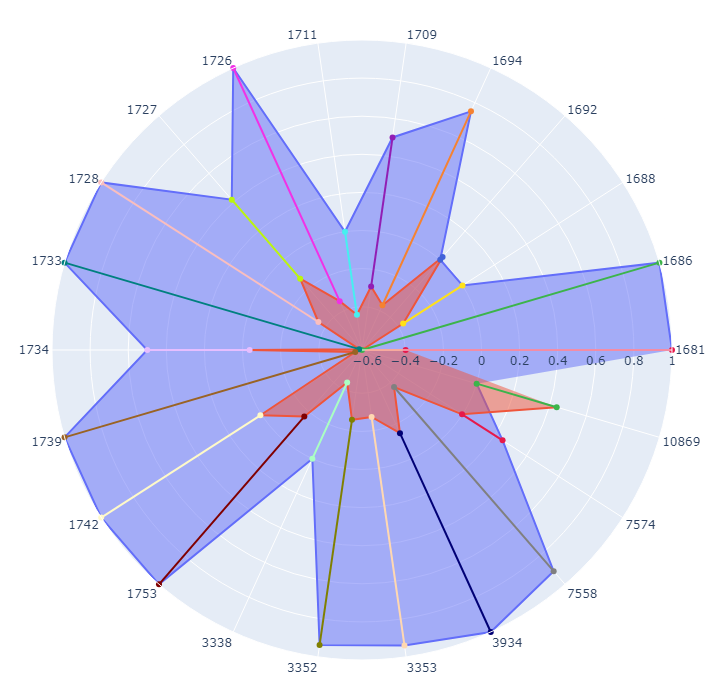
\includegraphics[width=0.7\textwidth]{images/social_barometer_moral.png}
	\caption{Gráfico de Radar ilustrando a pressão social em relação ao tópico de Pânico Moral.}
	\label{fig:social_barometer_moral}
\end{figure}

\begin{table}[htbp]
	\centering
	\caption{Métricas de pressão social do tópico de Pânico Moral}
	\label{tab:eventos_populares_moral_panic}
	\begin{tabular}{|l|c|c|c|c|}
		\hline
		\textbf{Tipo de Evento}                    & \textbf{Eventos} & \textbf{Score} & \textbf{Persona} \\
		\hline
		1681:Ponto recorrente de poluição sonora   & 9                & -0.3983        & 1.0000           \\
		\hline
		3353:Aglomeração de pessoas                & 9                & -0.2718        & 0.9394           \\
		\hline
		7558:Ocupação irregular de área pública    & 8                & -0.3703        & 0.9091           \\
		\hline
		3352:Comércio aberto irregularmente        & 7                & -0.2571        & 0.9375           \\
		\hline
		1694:Descarte irregular de lixo            & 5                & -0.3687        & 0.7500           \\
		\hline
		1739:Evento Irregular                      & 5                & -0.5900        & 1.0000           \\
		\hline
		1728:Imóvel ou terreno abandonado          & 4                & -0.3551        & 1.0000           \\
		\hline
		7574:Poda de árvore                        & 3                & -0.0028        & 0.2500           \\
		\hline
		1727:Equipamento público danificado        & 3                & -0.1315        & 0.4167           \\
		\hline
		1726:Patrimônio histórico em risco         & 2                & -0.3454        & 1.0000           \\
		\hline
		1753:Construção irregular                  & 1                & -0.1647        & 1.0000           \\
		\hline
		3934:Fiação irregular                      & 1                & -0.1474        & 1.0000           \\
		\hline
		3338:Iluminação pública irregular          & 1                & -0.4396        & 0.0000           \\
		\hline
		1734:Retirada de árvore                    & 1                & -0.0372        & 0.5000           \\
		\hline
		1742:Vazamento de esgoto                   & 1                & 0.0068         & 1.0000           \\
		\hline
		1686:Emissão de fumaça preta               & 1                & -0.6271        & 1.0000           \\
		\hline
		1733:Publicidade irregular em via pública  & 1                & -0.6114        & 1.0000           \\
		\hline
		1711:Ponto de ônibus danificado            & 1                & -0.4399        & 0.0000           \\
		\hline
		1709:Ponto de exploração sexual de menores & 1                & -0.2906        & 0.5000           \\
		\hline
		1692:Lixeira quebrada                      & 1                & 0.0188         & 0.0000           \\
		\hline
	\end{tabular}
\end{table}

A associação entre eventos culturais e eventos de zeladoria pública também é evidente nas métricas de pressão social. Os eventos de 'Comércio aberto irregularmente', 'Aglomeração de pessoas' e 'Evento Irregular' têm persona média equilibrada entre \textit{helper} e \textit{complainers}. Isso indica uma diversidade de opiniões em relação a esses eventos, possivelmente refletindo a complexidade do tópico e as diferentes perspectivas dos usuários. Essa diversidade sugere que, enquanto alguns usuários estão preocupados com a infração das regras e o impacto negativo na comunidade, outros podem ver esses eventos como oportunidades culturais ou econômicas.

Além disso, a questão da informalidade na organização desses eventos culturais, como mencionado com bailes de funk e pagode, é uma preocupação subjacente. Os eventos de 'Imóvel ou terreno abandonado' e 'Patrimônio histórico em risco' também refletem uma persona média predominantemente \textit{complainer}. Isso sugere que os usuários frequentemente expressam insatisfação em relação à falta de preservação do patrimônio histórico e à presença de imóveis ou terrenos abandonados, possivelmente relacionando essas questões à informalidade e ao descuido urbanos.

No entanto, é importante notar que, apesar da polarização evidente em relação a eventos culturais e comportamentais, outros eventos, como 'Lixeira quebrada', 'Descarte irregular de lixo' e 'Poda de árvore', têm persona média mais equilibrada, sugerindo que os usuários tendem a adotar uma postura mais colaborativa e positiva em relação a essas questões de infraestrutura.

Em relação à questão da polarização, os resultados indicam que a música, especialmente os gêneros de pagode e funk, parece ser um ponto sensível que gera opiniões polarizadas. Isso pode ser atribuído a uma série de fatores, incluindo preconceito musical, percepções culturais e experiências pessoais. Além disso, a associação de comportamentos como fumar narguilé e grafites a eventos de zeladoria pública demonstra como as preocupações urbanas podem ser interligadas a aspectos culturais e comportamentais.

A questão da informalidade na organização desses eventos culturais também é notável. Os usuários parecem preocupados com a falta de regulamentação e controle em torno desses eventos, o que os leva a relatar problemas de infraestrutura e irregularidades para tentar influenciar o fechamento desses estabelecimentos. Isso pode refletir uma tentativa de impor normas sociais e urbanas por meio da plataforma Colab. Além disso, é importante destacar a relevância do evento 'Ocupação irregular de área pública', que possui uma persona média predominantemente \textit{helper}. Isso sugere que os usuários estão ativamente envolvidos em relatar ocupações irregulares de áreas públicas e trabalhar para resolver esse problema. Essa é uma indicação positiva de participação cidadã na plataforma.

A análise das métricas de pressão social no Colab revela não apenas a polarização significativa em relação a eventos culturais e comportamentos associados, mas também lança luz sobre a existência de um fenômeno que pode ser caracterizado como 'pânico moral'. O pânico moral ocorre quando a sociedade reage de forma exagerada e moralista a determinados comportamentos ou eventos, muitas vezes atribuindo a eles uma ameaça à ordem social e aos valores tradicionais. Nesse contexto, a polarização em torno de eventos culturais como festas de pagode e funk, bem como comportamentos como fumar narguilé e grafites, reflete não apenas as preferências individuais, mas também preconceitos musicais e percepções culturais profundamente enraizadas. Os usuários do Colab estão expressando suas opiniões de forma polarizada, com alguns adotando uma postura crítica e outros buscando colaborar na resolução dessas questões.

A análise das personas médias e scores médios é fundamental para chegarmos a essa conclusão. A persona média nos ajuda a entender como os usuários se comportam e se relacionam com os eventos de zeladoria pública, enquanto o score médio de sentimento nos fornece uma medida objetiva das opiniões expressas. A combinação dessas métricas permite uma compreensão mais completa das dinâmicas sociais e das percepções dos usuários. Essas informações têm implicações importantes para stakeholders, como governos municipais e organizações da sociedade civil. Primeiramente, eles podem usar essas análises para compreender as preocupações e perspectivas dos cidadãos em relação a eventos de zeladoria pública específicos. Isso pode ajudar na formulação de políticas e estratégias mais alinhadas com as necessidades da comunidade.

A identificação do pânico moral em torno de certos tópicos culturais pode levar a esforços educacionais e de conscientização. Os stakeholders podem trabalhar para promover um diálogo mais informado e inclusivo sobre esses temas, reduzindo a polarização e fomentando uma compreensão mútua. Em conclusão, a análise das métricas de pressão social no Colab não apenas oferece insights valiosos sobre as preocupações urbanas e sociais, mas também sugere oportunidades para a construção de comunidades mais informadas e colaborativas, onde as divergências são tratadas com empatia e compreensão.

\subsection{Política Tributária}

No contexto das discussões sobre questões urbanas, observamos a presença recorrente de argumentos que abordam a questão dos altos impostos municipais e estaduais, assim como os custos associados aos serviços públicos oferecidos à população. Esses argumentos frequentemente destacam a relação intrínseca entre a carga tributária e a qualidade dos serviços públicos. Além disso, os usuários também levantam questões relacionadas à corrupção e à má gestão dos recursos públicos, que podem ser diretamente associadas à política tributária. A análise dos eventos relacionados a essa temática revela uma tendência marcante: a maioria deles exibe scores médios negativos. Essa tendência sugere que os usuários tendem a expressar sentimentos predominantemente negativos em relação a eventos vinculados a impostos, como o IPTU e IPVA. Essa predominância de sentimentos negativos pode indicar um profundo descontentamento em relação à carga tributária vigente ou à forma como os impostos são administrados.

Entretanto, é importante observar que a associação direta entre o aumento de impostos e a deterioração dos serviços públicos pode representar uma falácia lógica, conhecida como 'falácia post hoc' ou 'falácia da causalidade'. Esta falácia ocorre quando se assume erroneamente que, porque um evento ocorreu antes de outro, o primeiro evento foi a causa do segundo. Nesse contexto, a falácia post hoc ocorre quando os usuários atribuem a piora dos serviços públicos unicamente ao aumento dos impostos, sem considerar outros fatores relevantes. É fundamental reconhecer que a relação entre a carga tributária e a qualidade dos serviços públicos é complexa e influenciada por uma série de variáveis, como gestão pública, alocação de recursos, políticas governamentais e eficiência administrativa. Portanto, é imperativo adotar uma abordagem mais abrangente e holística para compreender a interação entre impostos e serviços públicos. Essa abordagem deve considerar não apenas os aspectos relacionados à política tributária, mas também examinar outros fatores que podem afetar a prestação de serviços públicos de qualidade. Além disso, é essencial evitar generalizações simplistas que podem levar a discursos polarizados e à disseminação de informações imprecisas. Ao analisar criticamente as questões urbanas e a política tributária, os usuários podem contribuir de maneira mais construtiva para o debate público e para a formulação de políticas que busquem a melhoria da qualidade de vida nas cidades.

\begin{figure}[htb]
	\centering
	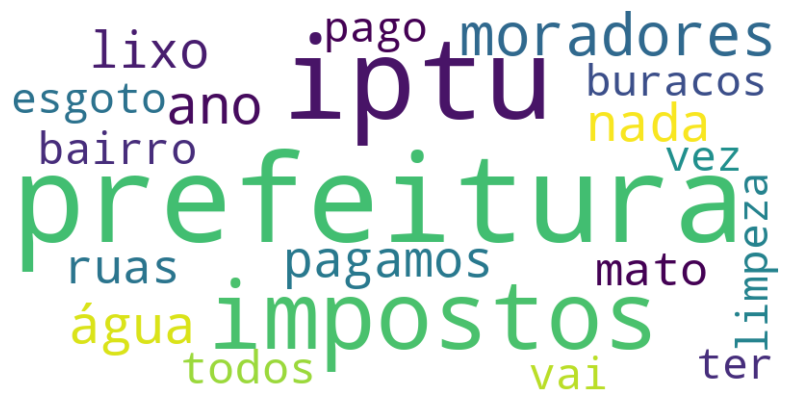
\includegraphics[width=0.7\textwidth]{images/wordcloud_taxes.png}
	\caption{Wordcloud com palavras mais frequentes em postagens sobre Política Tributária}
	\label{fig:wordcloud_taxes}
\end{figure}

Nesse contexto, investigar as dinâmicas de pressão social relacionadas à política tributária e às questões urbanas, a fim de compreender melhor como os usuários do Colab se engajam nesse debate e como suas opiniões e sentimentos se manifestam. Ao explorar os eventos selecionados e as métricas de pressão social associadas a eles, buscamos identificar tendências, padrões e possíveis polarizações nas discussões sobre impostos e serviços públicos. Notavelmente, constatamos que, quando a persona dos usuários é identificada como \textit{complainer}, denotando uma tendência a expressar reclamações ou insatisfações individualistas, e o score de sentimento da postagem é majoritariamente negativo muitos usuários fazem referência a termos tributários, como IPTU, impostos e IPVA, em suas postagens. Essa observação sugere que, em grande parte, os usuários utilizam os impostos como justificativa para expressar seu descontentamento em relação à qualidade dos serviços públicos, argumentando que, considerando a quantidade de impostos pagos, os serviços deveriam ser de melhor qualidade. Essa análise crítica permitirá uma visão mais informada sobre as preocupações dos cidadãos em relação à política tributária e contribuirá para um diálogo mais substancial e equilibrado sobre esse tema de relevância pública.

Para uma análise mais detalhada dos resultados do Barômetro de Pressão Social relacionados à política tributária, procedemos à categorização dos eventos em seis áreas distintas: transporte público, infraestrutura e patrimônio público, meio ambiente, saneamento básico, iluminação e energia, e saúde pública. Cada uma dessas categorias abrange eventos que foram mencionados pelos usuários e apresenta uma perspectiva única sobre como a política tributária é percebida em relação a diferentes serviços públicos e questões urbanas. As avaliações de persona e score foram realizadas para cada categoria, permitindo uma compreensão mais profunda das preocupações e sentimentos dos usuários em relação a esses tópicos específicos. A seguir, exploraremos os resultados dessas categorias e suas implicações em relação à percepção pública sobre impostos e serviços públicos.

No que diz respeito ao transporte público, os eventos relacionados a problemas como 'ônibus superlotado' 'ponto de ônibus danificado' e 'ônibus fora do horário/rota' exibem persona média próxima \textit{complainer} e scores médios negativos. Isso sugere que os usuários tendem a reclamar dessas questões, expressando sentimentos predominantemente negativos. Essas reclamações podem estar relacionadas aos altos impostos pagos pelos cidadãos. Os usuários podem argumentar que, dado o montante de impostos que pagam, esperam um serviço de transporte público de maior qualidade. Portanto, há uma correlação entre reclamações sobre transporte público e insatisfação com a política tributária, na medida em que os impostos podem ser vistos como financiadores dos serviços de transporte.

Quando examinamos eventos relacionados à infraestrutura e patrimônio público, como 'buraco nas vias' 'estação de ônibus/trem/metrô danificada' 'fiação irregular' e 'patrimônio histórico em risco' observamos uma persona média próxima \textit{complainer} e scores médios negativos. Isso indica que os usuários tendem a reclamar dessas questões e expressar sentimentos predominantemente negativos. É interessante notar que, nesse contexto, a reclamação não está diretamente relacionada aos impostos, mas sim à qualidade dos serviços públicos e à conservação da infraestrutura. No entanto, há uma conexão indireta com a política tributária, uma vez que os cidadãos podem questionar a alocação de recursos e a eficácia do gasto público, considerando os impostos que pagam.

Ao examinar eventos de Meio Ambiente, como 'Vazamento de água' e 'Mato alto', apresentam scores médios negativos, indicando uma tendência de sentimentos negativos entre os usuários. No entanto, a persona média é próxima de 1, o que sugere uma inclinação mais forte para o perfil \textit{complainer}. Nesse contexto, os usuários podem estar insatisfeitos com a gestão dos recursos públicos e, possivelmente, associando essa insatisfação aos impostos pagos.

\begin{figure}[htb]
	\centering
	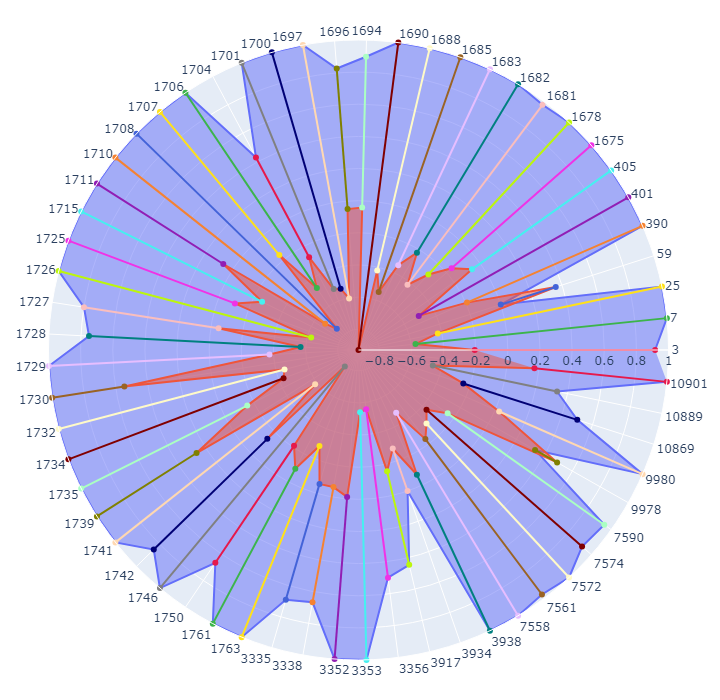
\includegraphics[width=0.7\textwidth]{images/social_barometer_taxes.png}
	\caption{Gráfico de Radar ilustrando a pressão social em relação ao tópico de Política Tributária.}
	\label{fig:social_barometer_taxes}
\end{figure}

\begin{table}[htbp]
	\centering
	\caption{Métricas de pressão social do tópico de Política Tributária}
	\label{tab:eventos_populares_taxes}
	\begin{tabular}{|l|c|c|c|c|}
		\hline
		\textbf{Tipo de Evento}                               & \textbf{Eventos} & \textbf{Score} & \textbf{Persona} \\
		\hline
		1694:Descarte irregular de lixo                       & 9                & -0.0427        & 0.8966           \\
		\hline
		3:Buraco nas vias                                     & 8                & -0.2060        & 0.9167           \\
		\hline
		3917:Calçada irregular                                & 7                & -0.1545        & 0.4444           \\
		\hline
		7:Ponto de infração de trânsito recorrente            & 6                & -0.5726        & 1.0000           \\
		\hline
		7574:Poda de árvore                                   & 6                & -0.3658        & 0.9231           \\
		\hline
		1696:Mato alto                                        & 6                & -0.0494        & 0.8276           \\
		\hline
		3938:Entulho na calçada/via pública                   & 6                & -0.0718        & 1.0000           \\
		\hline
		1678:Falta de água                                    & 6                & -0.2894        & 1.0000           \\
		\hline
		3335:Lâmpada apagada à noite                          & 6                & -0.0613        & 0.6897           \\
		\hline
		1715:Veículo abandonado                               & 5                & -0.2586        & 1.0000           \\
		\hline
		1727:Equipamento público danificado                   & 5                & -0.0481        & 0.8000           \\
		\hline
		1735:Via de terra com desnível                        & 5                & -0.1554        & 1.0000           \\
		\hline
		3338:Iluminação pública irregular                     & 5                & -0.0619        & 0.6667           \\
		\hline
		1683:Estabelecimento sem alvará                       & 5                & -0.3461        & 1.0000           \\
		\hline
		1682:Estabelecimento com condição sanitária irregular & 5                & -0.2227        & 1.0000           \\
		\hline
		7590:Bueiro entupido                                  & 5                & -0.2488        & 0.9474           \\
		\hline
		25:Vazamento de água                                  & 5                & -0.4253        & 1.0000           \\
		\hline
		1750:Varrição                                         & 4                & -0.2105        & 0.6667           \\
		\hline
		7558:Ocupação irregular de área pública               & 4                & -0.4740        & 1.0000           \\
		\hline
		1742:Vazamento de esgoto                              & 4                & -0.1369        & 0.8500           \\
		\hline
	\end{tabular}
\end{table}

Eventos relacionados ao saneamento básico, como 'Esgoto a céu aberto' e 'Bueiro entupido', também demonstram scores médios negativos, sugerindo uma insatisfação geral em relação a esses problemas urbanos. A persona média, novamente, tende a ser próxima de 1, o que indica que os usuários estão mais propensos a serem \textit{complainers}. A presença de termos como 'impostos' ou 'iptu' em postagens relacionadas a esses eventos sugere que os usuários estão usando a questão tributária como argumento para exigir melhorias nos serviços de saneamento.

Quando se trata de eventos como 'Lâmpada apagada à noite' e 'Iluminação pública irregular', observamos scores médios negativos. Novamente, a persona média tende a se aproximar de um perfil mais inclinado a ser \textit{complainer}. A presença de termos relacionados a impostos sugere que os usuários podem estar associando a má qualidade desses serviços públicos à política tributária, expressando descontentamento.

Eventos relacionados à saúde pública, como 'Atendimento na Clínica da Família', apresentam scores positivos, indicando sentimentos mais positivos entre os usuários. No entanto, a persona média tende a ser próxima de 1, sugerindo que, mesmo ao expressar sentimentos positivos, os usuários ainda podem ter inclinação para o perfil \textit{complainer}. Nesse contexto, a menção ocasional de termos como 'impostos' ou 'gestão pública' pode indicar que os usuários estão conscientes das questões fiscais relacionadas à saúde pública, mas podem estar dispostos a elogiar melhorias percebidas.

É fundamental destacar que, em todos os casos, a conexão direta entre a insatisfação em relação aos serviços públicos e o aumento de impostos pode ser uma simplificação excessiva da intrincada relação entre tributação e oferta de serviços. Embora os scores médios negativos indiquem claramente insatisfação, é imperativo considerar outros fatores, como má gestão, alocação de recursos e eficiência administrativa, que também podem desempenhar papéis significativos na qualidade dos serviços públicos. Além disso, a persona média próxima de 1, sugerindo uma inclinação para o perfil \textit{complainer}, aponta para a possibilidade de que os usuários estejam usando a questão tributária como uma forma de expressar descontentamento geral com os problemas urbanos. Essa observação destaca a importância de um diálogo mais equilibrado e fundamentado sobre a política tributária e a entrega de serviços públicos, evitando generalizações simplistas que poderiam contribuir para discursos polarizados. Em última análise, a análise do Barômetro de Pressão Social oferece perspectivas valiosas sobre como os usuários do Colab estão se envolvendo com questões urbanas e fiscais, ressaltando a necessidade premente de uma abordagem mais abrangente e embasada em evidências ao lidar com esses desafios complexos.

\subsection{Corrupção}

No cenário urbano do Brasil, os problemas relacionados à corrupção têm desempenhado um papel significativo na maneira como os cidadãos percebem e interagem com questões urbanas e políticas. A corrupção, entendida como o uso indevido de poder para ganho pessoal, é uma questão amplamente discutida em todo o país e frequentemente é relacionada a uma série de problemas urbanos, como infraestrutura precária, serviços públicos inadequados e falta de transparência nas ações do governo. Esta relação complexa entre corrupção e problemas urbanos cria uma dinâmica interessante de pressão social, onde alguns usuários do Colab utilizam a plataforma para destacar essas conexões e exigir responsabilidade, enquanto outros podem discordar dessas alegações, resultando em debates acalorados e polarização. Neste contexto, vamos explorar como os usuários do Colab relacionam tópicos urbanos à corrupção, bem como analisar as métricas de pressão social para identificar os tipos de eventos que chamam mais atenção e as personas predominantes entre os usuários.

No Colab, a corrupção é uma questão que não passa despercebida pelos usuários. Através das palavras-chave relacionadas, como 'corrupção', 'propina' e 'fraude', é evidente que a corrupção é um tópico recorrente nas discussões sobre problemas urbanos. Os usuários frequentemente mencionam casos de corrupção que afetam diretamente a qualidade dos serviços públicos, como obras de infraestrutura mal executadas devido a desvios de verbas. Além disso, a palavra 'propina' indica preocupações com subornos e o impacto direto que eles têm na prestação de serviços públicos, como transporte e segurança.

\begin{figure}[htb]
	\centering
	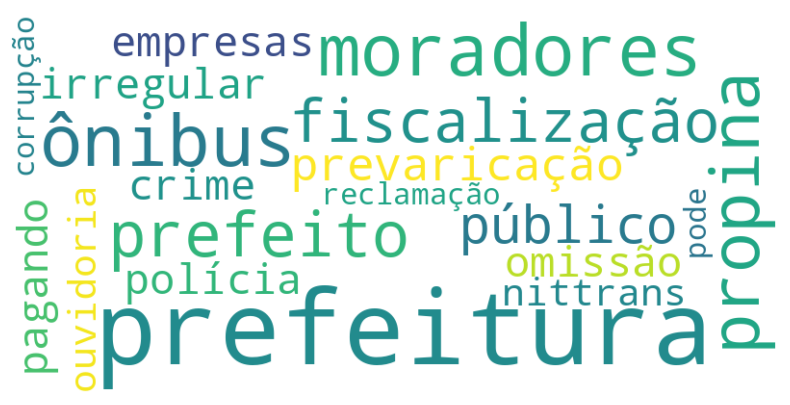
\includegraphics[width=0.7\textwidth]{images/wordcloud_corruption.png}
	\caption{Wordcloud com palavras mais frequentes em postagens sobre Corrupção}
	\label{fig:wordcloud_corruption}
\end{figure}

A polarização em torno desse tema é evidente, já que alguns usuários usam o Colab para denunciar casos de corrupção e exigir ação por parte das autoridades, enquanto outros podem discordar dessas alegações, defendendo que a corrupção não é a causa raiz dos problemas urbanos. Isso gera debates acalorados e uma atmosfera de pressão social em que diferentes opiniões colidem. Para compreender melhor como essa pressão social se manifesta, é fundamental analisar as métricas de score e persona em relação aos eventos urbanos.

A análise da pressão social nos eventos de zeladoria pública contém postagens que mencionam termos relacionados à corrupção, proporcionando uma visão profunda sobre como os usuários do Colab percebem essa questão em seu contexto urbano. O exame desses eventos revela a existência de uma polarização perceptível entre os usuários, refletida nas métricas de persona média e score médio. Entre os eventos, destaca-se o 'Ponto de infração de trânsito recorrente' com uma persona média de 1.0. indicando predominantemente o perfil \textit{complainer}. Isso sugere que os usuários estão recorrendo a essa categoria para denunciar e expressar insatisfação com infrações de trânsito recorrentes que podem ser atribuídas à corrupção no sistema de fiscalização.

Outro evento que chama a atenção é o 'Ponto recorrente de poluição sonora', também com uma persona média predominantemente \textit{complainer}. Nesse caso, os usuários estão relacionando a poluição sonora a possíveis atos corruptos que permitem a impunidade de estabelecimentos que desrespeitam as normas de emissão de ruídos. No entanto, alguns eventos surpreendem ao apresentar uma persona média \textit{complainer}, mas com scores médios positivos. Por exemplo, o 'Foco de mosquito da dengue/zika' e o 'Comércio aberto irregularmente' são eventos em que os usuários, embora manifestem preocupações relacionadas à corrupção, também demonstram uma inclinação para o perfil \textit{helper}. Isso sugere que, apesar das críticas à corrupção, os usuários estão dispostos a contribuir com soluções ou sugestões construtivas para lidar com esses problemas urbanos. Por outro lado, eventos como 'Bloqueio na via' e 'Via de terra com desnível' apresentam personas predominantemente \textit{complainer} com scores médios negativos, indicando uma alta insatisfação e falta de confiança nas autoridades em relação a essas questões. Os usuários parecem acreditar que a corrupção desempenha um papel significativo na má gestão da infraestrutura viária e na falta de manutenção adequada.

\begin{figure}[htb]
	\centering
	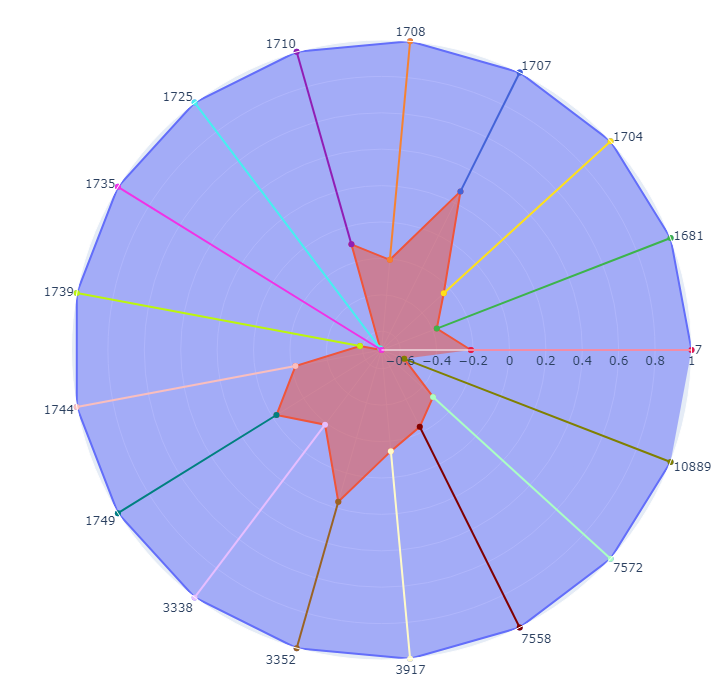
\includegraphics[width=0.7\textwidth]{images/social_barometer_corruption.png}
	\caption{Gráfico de Radar ilustrando a pressão social em relação ao tópico de Corrupção.}
	\label{fig:social_barometer_corruption}
\end{figure}

\begin{table}[htbp]
	\centering
	\caption{Métricas de pressão social do tópico de Corrupção}
	\label{tab:eventos_populares_corruption}
	\begin{tabular}{|l|c|c|c|c|}
		\hline
		\textbf{Tipo de Evento}                         & \textbf{Eventos} & \textbf{Score} & \textbf{Persona} \\
		\hline
		1681:Ponto recorrente de poluição sonora        & 4                & -0.3772        & 1.0000           \\
		\hline
		7:Ponto de infração de trânsito recorrente      & 3                & -0.2115        & 1.0000           \\
		\hline
		1707:Foco de mosquito da dengue/zika            & 2                & 0.2704         & 1.0000           \\
		\hline
		1708:Ponto de tráfico de drogas                 & 2                & -0.2053        & 1.0000           \\
		\hline
		7558:Ocupação irregular de área pública         & 2                & -0.2315        & 1.0000           \\
		\hline
		3352:Comércio aberto irregularmente             & 2                & 0.1643         & 1.0000           \\
		\hline
		1749:Manutenção de semáforo                     & 1                & -0.0244        & 1.0000           \\
		\hline
		7572:Estabelecimento sem nota fiscal            & 1                & -0.3197        & 1.0000           \\
		\hline
		3917:Calçada irregular                          & 1                & -0.1449        & 1.0000           \\
		\hline
		3338:Iluminação pública irregular               & 1                & -0.1885        & 1.0000           \\
		\hline
		1739:Evento Irregular                           & 1                & -0.5827        & 1.0000           \\
		\hline
		1744:Ônibus danificado                          & 1                & -0.2220        & 1.0000           \\
		\hline
		1735:Via de terra com desnível                  & 1                & -0.7028        & 1.0000           \\
		\hline
		1725:Bloqueio na via                            & 1                & -0.6911        & 1.0000           \\
		\hline
		1710:Ponto de assalto/roubo                     & 1                & -0.0995        & 1.0000           \\
		\hline
		1704:Calçada inexistente                        & 1                & -0.2403        & 1.0000           \\
		\hline
		10889:Placa de sinalização quebrada/inexistente & 1                & -0.5688        & 1.0000           \\
		\hline
	\end{tabular}
\end{table}

Em síntese, a análise dos eventos relacionados à corrupção evidencia uma dinâmica complexa de pressão social no Colab. Embora os usuários manifestem insatisfação e preocupação com a corrupção em diversas esferas da administração pública, a polarização entre os perfis \textit{complainer} e \textit{helper} se destaca de forma clara. Alguns eventos refletem uma abordagem mais equilibrada, na qual os usuários não se limitam a críticas, mas também se empenham na busca por soluções construtivas. Esses resultados sublinham a importância de adotar uma abordagem abrangente para enfrentar a corrupção e os desafios urbanos, engajando os cidadãos de maneira mais eficaz e fomentando a transparência e a responsabilidade governamental.

\subsection{Eleições e Políticos}

As discussões sobre eleições e políticos no contexto dos problemas urbanos no Brasil são um reflexo evidente da interseção entre a política e as questões que afetam diretamente a vida dos cidadãos. No Colab, plataforma dedicada a identificar e solucionar problemas nas cidades, os usuários frequentemente abordam não apenas as questões relacionadas à infraestrutura e serviços públicos, mas também fazem conexões intrincadas com o cenário político do país. Essa dinâmica cria um ambiente propício para debates acalorados e polarização de opiniões.

Assim como muitos cidadãos expressam sua insatisfação com impostos elevados e tarifas onerosas, eles também utilizam o Colab como um espaço para relacionar os problemas urbanos às promessas e ações de políticos, além de destacar a ineficiência e as questões políticas subjacentes. É aqui que a polarização se manifesta de forma mais clara, com alguns usuários apoiando determinados políticos e partidos, enquanto outros discordam veementemente. Essa polarização não apenas reflete as divisões políticas na sociedade brasileira, mas também contribui para uma discussão intensa e muitas vezes apaixonada sobre como a política impacta diretamente a qualidade de vida nas cidades.

\begin{figure}[htb]
	\centering
	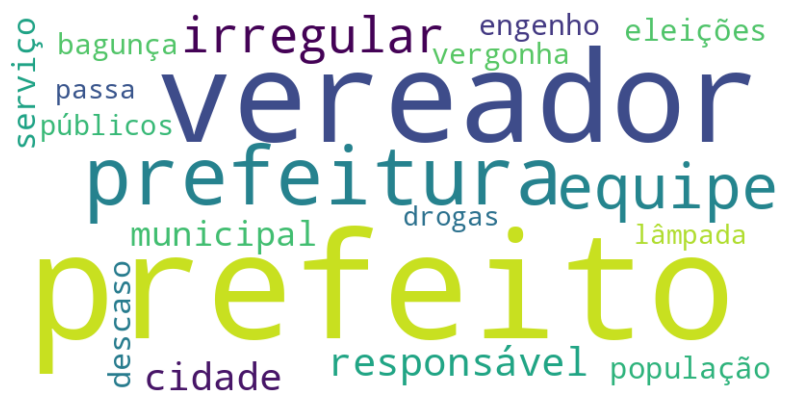
\includegraphics[width=0.7\textwidth]{images/wordcloud_polititians.png}
	\caption{Wordcloud com palavras mais frequentes em postagens sobre Eleições e Políticos}
	\label{fig:wordcloud_polititians}
\end{figure}

Os usuários frequentemente mencionam políticos de diferentes partidos, como PT, PDT, PSDB e PSOL, refletindo a diversidade política da cidade. As discussões em torno de políticos e partidos podem ser calorosas e refletem a interseção entre política e questões urbanas, como infraestrutura e serviços públicos. Durante períodos eleitorais, como as eleições para prefeito e vereador, a pressão social em torno desse tópico aumenta significativamente. Os eleitores discutem candidatos, suas propostas e o histórico de mandatos anteriores. Eles também compartilham informações sobre como registrar seus votos, destacando a importância da participação cívica. A pressão social relacionada a políticos e eleições é frequentemente acompanhada de debates sobre o desempenho dos vereadores e prefeitos atuais. Os cidadãos avaliam seus mandatos, destacando conquistas e críticas. A palavra 'vereador' é mencionada com frequência, sugerindo que a atuação desses representantes municipais é uma preocupação central para os cidadãos.

É interessante notar que, entre todas as siglas de partidos políticos pesquisadas, a única que aparece com sentimentos consideravelmente negativos é o PT (Partido dos Trabalhadores). Isso pode indicar que os usuários associam o PT a problemas específicos na cidade, resultando em sentimentos negativos. Essa associação pode ser influenciada por eventos passados ou pela percepção da atuação do partido.

A análise da pressão social relacionada ao tópico revela uma dinâmica complexa e polarizada. Para compreender melhor essas dinâmicas, é essencial considerar tanto o score médio de sentimento quanto a persona média atribuída aos usuários em relação a tipos específicos de eventos de zeladoria pública. Primeiramente, ao observarmos os eventos selecionados, podemos identificar uma variação significativa nos valores médios de score de sentimento e persona média. Alguns eventos apresentam uma persona média predominantemente \textit{helper}, indicando que os usuários tendem a adotar uma postura mais positiva e colaborativa em relação a esses eventos. Por outro lado, há eventos em que a persona média é predominantemente \textit{complainer}, sinalizando uma postura mais crítica e insatisfeita dos usuários.

\begin{figure}[htb]
	\centering
	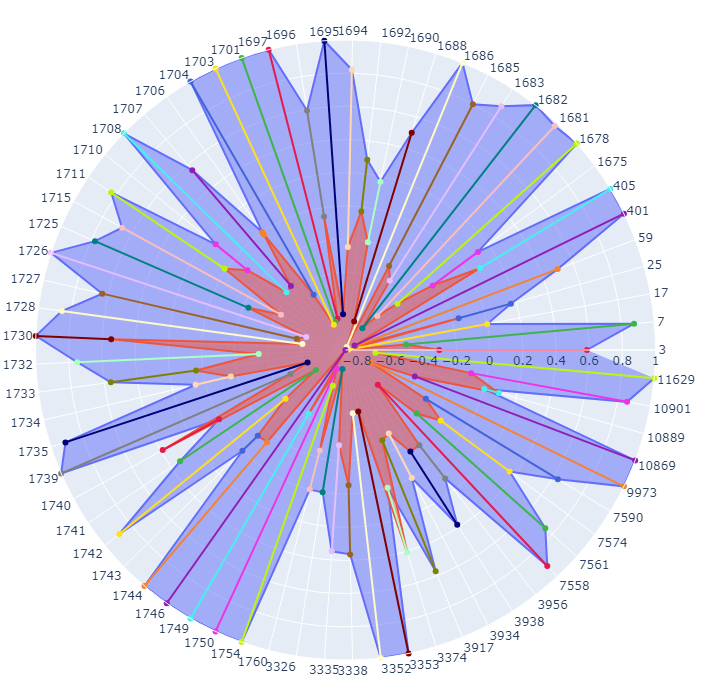
\includegraphics[width=0.7\textwidth]{images/social_barometer_polititians.png}
	\caption{Gráfico de Radar ilustrando a pressão social em relação ao tópico de Eleições e Políticos.}
	\label{fig:social_barometer_polititians}
\end{figure}

\begin{table}[htbp]
	\centering
	\caption{Métricas de pressão social do tópico de Eleições e Políticos.}
	\label{tab:eventos_populares_polititians}
	\begin{tabular}{|l|c|c|c|c|}
		\hline
		\textbf{Tipo de Evento}                         & \textbf{Eventos} & \textbf{Score} & \textbf{Persona} \\
		\hline
		1681:Ponto recorrente de poluição sonora        & 4                & -0.3772        & 1.0000           \\
		\hline
		7:Ponto de infração de trânsito recorrente      & 3                & -0.2115        & 1.0000           \\
		\hline
		1707:Foco de mosquito da dengue/zika            & 2                & 0.2704         & 1.0000           \\
		\hline
		1708:Ponto de tráfico de drogas                 & 2                & -0.2053        & 1.0000           \\
		\hline
		7558:Ocupação irregular de área pública         & 2                & -0.2315        & 1.0000           \\
		\hline
		3352:Comércio aberto irregularmente             & 2                & 0.1643         & 1.0000           \\
		\hline
		1749:Manutenção de semáforo                     & 1                & -0.0244        & 1.0000           \\
		\hline
		7572:Estabelecimento sem nota fiscal            & 1                & -0.3197        & 1.0000           \\
		\hline
		3917:Calçada irregular                          & 1                & -0.1449        & 1.0000           \\
		\hline
		3338:Iluminação pública irregular               & 1                & -0.1885        & 1.0000           \\
		\hline
		1739:Evento Irregular                           & 1                & -0.5827        & 1.0000           \\
		\hline
		1744:Ônibus danificado                          & 1                & -0.2220        & 1.0000           \\
		\hline
		1735:Via de terra com desnível                  & 1                & -0.7028        & 1.0000           \\
		\hline
		1725:Bloqueio na via                            & 1                & -0.6911        & 1.0000           \\
		\hline
		1710:Ponto de assalto/roubo                     & 1                & -0.0995        & 1.0000           \\
		\hline
		1704:Calçada inexistente                        & 1                & -0.2403        & 1.0000           \\
		\hline
		10889:Placa de sinalização quebrada/inexistente & 1                & -0.5688        & 1.0000           \\
		\hline
	\end{tabular}
\end{table}

Um exemplo de evento com persona predominantemente \textit{helper} é o tipo 'Limpeza de área pública' indicando uma atitude positiva e colaborativa dos usuários em relação à limpeza de áreas públicas. O score médio de sentimento é majoritariamente negativo, mas a persona média positiva sugere que os usuários, apesar das críticas, estão dispostos a contribuir para soluções construtivas. Nesse caso, o sentimento prendominante parece ser de cobrar os políticos pelo voto de confiança de seus eleitores e oferecer críticas mais construtivas. Por outro lado, o evento 'Calçada inexistente' apresenta uma persona média de 1.0. indicando uma postura crítica e insatisfeita dos usuários em relação à falta de calçadas. O score médio de sentimento é de -0.484, corroborando o sentimento negativo. Nesse caso, os usuários parecem expressar insatisfação e não demonstram uma postura colaborativa em relação à questão das calçadas.

A polarização se torna evidente ao analisar eventos como 'Ponto de infração de trânsito recorrente', que possui uma persona média de 0.878, indicando uma postura crítica e insatisfeita, juntamente com um score médio de sentimento de -0.501, refletindo um sentimento negativo. Nesse contexto, os usuários estão claramente insatisfeitos com a infração de trânsito recorrente e expressam críticas contundentes. Esse tipo de evento especifico parece gerar uma postura mais crítica dos usuários em vários tópicos de pressão social diferentes.

Esses resultados demonstram que os usuários do Colab têm uma postura diversificada em relação aos problemas urbanos, algumas vezes relacionando ao período eleitoral e as motivações dos políticos. Alguns eventos atraem uma postura mais colaborativa, enquanto outros geram críticas intensas e insatisfação. Isso sugere que a polarização é uma característica proeminente dessas discussões, com alguns usuários apoiando políticos e partidos específicos, enquanto outros expressam descontentamento. Além disso, a análise das métricas de pressão social revela que a qualidade da infraestrutura urbana e os problemas relacionados à gestão pública são temas de grande relevância para os cidadãos. A frequente menção de políticos, partidos e eleições nas postagens dos usuários indica que a política tem um impacto significativo na percepção dos problemas urbanos. Durante períodos eleitorais, a pressão social aumenta, com discussões detalhadas sobre candidatos, propostas e desempenho de representantes eleitos.

Em resumo, a análise dos eventos relacionados à percepção dos usuários sobre 'Eleições e Políticos' destaca a complexidade das interações sociais e das atitudes dos usuários em relação aos problemas urbanos. Embora exista uma insatisfação geral com a eficiência dos políticos, a predominância de personas \textit{helper} sugere que os usuários estão dispostos a colaborar ativamente na solução desses problemas, demonstrando uma vontade de participar ativamente na busca por soluções. Por outro lado, a associação negativa com determinadas vertentes políticas indica que as percepções políticas também desempenham um papel importante nas discussões sobre pressão social e problemas urbanos, influenciando a forma como os usuários abordam e debatem essas questões. Portanto, a polarização política e a complexidade das interações sociais são aspectos essenciais a serem considerados ao abordar a dinâmica das discussões sobre problemas urbanos e políticos, exigindo uma abordagem equilibrada e inclusiva na busca por soluções eficazes.

\section{Mapeando a Opinião Pública}

O experimento de análise das discussões no Colab nos trouxe valiosos insights sobre a diversidade de perspectivas e abordagens dos usuários em relação a uma variedade de tópicos urbanos. Ao examinar os valores de persona média e score médio em eventos relacionados a pressão social, como paisagismo, meio ambiente, gentrificação, higienismo social, segurança pública, drogas, pânico moral, política tributária, corrupção e políticos, pudemos identificar tendências interessantes que lançam luz sobre a dinâmica das discussões na plataforma.

Primeiramente, ficou evidente que não existe um único tipo de evento com uma persona predominante \textit{helper} ou \textit{complainer}. A distribuição de personas e scores varia amplamente entre os eventos, refletindo a complexidade e a diversidade das questões urbanas. Isso nos leva a concluir que a comunidade do Colab aborda diferentes problemas com uma ampla gama de atitudes, desde a busca ativa por soluções até a expressão de críticas construtivas ou negativas.

Além disso, a análise revelou que mesmo nas discussões em que predominam as personas \textit{helper} ainda podem surgir críticas construtivas, e nas discussões com predominância de personas \textit{complainer} ainda podem existir elementos construtivos. Isso sugere que os usuários estão dispostos a considerar diferentes perspectivas e contribuir para melhorias, independentemente de sua atitude inicial em relação ao problema.

Quanto à polarização no Colab, observamos que, embora as discussões possam ser críticas e até mesmo negativas em alguns casos, a maioria dos usuários parece estar comprometida em abordar e resolver os desafios urbanos. A polarização pode estar presente em debates políticos e em tópicos sensíveis, como corrupção e gentrificação, mas a presença significativa de personas \textit{helper} indica uma disposição para encontrar soluções construtivas, mesmo em meio a divergências.

\begin{figure}[htb]
	\centering
	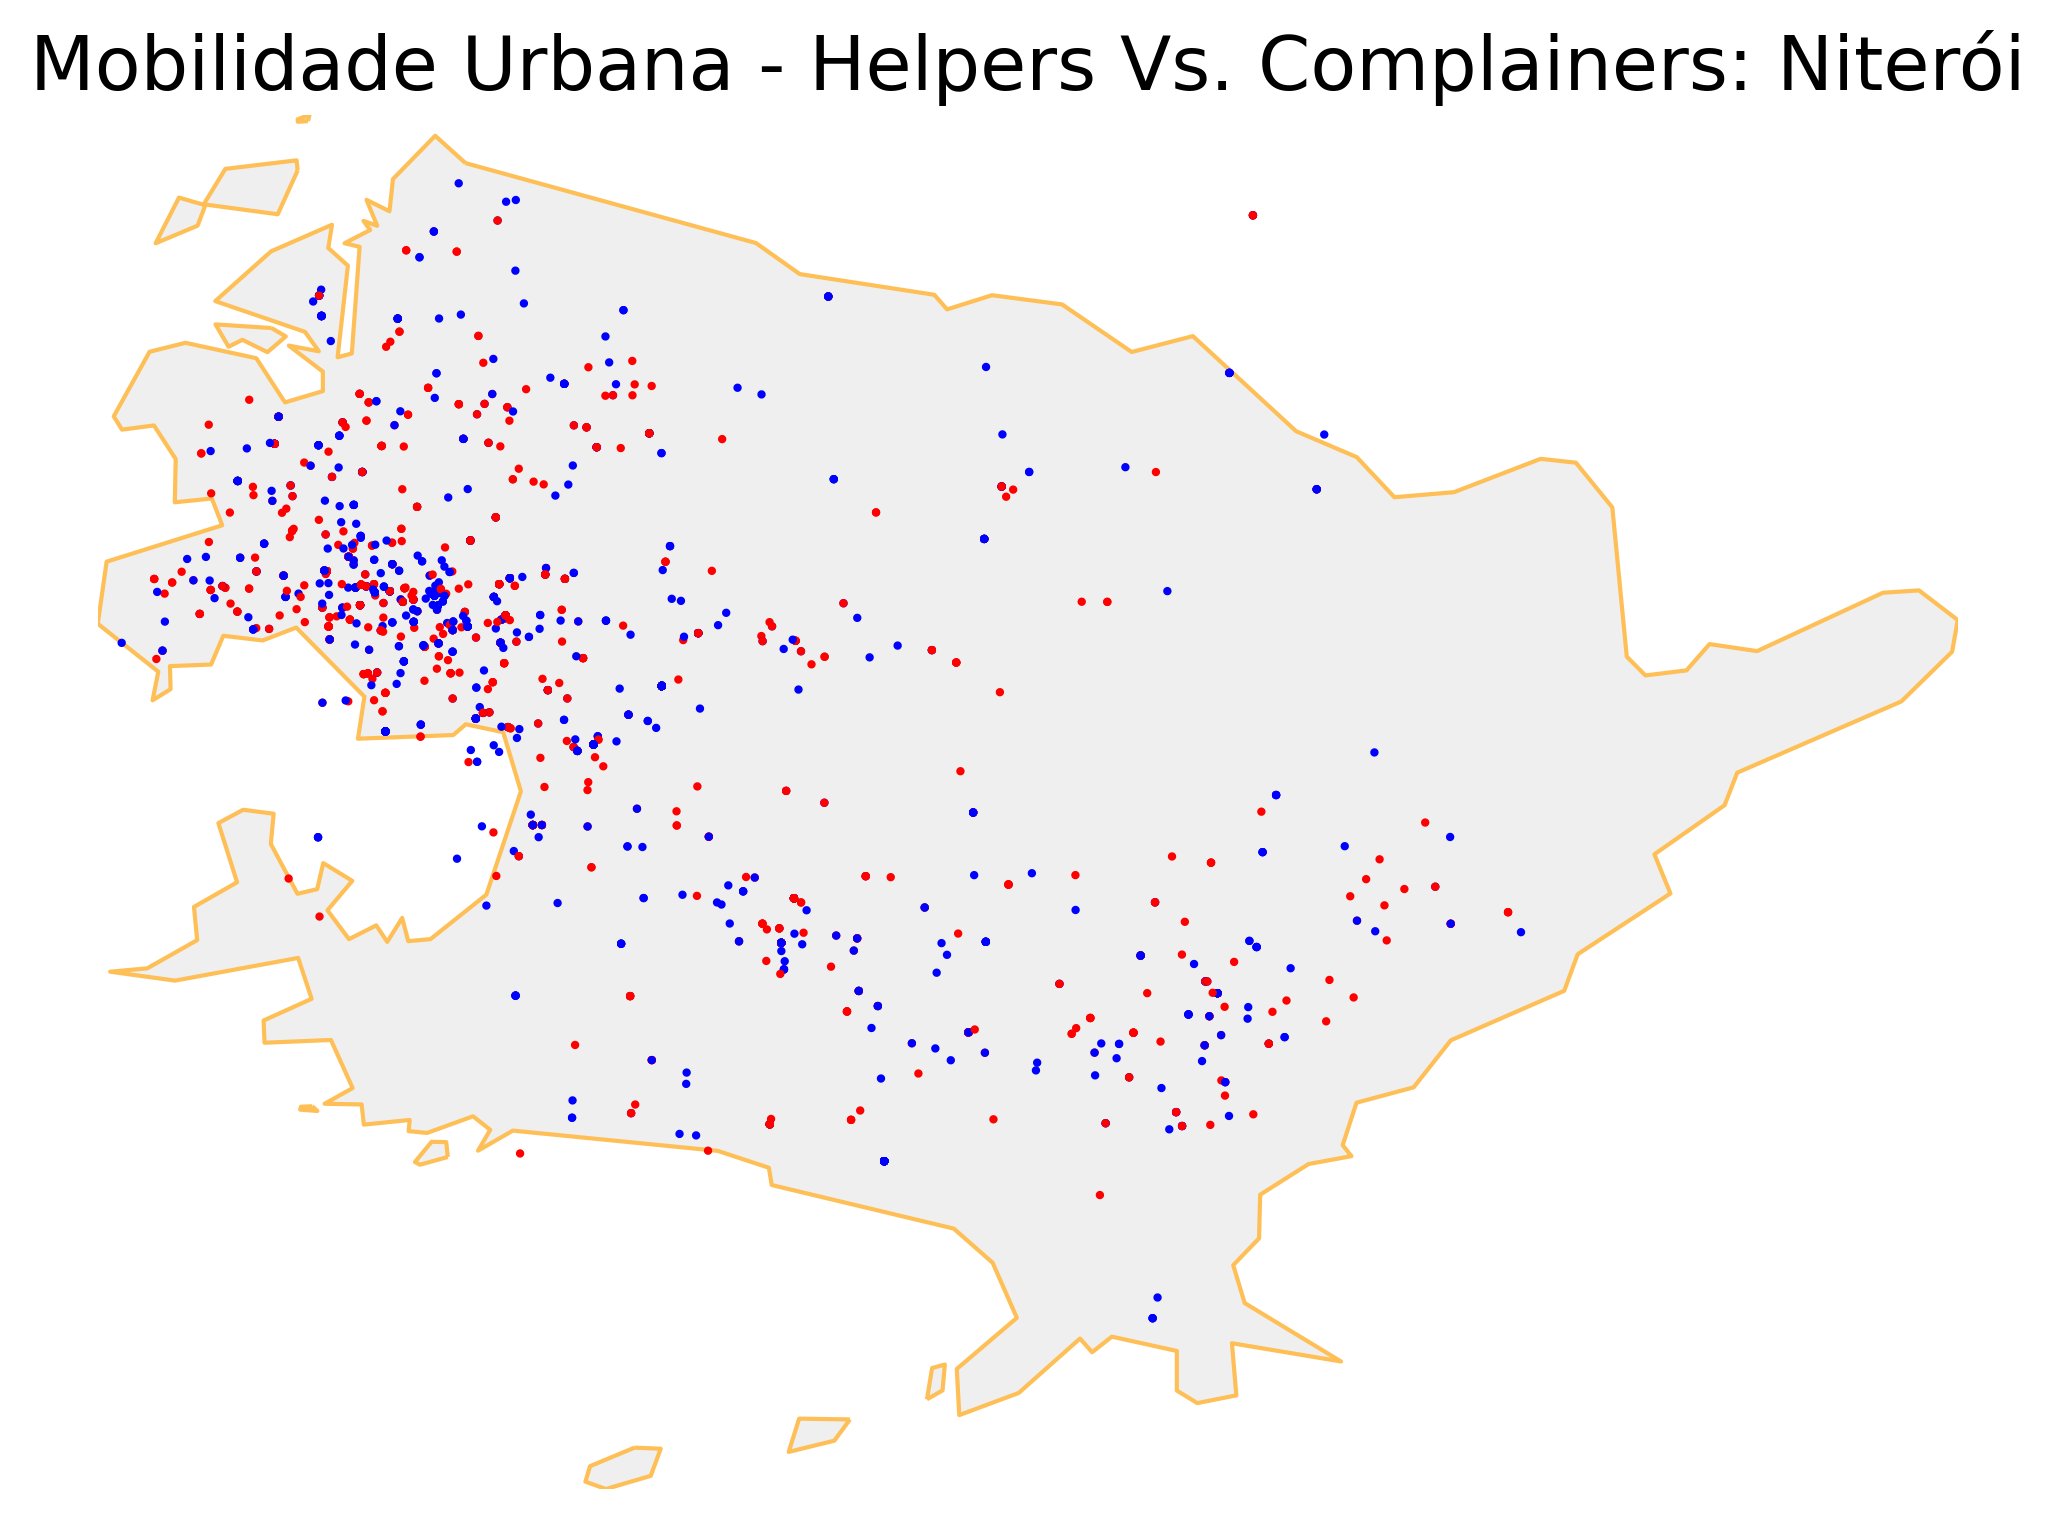
\includegraphics[width=0.7\textwidth]{images/network_niteroi_personas_plot.png}
	\caption{Mobilidade Urbana - Helpers vs. Complainers em Niterói.}
	\label{fig:network_niteroi_personas_plot}
\end{figure}

É interessante observar como uma abordagem de engenharia de software pode ser aplicada a um problema social complexo como a análise de pressão social hiperlocal no Colab. As heurísticas desenvolvidas no início do capítulo desempenham um papel crucial na criação de métricas quantitativas que permitem medir a opinião média e as personas dos usuários em relação a diferentes tipos de eventos de zeladoria pública. Além disso, essas heurísticas fornecem uma base sólida para a criação de representações visuais, como o gráfico de radar, que ajudam a visualizar as dinâmicas sociais de forma acessível.

A coleta de dados estruturados, através do desenvolvimento de um modelo de dados bem definido, é essencial para organizar informações relevantes, proporcionando uma compreensão clara dos elementos essenciais para a análise. Além disso, a aplicação de algoritmos de classificação e processamento de linguagem natural, como o uso de aprendizado de máquina para classificar usuários em personas e atribuir scores de sentimento às postagens, automatiza análises complexas de texto, economizando tempo e recursos.

A criação de representações visuais, como o gráfico de radar, desempenha um papel crucial na comunicação de insights complexos de maneira acessível. Essas visualizações destacam padrões e tendências, facilitando a tomada de decisões informadas. A abordagem de engenharia de software também permite a iteração e o aprendizado contínuo, possibilitando melhorias constantes no sistema com base em resultados e em evoluções nas dinâmicas sociais.

A integração eficaz das análises e insights com os tomadores de decisão, como agências governamentais e organizações da sociedade civil, é fundamental para garantir que os resultados sejam aplicados para informar políticas e ações práticas. Essa abordagem colaborativa promove uma governança mais informada e eficaz, aproveitando a tecnologia para compreender e resolver problemas sociais complexos.

A aplicação de abordagens de engenharia de software à análise de problemas sociais complexos é uma maneira eficaz de aproveitar a tecnologia para compreender melhor as dinâmicas sociais, identificar áreas de preocupação e promover o envolvimento cidadão. Além disso, a abordagem iterativa permite que o sistema evolua e se adapte às necessidades em constante mudança das comunidades urbanas, contribuindo para uma governança mais informada e eficaz.

O experimento nos ensinou que a plataforma Colab é um reflexo da complexidade das questões urbanas e das opiniões diversificadas de seus usuários. Podemos aprender que a diversidade de perspectivas é uma força, pois permite a consideração de uma ampla gama de soluções para os problemas urbanos. A análise também nos lembra da importância de um diálogo construtivo e da busca de soluções colaborativas para promover uma cidade mais eficiente, segura e inclusiva.

Em um mundo onde as divisões são cada vez mais comuns, o Colab nos mostra que, apesar das diferenças, as comunidades podem se unir em busca de um objetivo comum: tornar as cidades melhores lugares para se viver. Portanto, ao continuar a incentivar o diálogo e a colaboração, o Colab pode desempenhar um papel importante na melhoria das condições urbanas e na promoção do bem-estar de todos os cidadãos.

\section{Aspectos hiperlocais}

Ao explorarmos a dinâmica da pressão social e sua manifestação por meio de discussões e relatos de problemas urbanos no Colab, entendemos como os usuários da plataforma expressam preocupações, sentimentos e opiniões sobre uma variedade de tópicos, destacando as questões mais relevantes e polarizadoras que afetam suas comunidades. Agora, avançaremos na análise para ressaltar o aspecto hiperlocal, concentrando-nos na comparação entre as três cidades analisadas.

No âmbito da pressão social hiperlocal, é essencial reconhecer que diferentes localidades podem reagir de maneiras diversas aos mesmos problemas urbanos. Niterói e Mesquita, situadas no estado do Rio de Janeiro, e Santo André, localizada em São Paulo, compartilham desafios comuns enfrentados por muitas cidades brasileiras, como infraestrutura, segurança pública e qualidade de vida. No entanto, a percepção e a priorização desses desafios podem variar significativamente entre essas duas cidades.

Para entender melhor essas nuances, analisamos os tipos de eventos mais criados em Niterói, Mesquita e Santo André. Embora ambos os municípios enfrentem problemas relacionados a buracos nas vias e lâmpadas apagadas à noite, a classificação dos tipos de eventos revela diferenças marcantes. Niterói apresenta uma alta incidência de eventos relacionados a problemas nas vias, como 'Buraco nas vias' 'Calçada irregular' e 'Ponto de infração de trânsito recorrente'. Esses eventos estão diretamente ligados à mobilidade urbana e à infraestrutura viária, indicando uma preocupação significativa dos cidadãos em relação a essa questão. Portanto, um tópico de pressão social relevante para Niterói é a 'Mobilidade Urbana'. Mesquita tem um grande número de eventos relacionados à natureza e ao meio ambiente, como 'Poda de árvore' e 'Mato alto'. Esses eventos indicam uma preocupação com a preservação ambiental e o paisagismo urbano. Portanto, um tópico de pressão social relevante para Santo André é o 'Meio Ambiente'. Santo André enfrenta desafios relacionados à limpeza e à infraestrutura urbana, como 'Entulho na calçada/via pública' e 'Esgoto a céu aberto'. Esses problemas podem afetar diretamente a saúde pública dos cidadãos. Portanto, um tópico de pressão social relevante para Santo André é a 'Saúde Pública'.

Embora esses tópicos sejam relevantes para as três cidades, a análise revela que cada uma delas tem uma percepção e uma priorização únicas dos problemas urbanos. Essas diferenças podem ser atribuídas a uma variedade de fatores, como a infraestrutura urbana, a composição demográfica e a cultura local. A análise também destaca a importância de uma abordagem hiperlocal para entender melhor as necessidades e os desafios de cada comunidade. Ao considerar essas nuances, os gestores públicos podem tomar decisões mais informadas e eficazes, contribuindo para uma governança mais inclusiva e participativa. Essa análise inicial destaca como as diferentes cidades reagem e percebem os problemas urbanos de maneira única, mesmo quando enfrentam desafios semelhantes. A partir desses dados, podemos aprofundar nossa investigação para entender melhor os fatores locais que moldam essas percepções e prioridades, contribuindo para uma compreensão mais abrangente da pressão social hiperlocal e suas implicações na gestão urbana.

A partir da definição dos tópicos a serem analisados, desenvolvemos uma metodologia para criar visualizações de pressão social hiperlocal utilizando dados de geolocalização de eventos postados em mídias sociais. A metodologia emprega bibliotecas como Folium e Bokeh para a geração dos mapas interativos e gráficos de rede. Primeiramente, os dados são filtrados para uma região de interesse, no caso, a cidade de Santo André. Em seguida, são selecionadas palavras-chave relevantes relacionadas à saúde pública, tais como 'hospital' 'pronto socorro' 'vacinação' entre outras. Eventos que não estão diretamente relacionados a essas palavras-chave são excluídos do conjunto de dados. A visualização inclui dois componentes principais: mapas de calor (heatmaps) e um gráfico de rede (network).

Para os heatmaps, a ponderação é ajustada com base em uma métrica de sentimento, e um mapa base é criado, centrado na média das coordenadas geográficas dos eventos selecionados. Os dados ponderados são utilizados para gerar o mapa de calor, com uma escala de cores que indica o sentimento dos eventos.

No gráfico de rede, as conexões entre os eventos e os usuários que os postaram são identificadas e representadas. A biblioteca NetworkX é utilizada para criar o gráfico, e os nós são posicionados com base nas coordenadas geográficas dos eventos. Uma adição importante à visualização é a coloração dos nós com base nas personas identificadas: azul para os \textit{helpers}  e vermelho para os \textit{complainers}. Além disso, o polígono da cidade é utilizado como referência para centralizar tanto o mapa de rede quanto os pontos de eventos. Isso contribui significativamente para destacar a localização dos eventos em relação à área geográfica da cidade, possibilitando uma análise mais detalhada das dinâmicas de saúde pública em nível hiperlocal.

Essas visualizações permitem a identificação de padrões de atividade relacionados aos tópicos de pressão social a nível hiperlocal. Os heatmaps revelam áreas de maior atividade e sentimentos associados aos eventos, permitindo uma compreensão mais granularizada das preocupações da comunidade em áreas específicas da cidade. O gráfico de rede, por sua vez, mostra como os eventos e usuários estão interconectados, possibilitando a identificação de influenciadores ou grupos de interesse em questões de saúde pública. A combinação de heatmaps e gráficos de rede fornece insights valiosos para formuladores de políticas públicas, pesquisadores e profissionais de saúde na tomada de decisões e no planejamento de intervenções em saúde pública a nível hiperlocal.

\subsection{Mobilidade Urbana em Niterói}

A análise dos resultados de pressão social relacionados à mobilidade urbana em Niterói revela uma série de insights sobre as preocupações e percepções da comunidade em relação a esse tema crucial. Através da interpretação das métricas de 'Persona Média' e 'Score Médio', é possível discernir nuances nas atitudes dos cidadãos em relação a diferentes tipos de eventos.

\begin{figure}[htb]
	\centering
	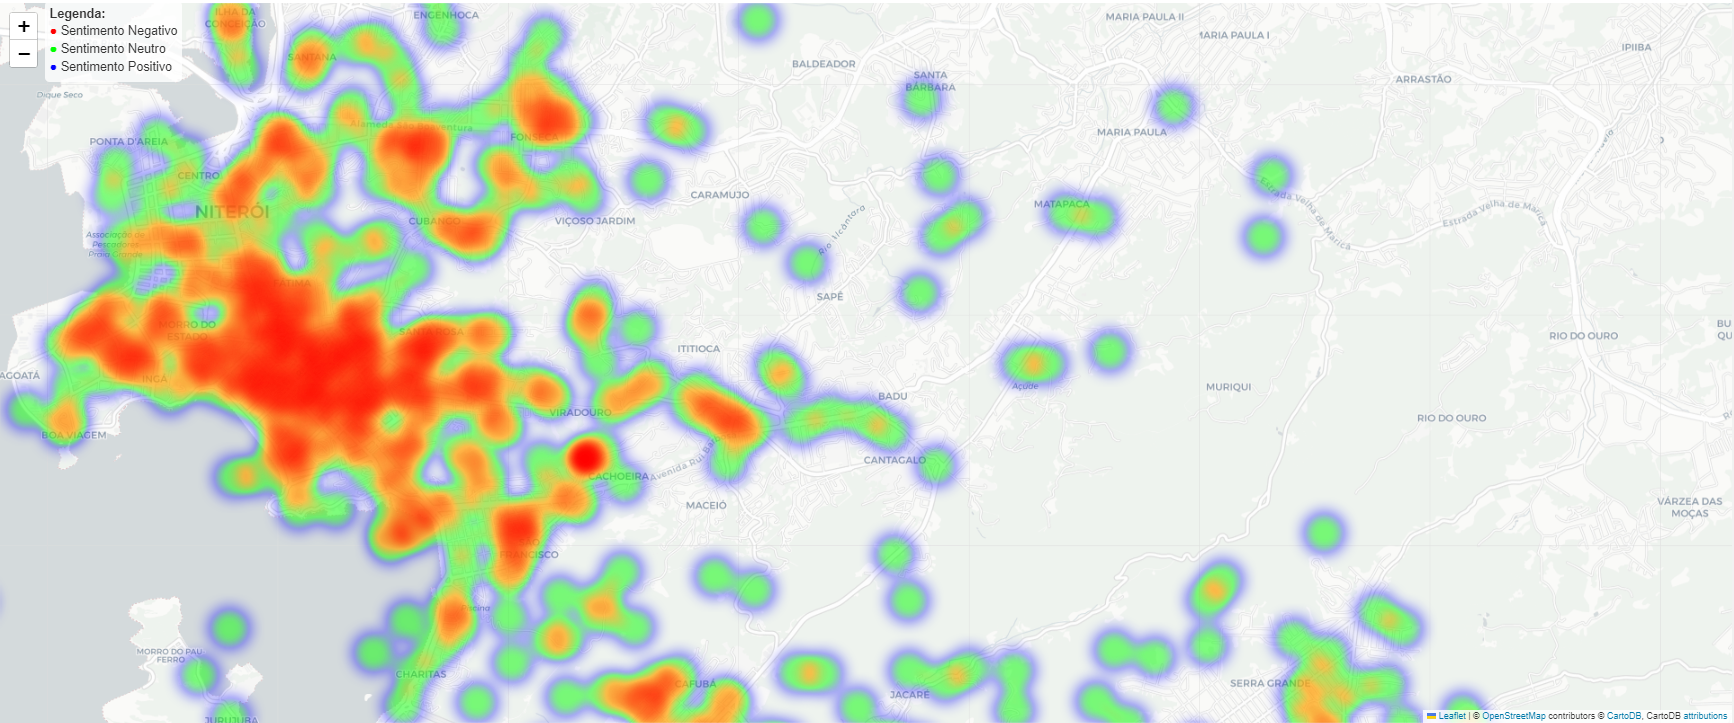
\includegraphics[width=0.7\textwidth]{images/heatmap_niteroi.PNG}
	\caption{Heatmap de Pressão Social para Mobilidade Urbana em Niterói}
	\label{fig:heatmap_niteroi}
\end{figure}

Primeiramente, é importante destacar a presença de eventos com uma persona média predominantemente \textit{complainer}. Isso sugere que há uma parcela da comunidade que expressa críticas e insatisfações em relação a certos aspectos da mobilidade urbana em Niterói. Um exemplo notável é o evento 'Estabelecimento com condição sanitária irregular', que apresenta uma persona média predominantemente \textit{complainer} e um score médio elevado. Isso indica que a comunidade está particularmente insatisfeita com a condição sanitária de alguns estabelecimentos na cidade, o que pode estar relacionado à mobilidade urbana, uma vez que essas condições podem afetar diretamente a experiência dos cidadãos ao utilizar os serviços públicos e privados.

Por outro lado, também existem eventos com uma persona média predominantemente \textit{helper}. Um exemplo é o evento 'Ponto de infração de trânsito recorrente', que possui uma persona média majoritariamente \textit{helper} e um score médio elevado. Isso sugere que, apesar das infrações de trânsito serem uma preocupação, a comunidade demonstra disposição para colaborar e apoiar a melhoria da situação, talvez através da denúncia dessas infrações e da promoção de um ambiente de trânsito mais seguro.

No que diz respeito aos eventos mais populares, 'Buraco nas vias' e 'Ponto de infração de trânsito recorrente' lideram a lista. Esses eventos estão intimamente ligados à infraestrutura viária e à segurança no trânsito, o que é consistente com as preocupações típicas de mobilidade urbana. A alta contagem de eventos nessas categorias reflete a importância dessas questões na mente dos cidadãos de Niterói, destacando a necessidade de investimentos e melhorias na malha viária da cidade.

Além disso, é relevante observar a presença de eventos relacionados à acessibilidade, como 'Rampa de acessibilidade irregular ou inexistente' e 'Estabelecimento com acessibilidade irregular'. Embora esses eventos também apresentem persona média predominantemente \textit{complainer}, eles apontam para desafios significativos em termos de acessibilidade na cidade, o que pode afetar diretamente a mobilidade de pessoas com deficiência e idosos. Isso ressalta a importância de políticas e ações que visem aprimorar a acessibilidade urbana.

\begin{figure}[htb]
	\centering
	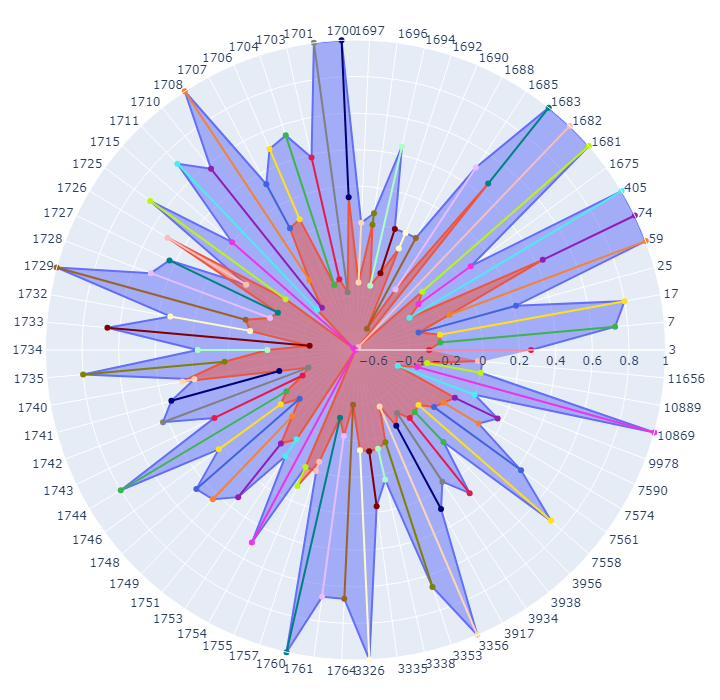
\includegraphics[width=0.7\textwidth]{images/social_barometer_niteroi.png}
	\caption{social barometer niteroi}
	\label{fig:social_barometer_niteroi}
\end{figure}

\begin{table}[htbp]
	\centering
	\caption{Pressão social do tópico Mobilidade Urbana em niteroi}
	\label{tab:eventos_populares_mobility_niteroi}
	\begin{tabular}{|l|c|c|c|c|}
		\hline
		\textbf{Tipo de Evento}                             & \textbf{Eventos} & \textbf{Score} & \textbf{Persona} \\
		\hline
		1725:Bloqueio na via                                & 15               & -0.2238        & 0.6919           \\
		\hline
		7:Ponto de infração de trânsito recorrente          & 15               & -0.2313        & 0.7299           \\
		\hline
		3:Buraco nas vias                                   & 13               & -0.2936        & 0.2642           \\
		\hline
		3938:Entulho na calçada/via pública                 & 12               & -0.2203        & 0.3056           \\
		\hline
		7561:Ponto de alagamento                            & 11               & -0.1653        & 0.4231           \\
		\hline
		7558:Ocupação irregular de área pública             & 11               & -0.2390        & 0.7246           \\
		\hline
		1727:Equipamento público danificado                 & 11               & -0.2255        & 0.4333           \\
		\hline
		1749:Manutenção de semáforo                         & 10               & -0.1963        & 0.4333           \\
		\hline
		3335:Lâmpada apagada à noite                        & 10               & -0.1376        & 0.1657           \\
		\hline
		1681:Ponto recorrente de poluição sonora            & 10               & -0.2128        & 1.0000           \\
		\hline
		3917:Calçada irregular                              & 9                & -0.2251        & 0.2913           \\
		\hline
		1741:Manutenção de ciclovia/ciclofaixa              & 9                & -0.2643        & 0.3487           \\
		\hline
		1704:Calçada inexistente                            & 8                & -0.3224        & 0.5385           \\
		\hline
		3338:Iluminação pública irregular                   & 7                & -0.1418        & 0.0323           \\
		\hline
		7574:Poda de árvore                                 & 7                & -0.1348        & 0.0882           \\
		\hline
		1746:Manutenção/implantação de placa de sinalização & 7                & -0.1914        & 0.2286           \\
		\hline
		1729:Ponto de transporte clandestino                & 7                & -0.0728        & 1.0000           \\
		\hline
		1703:Ponto de travessia irregular                   & 7                & -0.2995        & 0.3846           \\
		\hline
		1675:Bueiro sem tampa                               & 7                & -0.2707        & 0.0833           \\
		\hline
		25:Vazamento de água                                & 7                & -0.3388        & 0.2143           \\
		\hline
	\end{tabular}
\end{table}

Por fim, as métricas de pressão social também revelam eventos com sentimentos positivos e negativos. Por exemplo, eventos relacionados à poluição sonora e falta de energia tendem a ter uma persona média predominantemente \textit{complainer}, refletindo a insatisfação da comunidade com esses problemas. Por outro lado, eventos como 'Plantar uma árvore / Arborização' têm uma persona média predominantemente \textit{helper}, indicando um desejo de envolvimento na melhoria do ambiente urbano.

\begin{figure}[htb]
	\centering
	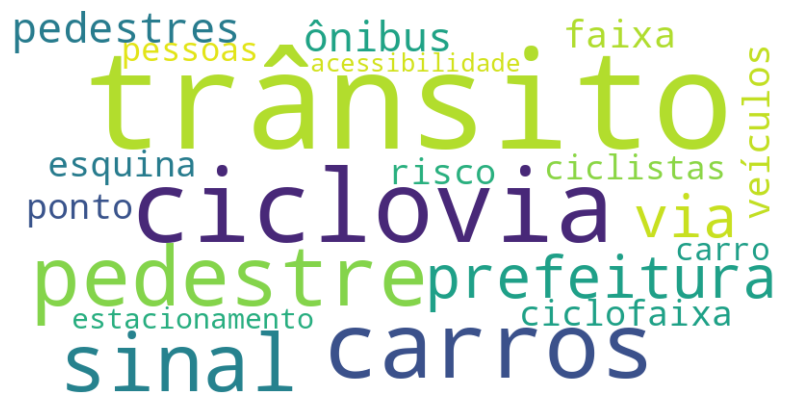
\includegraphics[width=0.7\textwidth]{images/wordcloud_niteroi.png}
	\caption{Palavras mais frequentes nas postagens de Niterói}
	\label{fig:wordcloud_niteroi}
\end{figure}

No contexto da malha urbana e viária de Niterói, esses resultados destacam a necessidade de um planejamento urbano abrangente que leve em consideração as preocupações e percepções da comunidade em relação à mobilidade. A presença de eventos com persona predominantemente \textit{complainer} em questões como infração de trânsito e condições sanitárias irregulares indica a importância de medidas de fiscalização e regulamentação para melhorar a segurança e a qualidade dos serviços urbanos. Por outro lado, a disposição da comunidade em denunciar infrações de trânsito sugere a necessidade de promover uma cultura de cumprimento das leis de trânsito.

\begin{figure}[htb]
	\centering
	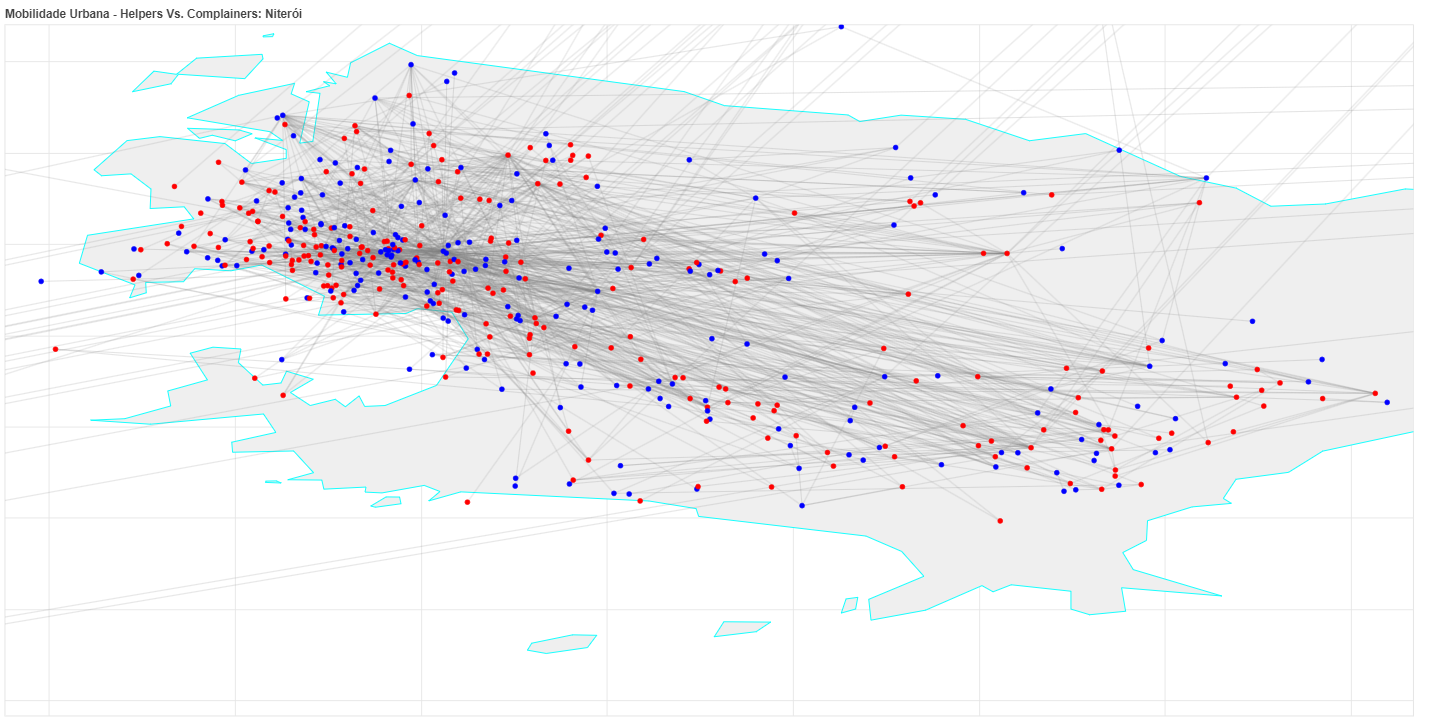
\includegraphics[width=0.7\textwidth]{images/network_niteroi_personas_map.png}
	\caption{Rede de eventos populares relacionados a mobilidade urbana em Niterói}
	\label{fig:network_niteroi_personas_map}
\end{figure}

Em relação à infraestrutura viária, a alta contagem de eventos relacionados a buracos nas vias aponta para a urgência de investimentos em manutenção e reparo da malha viária. Além disso, a presença de eventos relacionados à acessibilidade destaca a importância de tornar a cidade mais inclusiva para todos os cidadãos, incluindo pessoas com mobilidade reduzida.

Em resumo, as métricas de pressão social relacionadas à mobilidade urbana em Niterói oferecem uma visão valiosa das percepções e preocupações da comunidade. Esses insights podem ser utilizados pelas autoridades locais e organizações envolvidas na gestão urbana para direcionar seus esforços e políticas de maneira mais eficaz, promovendo uma mobilidade urbana mais segura, acessível e eficiente para todos os cidadãos.

\subsection{Meio Ambiente em Mesquita}
A análise dos resultados da pressão social relacionados ao tópico de meio ambiente em Mesquita revela uma série de insights importantes sobre as preocupações e percepções da comunidade local em relação a questões ambientais. Neste contexto, os eventos selecionados para análise incluem uma variedade de problemas ambientais, como descarte irregular de lixo, poluição do ar, desmatamento, entre outros. Através da interpretação das métricas de pressão social, é possível identificar tendências, polarizações e opiniões da comunidade em relação a esses problemas ambientais.

\begin{figure}[htb]
	\centering
	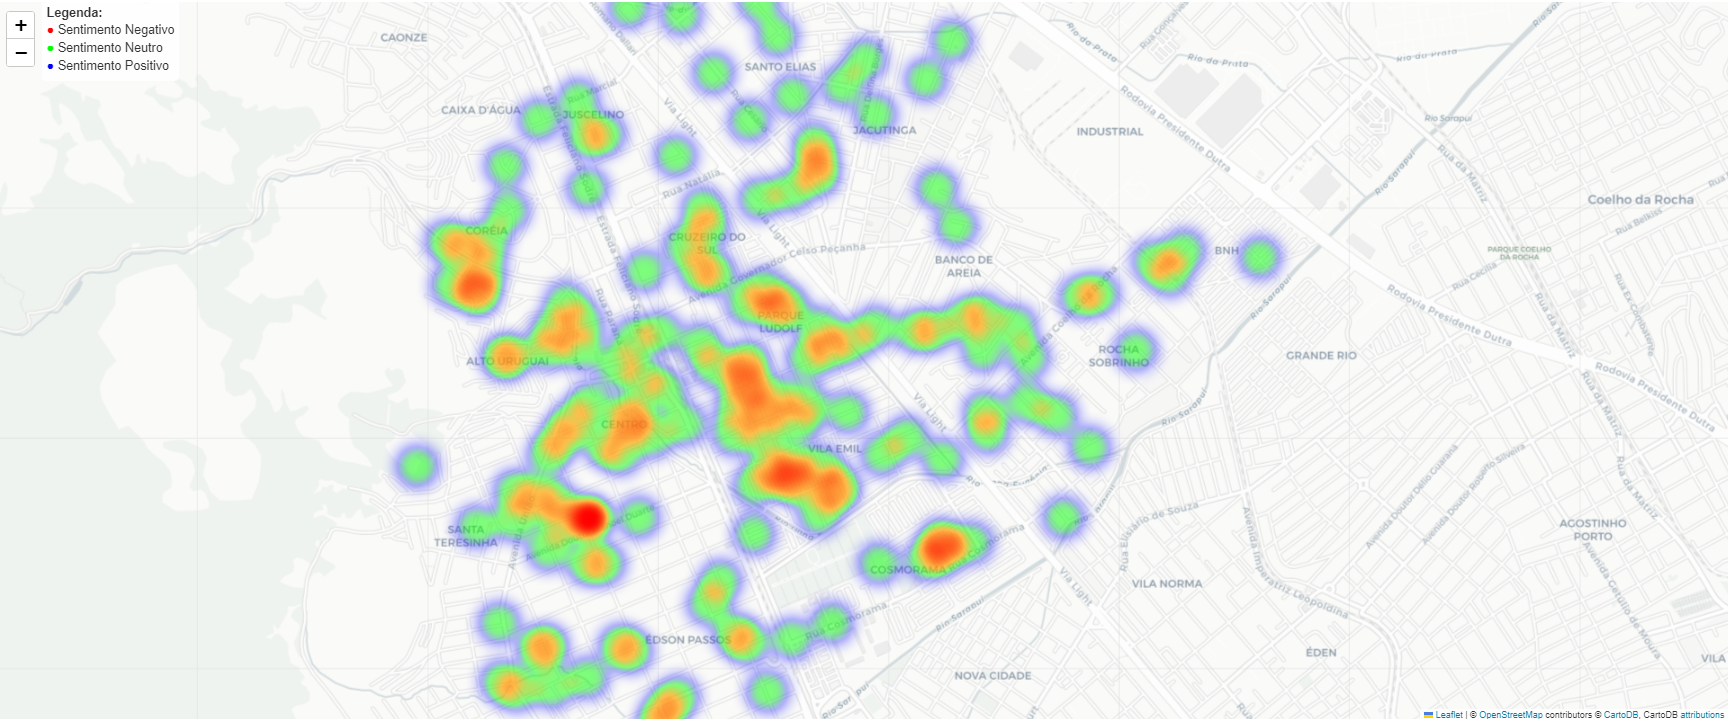
\includegraphics[width=0.7\textwidth]{images/heatmap_mesquita.PNG}
	\caption{Heatmap de Pressão Social para Meio Ambiente em Mesquita}
	\label{fig:heatmap_mesquita}
\end{figure}

Alguns eventos, como 'Descarte irregular de lixo' e 'Ponto de queimada irregular recorrente', apresentam uma persona média predominantemente \textit{complainer}, indicando que a comunidade está inclinada a relatar esses problemas com uma perspectiva crítica e negativa. Esses eventos também têm scores médios negativos, o que corrobora a percepção negativa em relação a esses problemas ambientais.

Por outro lado, eventos como 'Limpeza de Canais' e 'Poda de árvore' têm personas predominantemente \textit{helper} sugerindo que a comunidade está mais inclinada a relatar esses eventos de maneira positiva, possivelmente apoiando ações para a limpeza de canais e a poda de árvores. Esses eventos também têm scores médios positivos, refletindo uma visão mais favorável por parte da comunidade.

A análise dos eventos mais populares relacionados ao meio ambiente em Mesquita proporciona uma visão clara das principais preocupações da comunidade local. Dentre os eventos mais frequentes, destacam-se problemas como 'Descarte irregular de lixo' e 'Ponto de queimada irregular recorrente', ambos com uma persona média \textit{complainer} e scores médios negativos. Isso sugere que a questão do descarte inadequado de resíduos sólidos e a ocorrência de queimadas irregulares são fontes significativas de insatisfação e preocupação na comunidade.

\begin{figure}[htb]
	\centering
	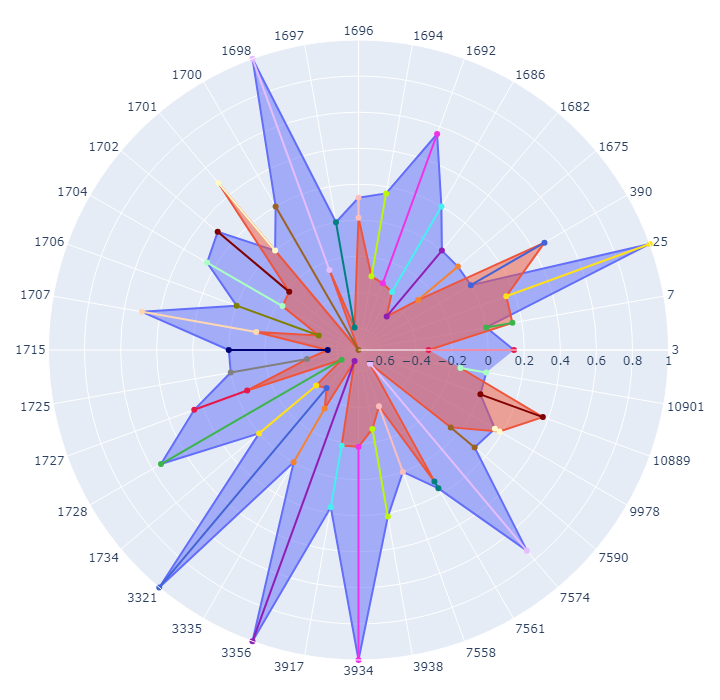
\includegraphics[width=0.7\textwidth]{images/social_barometer_mesquita.png}
	\caption{social barometer mesquita}
	\label{fig:social_barometer_mesquita}
\end{figure}

\begin{table}[htbp]
	\centering
	\caption{Pressão social do tópico Meio Ambiente em Mesquita}
	\label{tab:eventos_populares_mesquita}
	\begin{tabular}{|l|c|c|c|c|}
		\hline
		\textbf{Tipo de Evento}                         & \textbf{Eventos} & \textbf{Score} & \textbf{Persona} \\
		\hline
		3938:Entulho na calçada/via pública             & 5                & -0.2751        & 0.2188           \\
		\hline
		1700:Ponto de queimada irregular recorrente     & 5                & -0.7196        & 0.2000           \\
		\hline
		1694:Descarte irregular de lixo                 & 4                & -0.3045        & 0.1625           \\
		\hline
		1728:Imóvel ou terreno abandonado               & 4                & -0.6117        & 0.5455           \\
		\hline
		7590:Bueiro entupido                            & 3                & -0.0517        & 0.1212           \\
		\hline
		7574:Poda de árvore                             & 3                & -0.6205        & 0.7333           \\
		\hline
		1686:Emissão de fumaça preta                    & 3                & -0.3486        & 0.2000           \\
		\hline
		1696:Mato alto                                  & 3                & 0.0146         & 0.1250           \\
		\hline
		1727:Equipamento público danificado             & 2                & -0.0626        & 0.2500           \\
		\hline
		1704:Calçada inexistente                        & 2                & -0.2328        & 0.2500           \\
		\hline
		1702:Aterro sanitário irregular                 & 2                & -0.2180        & 0.3000           \\
		\hline
		3:Buraco nas vias                               & 2                & -0.3313        & 0.1429           \\
		\hline
		1734:Retirada de árvore                         & 2                & -0.4139        & 0.0000           \\
		\hline
		9978:Conservação (via pública)                  & 2                & 0.1833         & 0.1538           \\
		\hline
		10889:Placa de sinalização quebrada/inexistente & 1                & 0.3687         & 0.0000           \\
		\hline
		7558:Ocupação irregular de área pública         & 1                & -0.3874        & 0.0000           \\
		\hline
		3917:Calçada irregular                          & 1                & -0.1806        & 0.1667           \\
		\hline
		3356:Ônibus fora do horário/rota                & 1                & -0.6554        & 1.0000           \\
		\hline
		3335:Lâmpada apagada à noite                    & 1                & -0.3444        & 0.0000           \\
		\hline
		3321:Ponto recorrente de animais na via         & 1                & -0.4447        & 1.0000           \\
		\hline
	\end{tabular}
\end{table}

Outro evento frequente é 'Poda de árvore', que, como mencionado anteriormente, possui uma persona predominantemente \textit{helper} e um score médio positivo. Isso pode indicar que a comunidade valoriza e apoia ações de poda de árvores, possivelmente reconhecendo a importância da manutenção da vegetação urbana.

As métricas de pressão social relacionadas ao meio ambiente em Mesquita refletem a opinião da comunidade sobre questões ambientais. A presença de eventos com personas predominantemente \textit{complainer} e scores médios negativos indica que há preocupações significativas em relação ao meio ambiente na região. A negatividade nas avaliações sugere que muitos membros da comunidade estão insatisfeitos com a situação ambiental e estão relatando problemas de maneira crítica.

Por outro lado, a presença de eventos com personas predominantemente \textit{helper} e scores médios positivos demonstra que também há apoio e reconhecimento de esforços positivos relacionados ao meio ambiente. Isso sugere que parte da comunidade está engajada em ações de preservação ambiental e tem uma visão mais otimista em relação a essas questões.

As palavras-chave associadas aos eventos selecionados também oferecem insights sobre as preocupações da comunidade em relação ao meio ambiente. Palavras como 'descarte irregular de lixo' 'poluição' 'desmatamento' e 'queimadas' refletem as preocupações relacionadas à degradação ambiental, resíduos sólidos e degradação da vegetação.

\begin{figure}[htb]
	\centering
	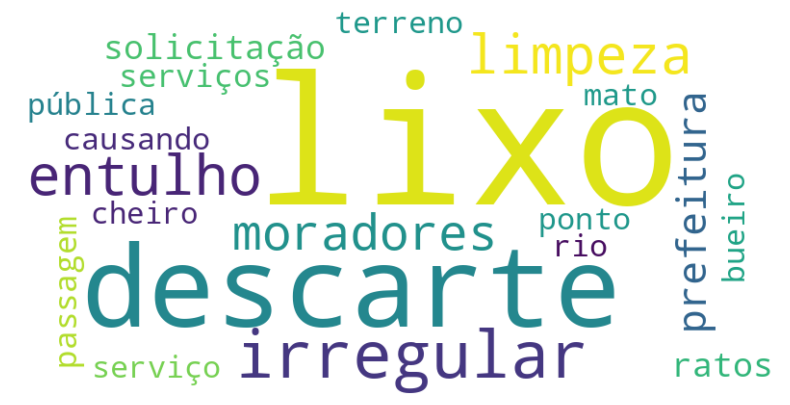
\includegraphics[width=0.7\textwidth]{images/wordcloud_mesquita.png}
	\caption{Wordcloud com palavras mais frequentes nas postagens de Mesquita}
	\label{fig:wordcloud_mesquita}
\end{figure}

É interessante notar que palavras como 'limpeza de canais' 'poda de árvore' e 'conservação (via pública)' também estão presentes, indicando que a comunidade reconhece a importância da limpeza de canais, manutenção de árvores e conservação da via pública como medidas positivas para proteger o meio ambiente.

A análise da pressão social relacionada ao meio ambiente em Mesquita revela uma diversidade notável de perspectivas e preocupações dentro da comunidade. Enquanto alguns eventos são relatados com uma perspectiva crítica e negativa, outros são percebidos de maneira mais otimista, refletindo uma clara polarização de opiniões.

As métricas de pressão social, incluindo persona média e score médio, oferecem uma visão abrangente das percepções da comunidade em relação a questões ambientais. Esses dados podem ser extremamente valiosos para as autoridades locais e organizações ambientais, uma vez que permitem direcionar de maneira mais eficaz seus esforços e políticas para abordar as preocupações específicas da comunidade.

Essa análise também ressalta a importância fundamental de envolver ativamente a comunidade na proteção e preservação ambiental. Reconhecer e responder às suas preocupações, promovendo ações direcionadas para melhorar a qualidade de vida e a sustentabilidade ambiental na região, torna-se uma prioridade evidente a partir dessas percepções variadas.

\subsection{Saúde Pública em Santo André}

A análise da pressão social relacionada à saúde pública em Santo André revela uma série de percepções e preocupações diversas na comunidade. Os eventos relatados abrangem uma ampla gama de questões, desde infraestrutura inadequada até problemas de higiene e segurança, refletindo a complexidade dessas preocupações. Ao examinarmos as métricas de pressão social podemos obter insights valiosos sobre como a comunidade percebe essas questões de saúde pública. É importante notar que essas métricas variam amplamente entre os diferentes tipos de eventos, indicando uma diversidade de opiniões e sentimentos.

\begin{figure}[htb]
	\centering
	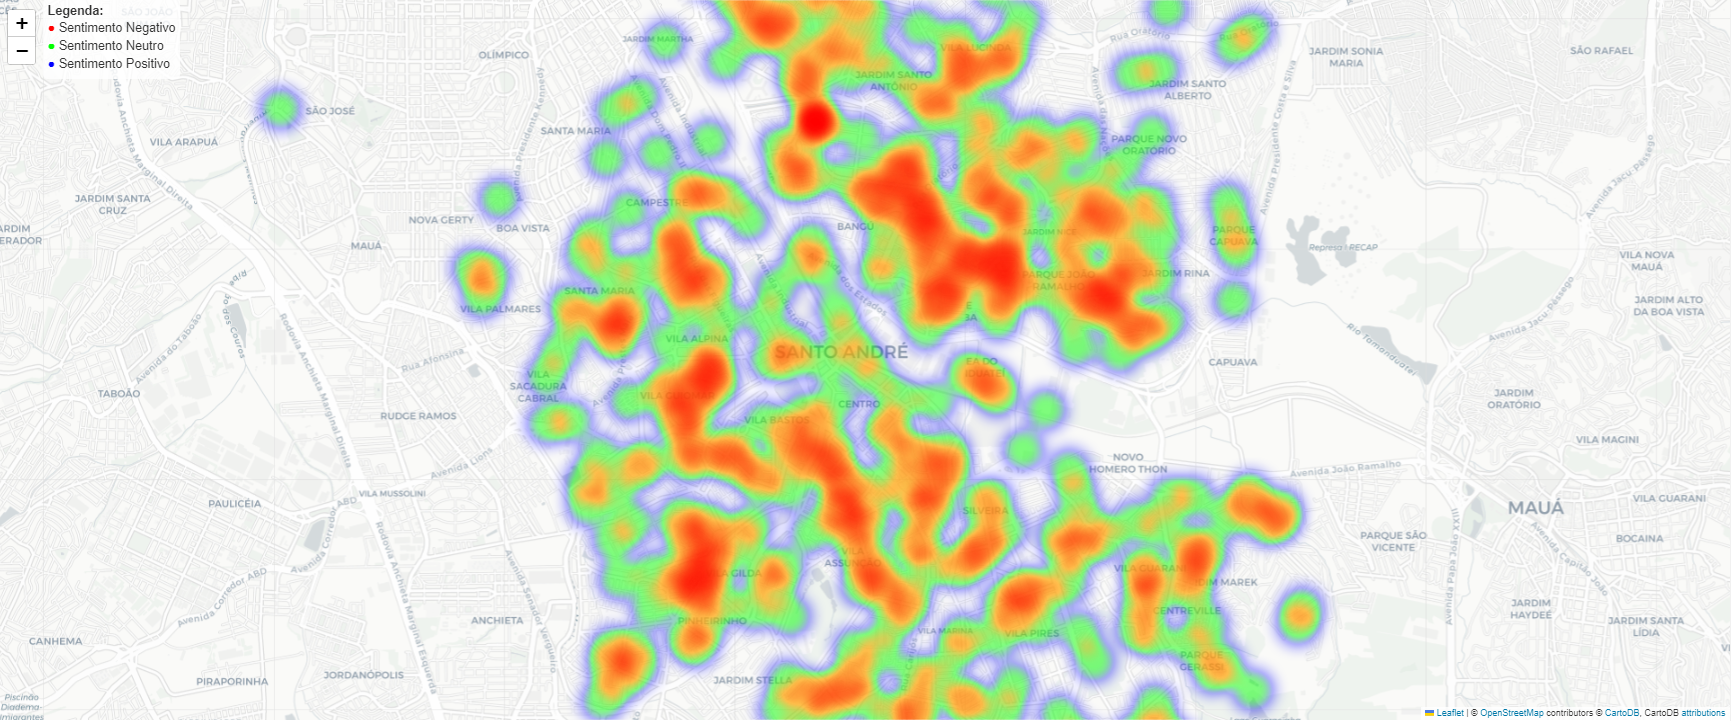
\includegraphics[width=0.7\textwidth]{images/heatmap_santo_andre.PNG}
	\caption{Heatmap de Pressão Social para Saúde Pública em Santo André}
	\label{fig:heatmap_santo_andre}
\end{figure}

Alguns eventos, como 'Coleta de container' e 'Limpeza de área pública', apresentam uma persona média predominantemente \textit{helper} e um score médio negativo. Isso sugere que esses eventos estão associados a preocupações legítimas da comunidade em relação à falta de serviços e manutenção adequados na cidade. A alta pontuação negativa no score médio indica um forte descontentamento em relação a esses problemas.

Por outro lado, eventos como 'Falta de água' têm uma persona média \textit{helper} e um score médio positivo, o que indica que a comunidade percebe esses eventos como situações em que a ajuda e a intervenção positiva são necessárias para resolver o problema da falta de água.

No entanto, também existem eventos com persona média \textit{complainer} e score médio negativo, como 'Infraestrura do Equipamento da Saúde' e 'Estabelecimento sem alvará'. Isso sugere que a comunidade está expressando críticas significativas em relação à infraestrutura de saúde e à conformidade com regulamentos, indicando uma insatisfação com essas áreas. A análise desses dados indica que a comunidade de Santo André tem uma visão polarizada sobre questões de saúde pública. Alguns eventos são percebidos como problemas sérios que exigem ação imediata, enquanto outros são vistos de maneira mais positiva, sugerindo um reconhecimento de oportunidades de melhoria. Essa diversidade de perspectivas destaca a complexidade da saúde pública como um tópico de pressão social.

\begin{figure}[htb]
	\centering
	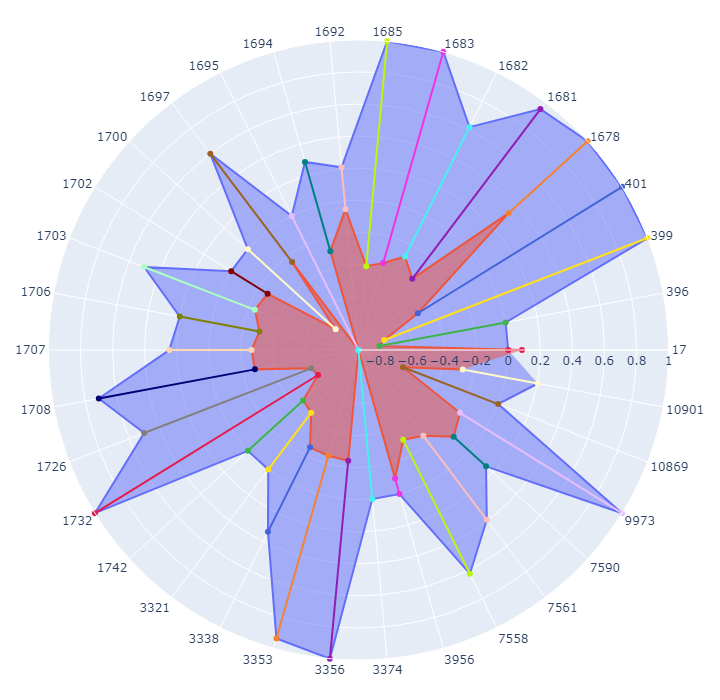
\includegraphics[width=0.7\textwidth]{images/social_barometer_santo_andre.png}
	\caption{social barometer santo andré}
	\label{fig:social_barometer_santo_andre}
\end{figure}

\begin{table}[htbp]
	\centering
	\caption{Pressão social do tópico Saúde Pública em Santo André}
	\label{tab:eventos_populares_sa}
	\begin{tabular}{|l|c|c|c|c|}
		\hline
		\textbf{Tipo de Evento}                               & \textbf{Eventos} & \textbf{Score} & \textbf{Persona} \\
		\hline
		3353:Aglomeração de pessoas                           & 13               & -0.2489        & 0.9375           \\
		\hline
		1707:Foco de mosquito da dengue/zika                  & 11               & -0.2663        & 0.2468           \\
		\hline
		1682:Estabelecimento com condição sanitária irregular & 10               & -0.2825        & 0.6190           \\
		\hline
		1694:Descarte irregular de lixo                       & 10               & -0.2928        & 0.2857           \\
		\hline
		1681:Ponto recorrente de poluição sonora              & 10               & -0.3996        & 0.9518           \\
		\hline
		1706:Infestação animais perigosos                     & 9                & -0.2904        & 0.2340           \\
		\hline
		10901:Esgoto a céu aberto                             & 9                & -0.2725        & 0.2037           \\
		\hline
		7590:Bueiro entupido                                  & 8                & -0.1304        & 0.1429           \\
		\hline
		7558:Ocupação irregular de área pública               & 8                & -0.3090        & 0.6364           \\
		\hline
		1683:Estabelecimento sem alvará                       & 6                & -0.3304        & 1.0000           \\
		\hline
		1685:Estabelecimento com acessibilidade irregular     & 6                & -0.4091        & 1.0000           \\
		\hline
		7561:Ponto de alagamento                              & 5                & -0.2627        & 0.3939           \\
		\hline
		1732:Área com risco de deslizamento                   & 5                & -0.4430        & 0.6667           \\
		\hline
		1697:Maus tratos a animais                            & 5                & -0.2470        & 0.6000           \\
		\hline
		3338:Iluminação pública irregular                     & 3                & -0.2093        & 0.2500           \\
		\hline
		1708:Ponto de tráfico de drogas                       & 3                & -0.2767        & 0.7143           \\
		\hline
		17:Rampa de acessibilidade irregular ou inexistente   & 3                & -0.2713        & 0.5000           \\
		\hline
		3356:Ônibus fora do horário/rota                      & 2                & -0.2401        & 1.0000           \\
		\hline
		3956:Faixa de pedestre apagada                        & 2                & -0.2330        & 0.0000           \\
		\hline
		1726:Patrimônio histórico em risco                    & 2                & -0.6174        & 0.5000           \\
		\hline
	\end{tabular}
\end{table}

No contexto da pandemia de COVID-19, os eventos mais populares ganham ainda mais relevância e urgência. 'Lixo' e 'Aglomeração de pessoas' emergem como líderes dessa lista, refletindo a forte ligação entre esses eventos e as preocupações essenciais relacionadas à saúde, higiene e segurança da comunidade, especialmente em tempos de crise sanitária. É notável que a categoria 'Aglomeração de pessoas' apresente uma persona média predominantemente \textit{helper}, sinalizando a disposição da comunidade para colaborar e se apoiar mutuamente na abordagem dessa preocupação crítica. No entanto, é importante observar que, apesar desse desejo de cooperação, esses eventos ainda mantêm um score médio elevado, o que evidencia a expressão de preocupações substanciais em relação à aglomeração, especialmente à luz das medidas de distanciamento social e precauções necessárias durante a pandemia.

\begin{figure}[htb]
	\centering
	\includegraphics[width=0.7\textwidth]{images/network_santo_andre_personas_map.png}
	\caption{Rede de eventos populares relacionados a Saúde Pública em Santo André}
	\label{fig:network_santo_andre_personas_map}
\end{figure}

Por outro lado, eventos relacionados a 'Lixo' têm uma persona média mais equilibrada entre \textit{helper} e \textit{complainer}, indicando uma mistura de percepções positivas e críticas. O score médio negativo nesses eventos reflete as preocupações da comunidade com o descarte irregular de lixo e a necessidade de melhorias na gestão de resíduos.

Em relação aos eventos mais populares, aqueles relacionados a 'Lixo' e 'Aglomeração de pessoas' lideram a lista. Esses eventos estão intimamente ligados às preocupações relacionadas à higiene, saúde e segurança da comunidade. A alta contagem de eventos nessas categorias reflete a importância dessas questões na mente dos cidadãos de Santo André. 'Aglomeração de pessoas' têm uma persona média predominantemente \textit{helper}, o que indica um desejo de colaboração e apoio mútuo para lidar com essa preocupação. No entanto, esses eventos também têm um score médio alto, sugerindo que a comunidade está expressando preocupações significativas em relação à aglomeração.

\begin{figure}[htb]
	\centering
	\includegraphics[width=0.7\textwidth]{images/wordcloud_santo_andre.png}
	\caption{Palavras mais frequentes nas postagens de Santo André}
	\label{fig:wordcloud_santo_andre}
\end{figure}

Em resumo, os dados refletem a complexidade da saúde pública em Santo André, com a comunidade demonstrando uma consciência aguçada das questões que afetam seu bem-estar. As reclamações estão concentradas em áreas críticas, e o diálogo positivo em alguns eventos indica um desejo de cooperação para resolver esses problemas. No entanto, a necessidade de ações eficazes por parte das autoridades e organizações responsáveis é evidente, considerando as preocupações legítimas da comunidade em relação à saúde pública na região.

\section{Trabalhos Futuros}

Em um contexto acadêmico, a abordagem central deste estudo reside na análise das câmaras de eco e na concepção do Colab como um barômetro social hiperlocal. Essa perspectiva oferece uma visão singular e abrangente das interações e percepções das comunidades locais em relação a tópicos polarizadores. No entanto, vale ressaltar que essa metodologia não se limita a seu emprego na pesquisa de câmaras de eco, sendo passível de extensão para diversas outras áreas de estudo.

A observação do Colab como um barômetro social hiperlocal implica em uma compreensão detalhada das opiniões, discussões e manifestações das comunidades locais em relação a questões específicas. Nesse contexto, a polarização emerge como um tema fundamental, visto que a plataforma proporciona uma visão inédita das dinâmicas de polarização no nível mais próximo da comunidade, indo além das análises tradicionais de polarização em escala mais ampla.

Essa abordagem também sugere que a pressão social hiperlocal proproem uma dimensão rica e relevante que pode ser investigada em outros contextos de pesquisa. Embora este estudo se concentre nas câmaras de eco e nas dinâmicas sociais específicas do Colab, é possível extrapolar essas heurísticas e metodologias para áreas de estudo diversas. Assim, abre-se a perspectiva para futuros trabalhos que explorem como a pressão social hiperlocal pode ser aplicada e analisada em campos como políticas públicas, meio ambiente, saúde pública, desenvolvimento urbano, engajamento cívico e conflitos sociais, entre outros.

Em pesquisas futuras, há um vasto campo a ser explorado no aprimoramento das heurísticas e métodos de análise da pressão social hiperlocal, especialmente no contexto de plataformas como o Colab. Uma das direções promissoras seria a incorporação de dimensões temporais e geolocalização de maneira mais robusta. Isso poderia ser alcançado através do desenvolvimento de algoritmos de análise de séries temporais para monitorar a evolução das discussões e do sentimento em torno de tópicos específicos ao longo do tempo. Compreender como as percepções e prioridades mudam sazonalmente ou em resposta a eventos específicos seria fundamental para uma análise mais holística. Além disso, a geolocalização desempenha um papel crítico na pressão social hiperlocal. A capacidade de mapear a localização precisa de eventos e discussões poderia permitir uma análise mais granular das dinâmicas das comunidades urbanas. Seria interessante explorar técnicas avançadas de geolocalização, como a análise de dados geoespaciais, para identificar padrões de pressão social em áreas urbanas específicas. Isso poderia ajudar as autoridades locais a direcionar recursos de forma mais eficaz e tomar decisões informadas sobre políticas públicas.

Também, vale a pena considerar a extensibilidade dessas heurísticas para outras redes sociais e plataformas além do Colab. A pressão social hiperlocal não é exclusiva de uma única plataforma, e compreender como ela se manifesta em diferentes contextos online poderia fornecer insights valiosos sobre o comportamento cívico e a participação pública em ambientes digitais variados. Isso abriria a porta para a criação de um framework mais amplo e aplicável a diversas situações. Outra área de pesquisa interessante seria a avaliação das implicações políticas e de governança da pressão social hiperlocal. Como as percepções locais podem influenciar as decisões políticas e a prestação de serviços públicos? Investigar como as vozes hiperlocais impactam as políticas urbanas e como as autoridades respondem a essas pressões seria um campo de estudo crítico para aprimorar a governança democrática.

A compreensão das dinâmicas da pressão social hiperlocal pode ser aplicada para informar a tomada de decisões políticas e a prestação de serviços públicos em nível local. Os governos municipais podem usar essa análise para identificar as principais preocupações dos cidadãos e a eficácia de suas políticas, adaptando-as de acordo com as demandas locais. Em estudos relacionados ao meio ambiente e desastres naturais, a pressão social hiperlocal pode ser usada para rastrear as preocupações e percepções das comunidades locais. Isso permite uma resposta mais eficaz a eventos climáticos extremos, poluição e outras questões ambientais. A análise da pressão social hiperlocal pode ser aplicada ao monitoramento de questões de saúde pública, como surtos de doenças infecciosas. A detecção rápida de preocupações da comunidade em relação à saúde pode ajudar as autoridades de saúde a tomar medidas preventivas e educativas. No contexto do desenvolvimento urbano, a pressão social hiperlocal pode ser usada para avaliar o impacto de projetos de infraestrutura, como construção de estradas, expansão de transporte público e desenvolvimento imobiliário. Isso permite uma análise mais detalhada das preocupações e necessidades das comunidades afetadas. Em estudos sobre conflitos e tensões sociais, a pressão social hiperlocal pode ser usada para identificar pontos de atrito em comunidades específicas. Isso pode ajudar na prevenção de conflitos e na promoção da coesão social.

Por fim, considerando a crescente importância da inteligência artificial e da análise de big data, explorar como essas tecnologias podem ser aplicadas de forma ética e eficaz na detecção e análise da pressão social hiperlocal é uma área promissora de pesquisa. O desenvolvimento de ferramentas automatizadas para identificar tópicos de pressão e monitorar o sentimento em tempo real poderia revolucionar a forma como as cidades respondem às demandas de seus cidadãos. Há uma série de oportunidades empolgantes para aprimorar nossas abordagens de análise da pressão social hiperlocal, incorporando dimensões temporais, geolocalização e estendendo essas heurísticas para diferentes plataformas e contextos. Isso não apenas enriqueceria nosso entendimento das comunidades urbanas, mas também teria implicações práticas significativas para a governança local e o envolvimento cívico.

\section{Conclusões}

No decorrer deste capítulo, exploramos as dinâmicas da opinião pública no Colab, uma plataforma que abriga discussões sobre tópicos urbanos diversos. Nossas análises revelaram uma diversidade de perspectivas e abordagens por parte dos usuários em relação a questões urbanas. Observamos que não há uma única persona predominante, variando amplamente entre eventos, refletindo a complexidade das questões urbanas. Isso indica que a comunidade do Colab lida com diferentes problemas de maneiras variadas, desde a busca por soluções até a expressão de críticas construtivas ou negativas.

Surpreendentemente, mesmo nas discussões em que predominam personas \textit{helper}, ainda podem surgir críticas construtivas, e vice-versa. Isso demonstra a disposição dos usuários em considerar diferentes perspectivas e contribuir para melhorias, independentemente de sua atitude inicial em relação ao problema. Além disso, apesar de algumas polarizações em debates políticos e tópicos sensíveis, a maioria dos usuários parece comprometida em abordar e resolver os desafios urbanos. A presença de personas \textit{helper} indica uma disposição para encontrar soluções construtivas, mesmo em meio a divergências.

A aplicação de abordagens de engenharia de software foi essencial para nossa análise, permitindo-nos desenvolver heurísticas para medir a opinião média e as personas dos usuários em relação a diferentes eventos urbanos. Essas heurísticas serviram de base para representações visuais, como o gráfico de radar, que auxiliaram na visualização das dinâmicas sociais de forma acessível. Além disso, a coleta de dados estruturados por meio de um modelo bem definido foi fundamental para organizar as informações e facilitar a análise. Integrando a tecnologia de aprendizado de máquina na forma de algoritmos de classificação e processamento de linguagem natural, automatizamos a análise de texto, economizando tempo e recursos. Isso nos permitiu examinar um grande volume de dados em larga escala.

Aqui reside uma conexão profunda entre a fenomenologia e a engenharia de software. Assim como a fenomenologia busca compreender as experiências subjetivas de indivíduos, nossa abordagem de engenharia de software nos permitiu mergulhar profundamente nas experiências dos usuários do Colab, revelando as nuances de suas interações e perspectivas. Ao aplicar heurísticas para medir opiniões e personas, criamos uma lente através da qual podemos observar as complexidades das redes sociais em escala.

Além disso, reconhecemos a importância de integrar os resultados de nossa análise com os tomadores de decisão, como agências governamentais e organizações da sociedade civil. Isso garante que nossas descobertas sejam utilizadas para informar políticas e ações práticas, promovendo uma governança mais informada e eficaz.

A análise também nos levou a explorar o fenômeno da polarização, que é amplamente observado em ambientes digitais, como redes sociais. Identificamos como as plataformas digitais podem contribuir para a formação de câmaras de eco e bolhas de filtro, reforçando crenças preexistentes e restringindo a exposição a diferentes perspectivas. No entanto, também reconhecemos que o ciberespaço, como definido por Levy, é um ambiente multifacetado, onde diversas vozes e visões coexistem.

Levy nos lembra que a cibercultura é caracterizada pela diversidade de atores, projetos e interpretações, frequentemente em oposição. O ciberespaço, apesar de desafios, oferece oportunidades para o diálogo e a colaboração entre diferentes perspectivas culturais. Isso é particularmente relevante no contexto do Colab, onde a diversidade de perspectivas é uma força que permite a consideração de uma ampla gama de soluções para os problemas urbanos.

Ao incorporar a análise de sentimentos e personas dos usuários em nossa compreensão do Colab, estamos agregando uma dimensão adicional à nossa capacidade de medir a pressão social hiperlocal. Isso nos permite identificar áreas de polarização e tensão dentro da comunidade, bem como oportunidades para promover o diálogo e a colaboração. A abordagem de Levy à cibercultura destaca a interconexão e a valorização da diversidade de perspectivas, e o Colab tem o potencial de se tornar um espaço inclusivo para o diálogo cidadão e a construção de comunidades informadas e coesas.

Em última análise, o Colab, como um 'barômetro social hiperlocal' e uma plataforma de cidadania, tem o potencial de desempenhar um papel crucial na promoção da participação cidadã, no engajamento construtivo e na melhoria das condições urbanas. À medida que continuamos a valorizar a diversidade de perspectivas e a buscar soluções colaborativas, podemos avançar na construção de cidades mais eficientes, seguras e inclusivas, em um ciberespaço que amplifica tanto os desafios quanto as oportunidades da opinião pública. Este capítulo nos conduziu à compreensão de que o Colab é um espaço de convergência, onde perspectivas culturais variadas têm a oportunidade de dialogar e colaborar. A diversidade de vozes é a essência da cibercultura, e o Colab é um exemplo poderoso disso.

No próximo capítulo, continuaremos a explorar a complexidade das redes sociais, mas com um foco específico na detecção de câmaras de eco. Essa pesquisa se conecta diretamente ao nosso experimento atual, onde desenvolvemos heurísticas para medir a opinião média e as personas dos usuários em relação a diferentes tipos de eventos. As heurísticas e os insights obtidos até agora servirão como base fundamental para a próxima etapa de nossa investigação.

Além disso, nosso conjunto de dados abrange não apenas os eventos criados pelos usuários, classificados por score e persona, mas também inclui informações detalhadas sobre os relacionamentos de rede social entre os usuários das três cidades, revelando os usuários mais influentes, cada seguidor e quantos usuários cada pessoa segue além dos tipos de eventos com os quais interagem. Cada evento também é enriquecido com comentários e likes, proporcionando uma visão mais completa das interações dos usuários. Com base nesses dados e nas heurísticas criadas a partir deles, seremos capazes de inferir não apenas a opinião média dos usuários em relação a diversos tipos de evento, mas também avaliar a homogeneidade de opiniões com base no tipo de evento com o qual cada usuário interage com mais frequência e compará-lo com o tipo de evento mais interagido pelos membros de sua rede social. Com cada evento, comentário ou interação, os usuários não apenas expressam uma opinião, mas também se engajam em um processo de co-criação e interpretação de significado no ciberespaço. Portanto, as ideias de barômetro social hiperlocal, pressão social e detecção de câmaras de eco estão intrinsecamente conectadas porque elas refletem as dinâmicas e nuances das relações humanas que se desdobram no ciberespaço. O conceito de 'barômetro social hiperlocal' captura a essência de como as interações individuais se somam para criar um panorama mais amplo da opinião pública em uma região específica. Ao mesmo tempo, a pressão social revela como os usuários influentes podem moldar ou direcionar as opiniões e interações dentro de suas redes. Finalmente, a detecção de câmaras de eco é uma consequência direta dessas interações, mostrando como grupos de usuários podem se tornar insulares em suas opiniões, reforçando crenças e perspectivas semelhantes.

Dentro dessa complexa teia de relacionamentos e interações, um usuário não é apenas um ponto de dados, mas uma entidade viva que busca conexão, expressão e entendimento. Os dados que coletamos e as heurísticas que aplicamos, portanto, não são meros exercícios técnicos, contudo, é fundamental lembrar que por trás desses dados, existem indivíduos com experiências reais e tangíveis. O pensamento de Heidegger sobre a 'técnificação das mãos' sugere uma preocupação com a maneira pela qual a tecnologia pode distanciar o ser humano de uma vivência autêntica do mundo. Quando um usuário do Colab cria um evento ou interage na plataforma, essa 'técnificação' pode estar presente, influenciando como ele percebe e se relaciona com o espaço digital. Nesse sentido, a própria criação de heurísticas e o uso da engenharia de software podem ser vistos como uma extensão desse processo de 'técnificação'. Por outro lado, Merleau-Ponty, com sua ênfase na corporeidade e percepção, serve como um lembrete de que as interações no Colab são manifestações de experiências corpóreas e perceptivas dos usuários.

A polarização, as câmaras de eco e até mesmo as análises de sentimentos não são meros produtos técnicos, mas emergem das experiências vividas e sentidas das pessoas. Ao avançarmos na integração entre engenharia de software e fenomenologia, é crucial lembrar que cada clique, postagem ou interação no Colab tem sua origem na experiência humana. Deste modo, nossas análises, embora apoiadas por ferramentas tecnológicas sofisticadas, devem sempre manter a centralidade do ser humano e suas experiências. Assim, mesmo quando exploramos as complexidades técnicas e analíticas, reconhecemos que elas servem para nos aproximar, e não distanciar, das nuances e riquezas da experiência humana no ciberespaço e na vida real.